\documentclass[11pt, a4paper]{article} %tamaño mínimo de letra 11pto.

\usepackage{graphicx} 
%\usepackage[english]{babel} %Español 
\usepackage[utf8]{inputenc} %Para poder poner tildes
\usepackage{vmargin} %Para modificar los márgenes
\setmargins{2.5cm}{1.5cm}{16.5cm}{23.42cm}{10pt}{1cm}{0pt}{2cm}
%margen izquierdo, superior, anchura del texto, altura del texto, altura de los encabezados, 
% entre el texto y los encabezados, altura del pie de página, espacio entre el texto y el pie de página

% introducido por mi 
\usepackage{amsmath,amsfonts,amssymb} % ecuaciones
\usepackage{siunitx}
\usepackage{fancyhdr} % headers y footers
\usepackage{esint} % integrales cerradas
\usepackage{bbold} % para meter matriz identidad
\usepackage{graphicx} % estos dos para una figura
\usepackage{caption}
\usepackage{subcaption}
\usepackage{pdfpages} % para incluir declaracion IA
\usepackage{float}
\usepackage[toc,page]{appendix}
%\usepackage{physics}
\usepackage{bm}
%\usepackage[numbers,sort&compress]{natbib} % for bibliography
\usepackage[inkscape=false]{svg} % add svg files
\usepackage{hyperref} % to add video
\usepackage{tikz} % to generate plots 
\usepackage{setspace} % to space out text lines
\usepackage[T1]{fontenc}
\usepackage{calc}
\usepackage{wrapfig}
\usetikzlibrary{decorations.markings,arrows.meta}
\usetikzlibrary{calc}
\usepackage{xcolor}
\definecolor{titlecolor}{HTML}{4884d6}
\usepackage{pgfplots}
\pgfplotsset{compat=1.18}
\usepgfplotslibrary{groupplots}
%\usepackage{standalone}
\newcolumntype{C}{>{$}c<{$}}

\usepackage[style=numeric,sorting=none, backend=biber]{biblatex}  % Load biblatex with the 'verbose' style for full citations in footnotes
\addbibresource{bibliography.bib}

\setlength{\parskip}{\baselineskip}
\renewcommand{\baselinestretch}{1.2}

\newcommand{\xv}{\vec{x}}
\newcommand{\yv}{\vec{y}}
\newcommand{\xd}{\dot{x}}
\newcommand{\xdd}{\ddot{x}}
\newcommand{\yd}{\dot{y}}
\newcommand{\ydd}{\ddot{y}}
\newcommand{\bigO}{\mathcal{O}}
\newcommand{\Th}{\theta}
\newcommand{\zd}{\dot{z}}
\newcommand{\w}{\omega}

\newcommand{\yinyanglobe}[3]{
    \begin{scope}[rotate=#1]
        \fill[#2] (0,0) 
            arc[start angle=-90, end angle=90, radius=0.5cm] 
            arc[start angle=90, end angle=-90, radius=1cm]
            arc[start angle=90, end angle=270, radius=0.5cm] -- cycle;
            
        \fill[#3] (0, 1) circle (0.25cm);
    \end{scope}
}
\tikzset{
    >={Stealth[length=3pt]}, % Standard, clean arrowhead
    % Custom style to place a single arrow at the halfway point of a path
    cleanflow/.style={
        decoration={
            markings,
            mark=at position 0.5 with {\arrow{>}}
        },
        postaction={decorate}
    },
    stable/.style={line width=1.5pt, draw=black},
    thinarc/.style={line width=0.7pt, draw=black!90},
    textlabel/.style={font=\small\selectfont, text=black}
}

\tikzset{
  flow/.style={
    decoration={
      markings,
      mark=at position #1 with {\arrow[scale=1.3]{stealth}}
    },
    postaction={decorate}
  },
  flow/.default=0.55
}

\begin{document}

\begin{titlepage}
  \centering

  %% Top rule
  {\color{titlecolor}\rule{\linewidth}{0.6mm}}\\[0.5cm]

  %% Title
  {\Huge\bfseries Spin-mometum locking in a mechanical altermagnet of non-reciprocal actuators \par}
  \vspace{0.3cm}
  %{\large Explanatory subtitle \par}

  %% Bottom rule under title
  \vspace{0.3cm}
  {\color{titlecolor}\rule{\linewidth}{0.6mm}}\\[1.5cm]

  %% Degree info
  {\large Master's Thesis \par}
  \vspace{0.3cm}
  {\large  \par}
  %\vspace{0.3cm}
  \begin{figure}
    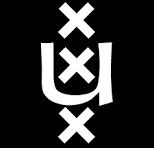
\includegraphics[height=2cm]{Uva_logo.png}
    \hfill
    
\includegraphics[height=2cm]{vu_logo.png}
  \end{figure}
  {\large University of Amsterdam \\ Vrije Universiteit Amsterdam \par}

  \vfill

  %% Info table
  \begin{tabular}{@{} l l @{}}
    \textbf{Author:}             & Victor Garcia      \\
    \textbf{Student number:}     & 15721949                \\[0.5em]
    \textbf{First supervisor:}   & Corentin Coulais            \\
    \textbf{Second supervisor:}  & Jasper van Wezel           \\
    %\textbf{Company supervisor:} & Company Supervisor        \\[0.5em]
    \textbf{Period:}             & 2025-2026  \\
    %\textbf{Hand-in date:}       &            \\
    %\textbf{Study points:}       & XX ECTS                   \\
  \end{tabular}

  \vfill

  %% Bottom rule
  {\color{titlecolor}\rule{\linewidth}{0.6mm}}

\end{titlepage}

\section*{Abstract}

Altermagnets are a recently discovered ordered magnetic phase with novel properties promising in spintronics. 
They are characterized by the rotation relationship between spin sublattices. 
We study the properties of such system in a classical setting. 
We build a mechanical apparatus composed of actuators which can be arranged in a variety of geometries, leading to different symmetries. 
The magnetic spin is replaced by the chirality of oscillators, using non-reciprocal interactions between pairs of actuators. 
We observe synchronization of actuators and selective propagation in 1D systems. 
In the altermagnet 2D lattice, we find spin/chirality-momentum locking and a frustrated bistable system.
The experimental results are corroborated by theoretical models and simulations. 

\newpage
\tableofcontents
\newpage

\section{Introduction}
\label{sec:intro}
% Describe concepts like in presentations: wave guidance, altermagnets, non-Hermitian physics.

% First, let me say one-line summary punchline of the project, and then we can untangle the meaning of the words. 

The main purpose of this thesis is to study wave guidance in a mechanical realization of an altermagnet. 
%Let's start with wave guidance. 
Wave guidance is the ability to direct waves along a certain path, often with minimal loss or distortion. 
It is crucial in various applications, from telecommunications to medical imaging. 
We build a mechanical metamaterial made up of springs and actuators, with the symmetry of an altermagnet. 
The metamaterial reproduces some properties from the original magnetic phase, with chiral phonons instead of 
spin up and down electrons. 
%The most important feature is what wave, or particle excitation, one employs. 
% Here, we are using 
% quantum mechanical language to say that particles are the energy excitations of fields, and these fields behave like waves.
% One could use electrons, photons, phonons, magnons, etc to propagate information from one point to another.


\subsection{Altermagnets}
\label{subsec:altermagnets}

\begin{figure}[hbtp]
    \begin{center}
        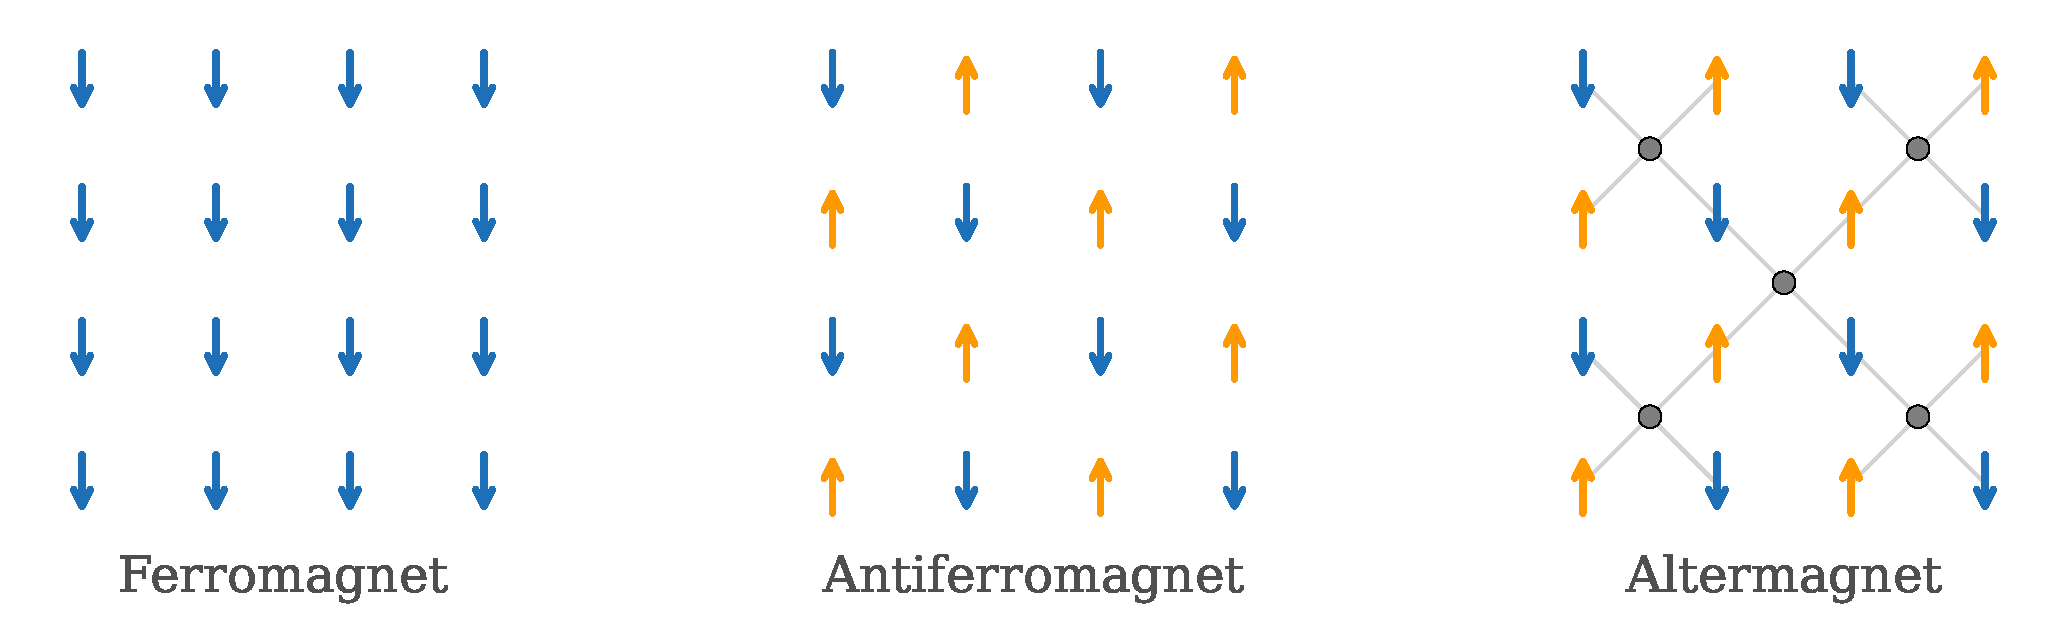
\includegraphics[width=0.8\textwidth]{magnetic_phases.pdf}
        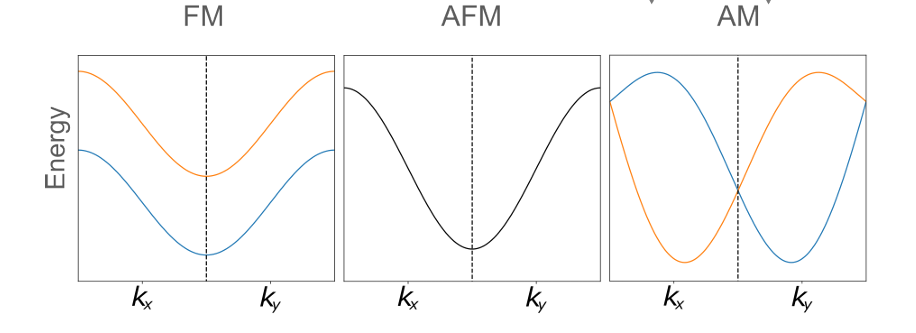
\includegraphics[width=\textwidth]{bands_altermagnet.png}
        \caption{\textbf{Collinearly-ordered magnetic phases: ferromagnets, antiferromagnets and altermagnets.}
            \textbf{Top:} diagram of the lattice spins in ferromagnet, antiferromagnet and altermagnet, from left to right.
        \textbf{Bottom:} schematic representation of their band structure. The focus is on the relationship between the spin-up band in 
        orange with the spin-down band in blue.}
        \label{fig:magnetism}
    \end{center}
\end{figure}

Before introducing altermagnets, we must briefly mention ordinary collinearly ordered magnetism. In traditional magnets, 
the magnetic moments of atoms, or spins for short, align in a uniform direction, leading to a net magnetic field. These materials are called ferromagnets. 
We can also find in nature materials whose spins tend to point in opposite directions to their neighbours, cancelling the net magnetic field. 
These materials are called antiferromagnets. However, most materials do not exhibit 
any magnetic order at all. We focus on paramagnets, which are characterized by a field of randomly oriented spins. 
The way we classify theoretically different materials in any of these three categories is using symmetries. As we often do, we start 
with the most symmetric of the three: paramagnets. In these materials, the spins are randomly oriented. 
The average properties, the expectation values, of the magnetic system are invariant under spin-rotations, 
which are transformations that only rotate the spin degrees of freedom. As a consequence, paramagnets are also invariant under 
time reversal, meaning that if we reverse the direction of time, the system looks the same. But what does reversing time mean? It simply means that 
if we were to film the system with a camera and then play the footage backwards, we wouldn't be able to tell the difference. At the level of equations, 
what we do is add a minus sign to time. This has an effect on some of the physical quantities. For instance, the sign of the linear momentum changes, 
because we are playing the movie backwards. The same happens to angular momentum, and more specifically, 
to spin angular momentum, which also changes sign under time reversal. Time reversal flips a spin up into spin down and vice versa, so it 
is a particular case of a spin-rotation transformation.
Since paramagnets have randomly oriented spins, flipping the spins leaves the system invariant. We say paramagnets are time reversal symmetric.
Do antiferromagnets and magnets also have these symmetries? The key is that they do not. 
Ferromagnets and antiferromagnets break spin-rotation symmetry because the spins align and disalign in a specific direction. Thus, they also 
break time reversal symmetry. Nevertheless, one can combine spin transformations, acting only on spins, with real space transformations, 
acting only on the lattice, and obtain symmetries. We consider these two types of transformations to be uncoupled from each other.
For antiferromagnets, the combination of time reversal with translation is a symmetry (also with inversion). 
This happens because translations swap the two opposite spin sublattices. 
This symmetry along with electrons having half-integer spin 
(which makes the antiunitary symmetry operator square to -1), leads to Kramer's theorem.  
The theorem states that every energy level is at least doubly degenerate. 
In plain language, one can have two electrons, one with spin up 
and one with spin down, occupying the same energy level, leading to spin degenerate bands. Ferromagnets do not possess this symmetry. 
Kramer's degeneracy does not hold for them, and they have spin-dependent bands. Spin up and down electrons have different 
energy band structure and thus they behave differently. 
So the way we can tell apart different magnetic orders, or phases in general, 
is by looking at which symmetries they have and which symmetries they break.
%A small note is that antiferromagnets do preserve a combination of time reversal and a spatial translation that swaps the two opposite spin sublattices. 
%Time reversal symmetry,  degeneracy in antiferromagnets.  
Now we can tackle altermagnets. Altermagnets were recently discovered because they had strange properties, like anomalous qunatum Hall effect. 
They share some properties with ferromagnets and some 
other with antiferromagnets. At first they were called anomalous antiferromagnets, but then 
Smejkal \cite{smejkal2022} realised they had a different symmetry, 
so it was a new phase of matter. Altermagnets are another collinearly ordered magnetic phase, but with different symmetries.
Like antiferromagnets, they are made up of two spin sublattices, up and down.
They break the antiferromagnet symmetry, i.e. the combination of time reversal and translation. However, they are
symmetric under the combination of time reversal and a real space rotation. 
This allows them to have spin-split bands, like ferromagnets. However, altermagnets have no net magnetic field, like antiferromagnets.  

\begin{figure}[hbtp]
\centering
  \begin{subfigure}[b]{0.38\textwidth}
    \begin{center}
       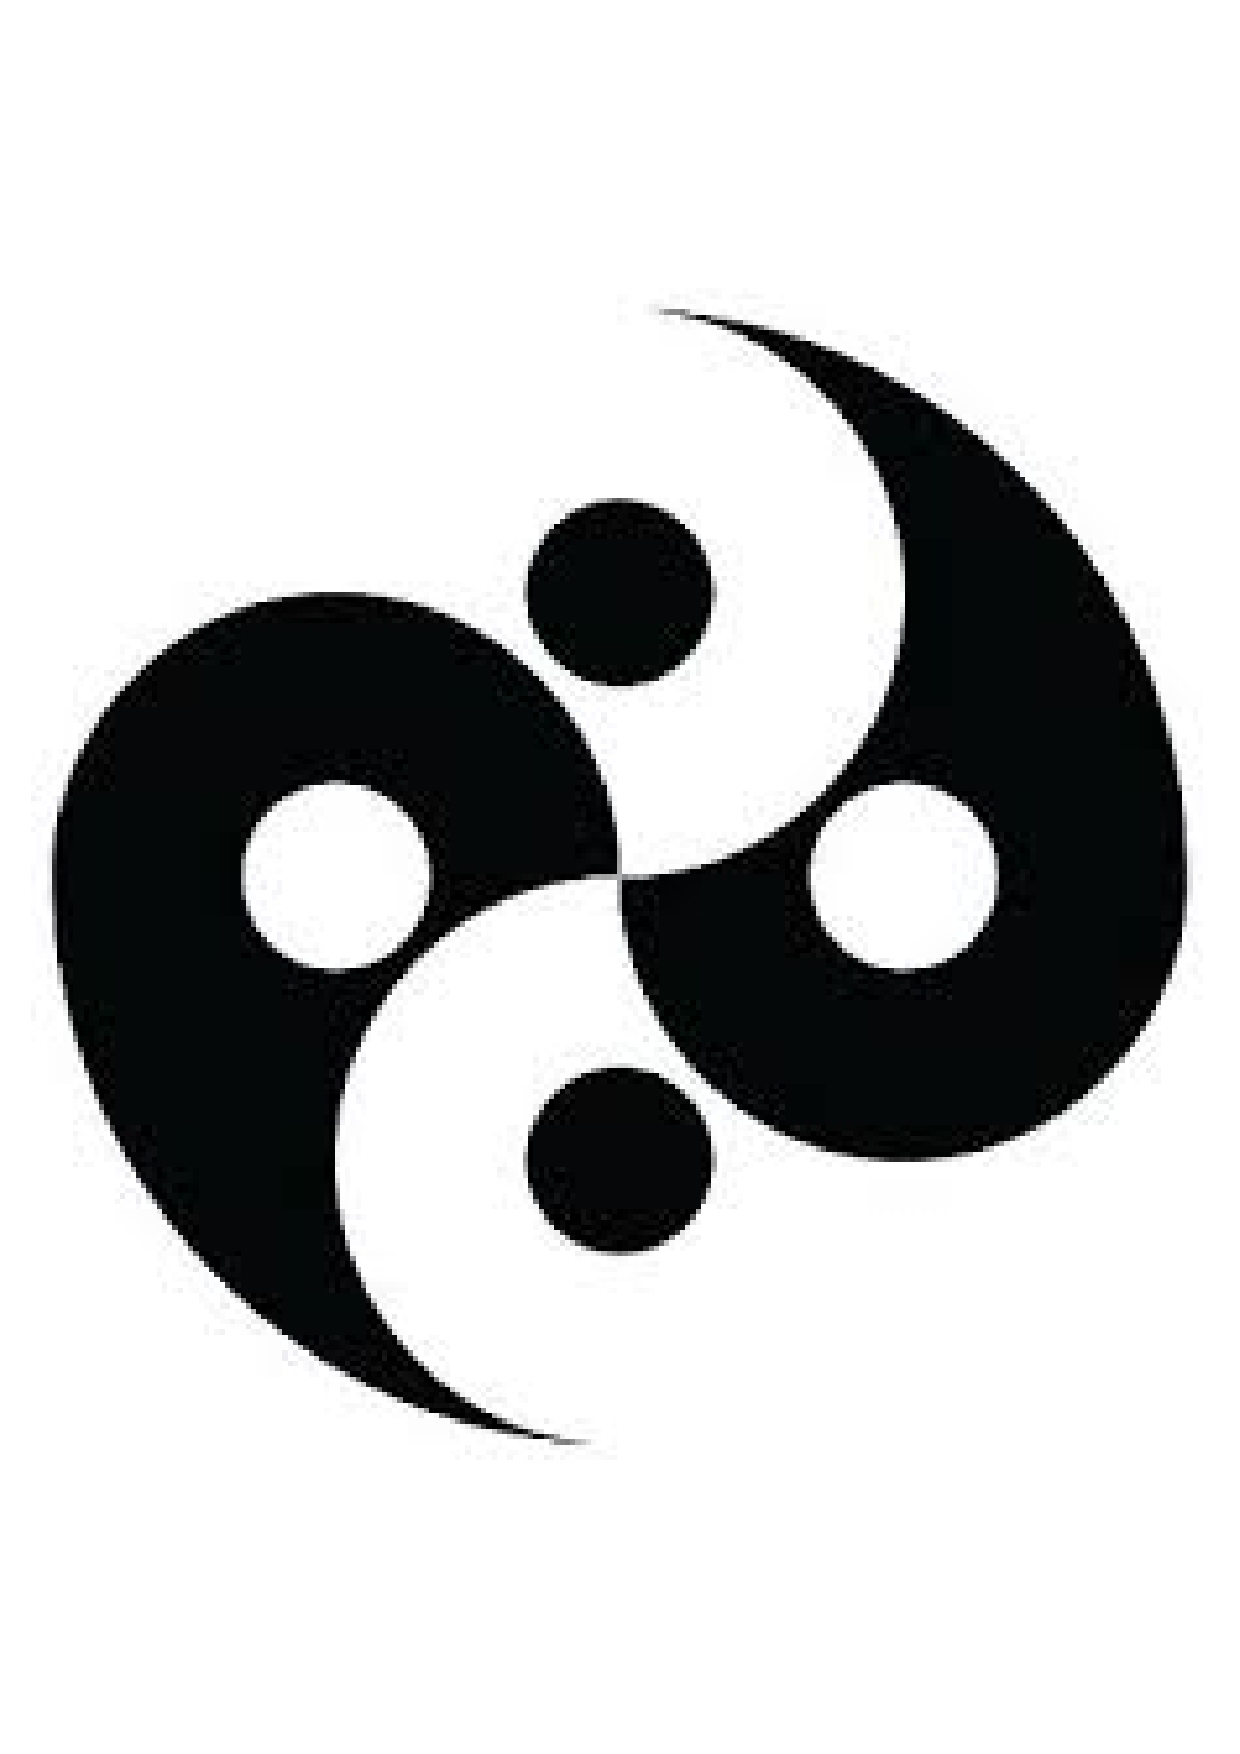
\includegraphics[scale=0.2]{yingyang.pdf} 
       \caption{}
       \label{fig:yinyang}
    \end{center}
  \end{subfigure}
  \begin{subfigure}[b]{0.58\textwidth}
    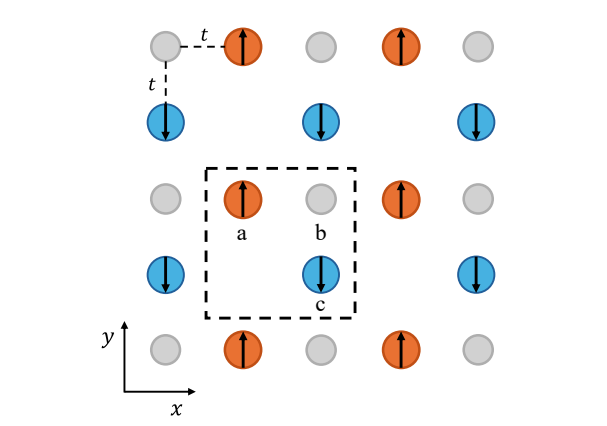
\includegraphics[width = \textwidth]{Lieb_lattice.png}
    \caption{}
    \label{fig:Lieb}
  \end{subfigure}
        \caption{\textbf{Systems with $C_4\mathcal{T}$ symmetry.}
            \textbf{\ref{fig:yinyang}} Yin-yang symbol with four lobes. 
            \textbf{\ref{fig:Lieb}} Altermagnetic Lieb lattice \cite{visser2026}. 
        They both share the spin/colour flip combined with 90º rotation symmetry.}
        \label{Lieb_lattice}
    \end{figure} 

We focus on a particular model of altermagnet called the Lieb lattice \cite{Lieb}. The particular symmetry of this model 
is time reversal combined with a 90º lattice rotation. We denote it as $C_4\mathcal{T}$. 
As shown in figure \ref{Lieb_lattice}, it is a two-dimensional square lattice 
with a three-atom motif: one spin up atom, one spin down atom, and one neutral atom. The neutral atom is not magnetic, 
and thus has no spin degree of freedom. 
On figure \ref{Lieb_lattice}, one can notice 
that the nearest neighbours of any spin up site are non-magnetic sites at each side, in the horizontal direction. 
On the contrary, for spin down sites, the nearest neighbours are non-magnetic sites in the vertical direction.
The spin atoms create a magnetic field, which has an effect on the electron spin. The field breaks the $\mathrm{SU}(2)$ 
spin symmetry of electrons down to $\mathcal{Z}_2$. This means that the electron collapses to either spin up or spin down.
The energy is minimized when the spin of the electron and atom are aligned.
If we only allow hopping between nearest neighbours, we can intuitively predict that spin up electrons are 
more likely to move in the horizontal direction, while spin down electrons prefer the vertical direction. 
This means electrons with different spin propagate in different directions. We call this effect spin-momentum locking 
\cite{kane_TI}. The reason why it happens is the symmetry of the altermagnet. 

One can generalize the altermagnet symmetry $C_4T$ to other systems by replacing the spin degree of freedom with other two-level variables.
This opens the door to realizing altermagnet-like behaviour in various physical platforms. 
For example, \cite{kim2025photonicaltermagnets} have replaced spin with the photon's polarization states, 
and they designed photonic crystals that exhibit altermagnet-like properties.
Similarly, \cite{visser2026} used electric dipoles to build an alterelectric. 
The focus of this thesis is to explore spin-momentum locking in a mechanical Lieb lattice, 
where the two-level variable is chirality of the oscillator. Spin up and down are replaced by clockwise and counterclockwise motion. 
We achieve it using non-reciprocity.
%to other rotational symmetries combined with time-reversal, like $C_6T$.

\subsection{Non-reciprocity}
\label{subsec:non-reciprocity}

\begin{figure}[htbp]
\centering
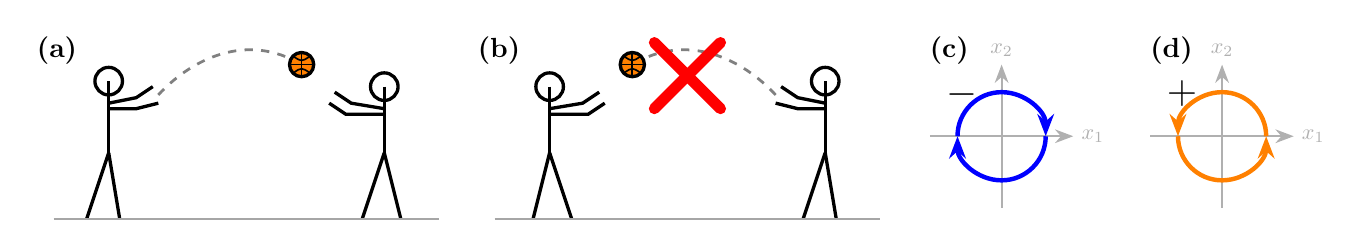
\begin{tikzpicture}[>=Stealth, line width=1.2pt, scale=0.7]

    % Color definition
    \definecolor{dimmed}{HTML}{B0B0B0} % Soft Grey

    % =========================================================================
    % SUBFIGURE A: Left to Right Pass (Success)
    % =========================================================================
    \begin{scope}[shift={(0,0)}]
        % --- Left Person (Passer) ---
        \coordinate (L-head) at (0, 2.5);
        \coordinate (L-pelvis) at (0, 1.2);
        \draw[fill=white] (L-head) circle (0.25);
        \draw (L-head) -- (L-pelvis);
        \draw (L-pelvis) -- (-0.4, 0);
        \draw (L-pelvis) -- (0.2, 0);
        \draw (0, 2.1) -- (0.5, 2.2) -- (0.8, 2.4);
        \draw (0, 2.0) -- (0.5, 2.0) -- (0.9, 2.1);

        % --- Right Person (Receiver) ---
        \coordinate (R-head) at (5, 2.4);
        \coordinate (R-pelvis) at (5, 1.2);
        \draw[fill=white] (R-head) circle (0.25);
        \draw (R-head) -- (R-pelvis);
        \draw (R-pelvis) -- (4.6, 0);
        \draw (R-pelvis) -- (5.3, 0);
        \draw (5, 2.0) -- (4.4, 2.1) -- (4.1, 2.3);
        \draw (5, 1.9) -- (4.3, 1.9) -- (4.0, 2.1);

        % --- Trajectory & Ball ---
        \coordinate (StartBall) at (0.9, 2.25);
        \coordinate (CurrentBall) at (3.5, 2.8);
        \draw[dashed, gray, line width=1pt] (StartBall) .. controls (1.5, 2.9) and (2.5, 3.4) .. (CurrentBall);

        \draw[fill=orange, draw=black] (CurrentBall) circle (0.22);
        \draw[line width=0.6pt] (3.5, 3.02) -- (3.5, 2.58); 
        \draw[line width=0.6pt] (3.28, 2.8) -- (3.72, 2.8); 
        \draw[line width=0.6pt] (3.35, 2.95) .. controls (3.5, 2.85) .. (3.65, 2.95); 
        \draw[line width=0.6pt] (3.35, 2.65) .. controls (3.5, 2.75) .. (3.65, 2.65); 

        % --- Ground Line ---
        \draw[line width=0.8pt, gray!70] (-1, 0) -- (6, 0);
        % --- Inside Scope A (Success Pass) ---
        \node[font=\bfseries, anchor=north west] at (-1.5, 3.5) {(a)};
    \end{scope}

    % =========================================================================
    % SUBFIGURE B: Right to Left Pass (Blocked/No Pass)
    % =========================================================================
    \begin{scope}[shift={(8,0)}]
        % --- Left Person (Receiver) ---
        \coordinate (L2-head) at (0, 2.4);
        \coordinate (L2-pelvis) at (0, 1.2);
        \draw[fill=white] (L2-head) circle (0.25);
        \draw (L2-head) -- (L2-pelvis);
        \draw (L2-pelvis) -- (-0.3, 0);
        \draw (L2-pelvis) -- (0.4, 0);
        \draw (0, 2.0) -- (0.6, 2.1) -- (0.9, 2.3);
        \draw (0, 1.9) -- (0.7, 1.9) -- (1.0, 2.1);

        % --- Right Person (Passer) ---
        \coordinate (R2-head) at (5, 2.5);
        \coordinate (R2-pelvis) at (5, 1.2);
        \draw[fill=white] (R2-head) circle (0.25);
        \draw (R2-head) -- (R2-pelvis);
        \draw (R2-pelvis) -- (4.6, 0);
        \draw (R2-pelvis) -- (5.2, 0);
        \draw (5, 2.1) -- (4.5, 2.2) -- (4.2, 2.4);
        \draw (5, 2.0) -- (4.5, 2.0) -- (4.1, 2.1);

        % --- Trajectory & Ball ---
        \coordinate (StartBall2) at (4.1, 2.25);
        \coordinate (CurrentBall2) at (1.5, 2.8);
        \draw[dashed, gray, line width=1pt] (StartBall2) .. controls (3.5, 2.9) and (2.5, 3.4) .. (CurrentBall2);

        \draw[fill=orange, draw=black] (CurrentBall2) circle (0.22);
        \draw[line width=0.6pt] (1.5, 3.02) -- (1.5, 2.58); 
        \draw[line width=0.6pt] (1.28, 2.8) -- (1.72, 2.8); 
        \draw[line width=0.6pt] (1.35, 2.95) .. controls (1.5, 2.85) .. (1.65, 2.95); 
        \draw[line width=0.6pt] (1.35, 2.65) .. controls (1.5, 2.75) .. (1.65, 2.65); 

        % --- Ground Line ---
        \draw[line width=0.8pt, gray!70] (-1, 0) -- (6, 0);

        % --- BIG RED BLOCKING CROSS ---
        \coordinate (CrossCenter) at (2.5, 2.6);
        \draw[line width=4pt, red, cap=round] ($(CrossCenter)+(-0.6,-0.6)$) -- ($(CrossCenter)+(0.6,0.6)$);
        \draw[line width=4pt, red, cap=round] ($(CrossCenter)+(-0.6,0.6)$) -- ($(CrossCenter)+(0.6,-0.6)$);
        % --- Inside Scope B (Blocked Pass) ---
        \node[font=\bfseries, anchor=north west] at (-1.5, 3.5) {(b)};
    \end{scope}

    % =========================================================================
    % SUBPLOT C: Clockwise (-)
    % =========================================================================
    \begin{scope}[shift={(16.2, 1.5)}]
        % Dimmed Axes (x_1 and x_2)
        \draw[->, dimmed, thick] (-1.3,0) -- (1.3,0) node[right, scale=0.8] {$x_1$};
        \draw[->, dimmed, thick] (0,-1.3) -- (0,1.3) node[above, scale=0.8] {$x_2$};
        
        % Clockwise Circle
        \draw[-{Stealth[length=8pt, width=6pt]}, ultra thick, blue] (-0.8,0) arc (180:0:0.8);
        \draw[-{Stealth[length=8pt, width=6pt]}, ultra thick, blue] (0.8,0) arc (0:-180:0.8);
        
        % Sign in Top Left
        \node[font=\Large\bfseries, anchor=north west] at (-1.2, 1.2) {$-$};
        % --- Inside Scope C (Clockwise) ---
        \node[font=\bfseries, anchor=north west] at (-1.5, 2.0) {(c)};
    \end{scope}

    % =========================================================================
    % SUBPLOT D: Counterclockwise (+)
    % =========================================================================
    \begin{scope}[shift={(20.2, 1.5)}]
        % Dimmed Axes (x_1 and x_2)
        \draw[->, dimmed, thick] (-1.3,0) -- (1.3,0) node[right, scale=0.8] {$x_1$};
        \draw[->, dimmed, thick] (0,-1.3) -- (0,1.3) node[above, scale=0.8] {$x_2$};
        
        % Counterclockwise Circle
        \draw[-{Stealth[length=8pt, width=6pt]}, ultra thick, orange] (-0.8,0) arc (-180:0:0.8);
        \draw[-{Stealth[length=8pt, width=6pt]}, ultra thick, orange] (0.8,0) arc (0:180:0.8);
            
        % Sign in Top Left
        \node[font=\Large\bfseries, anchor=north west] at (-1.2, 1.2) {$+$};
        % --- Inside Scope D (Counterclockwise) ---
        \node[font=\bfseries, anchor=north west] at (-1.5, 2.0) {(d)};
    \end{scope}

\end{tikzpicture}
\caption{\textbf{Schematic representation of non-reciprocity and oscillator chirality.}
    \textbf{(a--b)} Example of non-reciprocity in basketball. 
    \textbf{(a)} Basketball player A passes the ball to his teammate B. 
    \textbf{(b)} Player B likes shooting the ball himself and does not pass the ball back to player A. 
    \textbf{(c--d)} State space trajectories illustrating the limit cycle dynamics and its chirality. 
    \textbf{(c)} Negative chirality: limit cycle moving in clockwise direction. 
    \textbf{(d)} Positive chirality: limit cycle moving in counterclockwise direction. }
\label{fig:non-reciprocity}
\end{figure}

%[Motivate non-reciprocity: need analog of spin, classical analogue of non-Hermitian]
To replace the atom's spin in a quantum altermagnet by an oscillator's chirality in the mechanical metamaterial, 
we use non-reciprocity between two linear actuators.
Linear actuators are simple springs in which we can program additional interactions.
%[Explain non-reciprocity with Yuan’s drawing] [explain non-reciprocity in introduction]. 
Non-reciprocity is the asymmetry in intercations.
The effect of A on B is different from the effect of B on A. Here, A and B are any two subsystems, so
this idea occurs in a wide variety of situations. We are intrested in coupling two actuators non-reciprocally. 
To illustrate the idea, we consider a simple example of two springs whose motion only depends linearly on their 
positions. Newton's second law is then just $F=Kx$, where $F$ is the force written as a 2-component vector and $x$ is the position displacement 
from the equilibrium value. Each component of $F$ refers to the force felt by one of the actuators. Then, the stiffness $K$ can be 
written as a $2\times 2$ matrix, with components
\begin{equation}
    K = 
\begin{pmatrix}
k_{11}& k_{12} \\ k_{21} & k_{22}
\end{pmatrix}.
\end{equation}
The diagonal elements of the matrix are just the ordinary onsite linear stiffness values of the springs. 
The non-diagonal elements couple the position 
of one of the actuators to the other. Therefore, non-reciprocal means we make the stiffness matrix $K$ asymmetric: $k_{12}\neq{k_{21}}$.
Since we still want the forces $F_1$ and $F_2$ to be of same order of magnitude, we often choose
a specific non-reciprocal interaction called odd elasticity \cite{vitelli2020odd}. The couplings have opposite sign 
$k_{12}=-{k_{21}}=k_a$, and thus the stiffness matrix $K$ is antisymmetric.
The parameter $k_a$ is called activity or gain, and it will be the only experimental parameter we control and change. 
The stiffness matrix of such a system of identical oscillators is 
\begin{equation}
     K = 
    \begin{pmatrix}
k_0 & k_a \\ -k_a & k_0
\end{pmatrix}.
\end{equation}
This choice breaks Newton's third law of action-reaction and conservation of energy.
Therefore, the system becomes active and non-Hermitian. 
In our experiments we make the stiffness matrix antisymmetric by pumping 
electrical energy into the actuators. 

Odd elasticity allows two actuators to trace out limit cycles in phase space, as we will see in the following sections.
The sign of the activity determines whether the trajectory moves clockwise or counterclockwise. 
These are the new two-state variables that replace spin. We call them oscillator chirality or mechanical spin.
Therefore, two actuators behave as one unit that traces out limit cycles, and that is essentially an oscillator. 
We can couple several units together in different geometries and with different symmetries. 
In fact, the thesis is divided into sections according to those geometries. 
First, we study the behaviour of one unit in section \ref{sec:1unit}.
After that, we study two units in section \ref{sec:two_units}, a one-dimensional chain in section \ref{sec:chain}, 
the altermagnet cross cell in section \ref{section:cross} and finally the Lieb lattice in section \ref{section:lieb}.
In section \ref{sec:methods}, we show the experimental setup and a theoretical procedure 
that maps these classical systems to Hamiltonians. 
The motivation is to use the intuition and tools from condensed matter theory and tight-binding models. 
As we mentioned before, energy is not conserved in these oscillator systems. That makes the physics non-Hermitian. 
% [write chiralities here?] no

\subsection{Non-Hermitian physics}
\label{subsec:nonHermitian}

In quantum mechanics, we usually deal with Hermitian observables, which have real eigenvalues and orthogonal eigenvectors.
In condensed matter physics, the Hamiltonian operator describes the energy of the system and is typically Hermitian to ensure real energy values. 
The Hamiltonian also governs the time evolution of quantum states, preserving probabilities. It can have symmetries that lead to conservation laws, 
which are made explicit by commutation relations. One can then use a simultaneous basis of eigenstates of the Hamiltonian and the symmetry operators.
In Hermitian physics there are 3 relevant symmetries: time-reversal symmetry, particle-hole symmetry and chiral symmetry. 
We have already mentioned the first one. Particle-hole symmetry changes the sign of both energy and charge, swapping particles with holes.
Chiral symmetry is a combination of the previous two, and ends up being a sublattice symmetry in many systems. 
Altland and Zirnbauer used the abscence, presence and eigenvalues of these symmetries to classify topological phases of matter the ten-fold way 
\cite{Altland_1997}.

In many physical systems, especially those that are open or involve gain and loss of energy, particles or information, 
we encounter non-Hermitian Hamiltonians. The classical systems considered in the project are active, making their 
Hamiltonians non-Hermitian. There are two main 
differences with respect to Hermitian physics. First, the energies are complex numbers. The imaginary part determines the gain or loss in 
probability of the eigenstate in time evolution. If the imaginary part is positive, the state will have gain in probability, and if negative, it will have loss.
To analyse the spectrum, we will plot it in the complex energy plane. Note that we added a new dimension to the spectrum compared to the Hermitian case 
where the energies were located in the real line. This allows for a new type of gap. 
In Hermitian physics, we had a gap if there was an interval in the real line with no eigenvalues. In non-Hermitian jargon, these gaps are called line gaps. 
The name comes from the fact that one can draw a line in the complex energy plane to separate eigenvalues. The new type of gap is called a point gap.
A point gap exists if there is an eigenvalue in the complex energy plane such that one can draw a closed loop around it that does not cross any other eigenvalue.
The second difference with respect to Hermitian physics is the extreme sensitivity to boundary conditions. 
In Hermitian physics, the bulk properties of a system are usually insensitive to the choice of boundary conditions, whether they are periodic or open. 
It allows to use periodic boundary conditions to simplify calculations without losing generality, and then apply the results to real systems with open boundaries.
However, in non-Hermitian systems, this correspondence can break down. 
The spectrum and eigenstates can change dramatically when switching from periodic to open boundary conditions.
For example, a one-dimensional chain with non-reciprocal hopping and periodic boundaries has all its eigenstates extended throughout the chain. 
If one breaks the chain, so that the boundaries become open, most of the eigenstates will localize at the edges. This model is known as the Hatano-Nelson chain, 
and the phenomenom is the non-Hermitian skin effect. It is a common theme in Hermitian physics that most eigenstates 
are extended throughout the bulk system, even for finite systems. 
There can also be a few edge states localised at the boundaries, as happens for topological insulators. However, in non-Hermitian systems, 
most eigenstates can become localised at the edges of the system, while only a few remain extended in the bulk. 
The non-Hermitian skin effect has important implications for the transport properties of non-Hermitian systems.

% To see these differences in practice, let's consider the canonical non-Hermitian model: the Hatano-Nelson model. 
% Consider a 1D chain with the special feature that the hopping amplitudes to the right and to the left are different.
% This non-reciprocal hopping breaks hermiticity. The Hamiltonian reads 
% $$ H = \sum_n (t_R c_{n+1}^\dagger c_n + t_L c_n^\dagger c_{n+1}) $$ 
% where \( t_R \) and \( t_L \) are the hopping amplitudes to the right and to the left, respectively, 
% and \( c_n^\dagger \) and \( c_n \) are the creation and annihilation operators at site \( n \). 

% [missing]

% Repeating the procedure Atland and Zinbauer did, but now for non-Hermitian systems, requires including more symmetries and being more careful in their definitions.
% Here we use the notation adopted by Kawabata \cite{Kawabata_2019}, for which they get a 38-fold way classification of topological phases. I
% In the following we define the symmetries:
% \begin{enumerate}
%     \item Time-reversal symmetry (TRS): reverses time evolution, and so it reverses momentum, spin and gain/loss. An antiunitary operator \( \mathcal{T}=U_TK \) such that 
%     $K$ is complex conjugation and \( U_T \) is a unitary operator satisfying $U_T U_T^* = \pm \mathbb{1}$. The Hamiltonian satisfies
%     $ U_T H^* T^{-1} = H$, and in momentum space this reads
%     \[ \mathcal{T} H^{*}(\mathbf{k}) \mathcal{T}^{-1} = H(-\mathbf{k}) \]. The presence of TRS enforces the eigenvalues to appear in complex conjugate pairs. 
%     This means that the spectrum is symmetric with respect to the real axis in the complex energy plane. 
%     \item Particle-hole symmetry (PHS): exhanges particles and antiparticles, essentially charge conjugation. An antiunitary operator \( \mathcal{C} \) such that 
%     $ \mathcal{C} = U_C K $ with \( U_C \) a unitary operator satisfying $U_C U_C^* = \pm \mathbb{1}$. The Hamiltonian satisfies
%     $ \mathcal{C} H^t \mathcal{C}^{-1} = -H$, and in momentum space this reads 
%     \[ \mathcal{C} H^{T}(\mathbf{k}) \mathcal{C}^{-1} = -H(-\mathbf{k}) \]. 
%     The presence of PHS enforces the eigenvalues to appear in pairs symmetric with respect to the imaginary
%     \item Chiral symmetry (CS): A unitary operator \( \Gamma \) such that
%     \item Sublattice symmetry (SLS): A unitary operator  
% \end{enumerate}

% According to \cite{Kawabata_2019}, these symmetry transformations define 38 symmetry classes for non-Hermitian systems.
% There are some other concepts that we need to remark before moving forward.
% PT symmetry is a combination of parity and TRS. It is a generalization of hermiticity to open (non-Hermitian) systems, 
% in which gain and loss in probability is balanced, so there is no net flux of probability between the system and the environment. 
% There are however 2 phases of PT symmetry depending on whether the system is 
% in equilibrium or not. If the system is in equilibrium, it is called the unbroken phase and then the eigenvalues are all real. 
% If the system is out of equilibrium, it is called the broken phase and then the eigenvalues appear in complex conjugate pairs.
% These phases are actually a subset of Kawabata's symmetry classes. 
% Pseudohermiticity is a related mathematical condition that also generalizes the idea of hermiticity: $H = \eta^{-1} H^\dagger \eta$, 
% where \( \eta \) is a Hermitian, invertible operator. This just means that the Hamiltonian is similar to its Hermitian conjugate, though not equal. 
% PseudoHermitian matrices are guaranteed to have real eigenvalues. 

\subsection{Synchronization}
\label{subsec:sync}

\begin{figure}
    \centering
        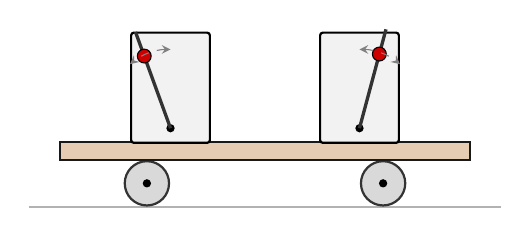
\begin{tikzpicture}[
    scale=1, transform shape,
    >=stealth,
    % Styles for the components
    roller/.style={circle, draw=black!80, fill=gray!30, thick, minimum size=16pt},
    board/.style={rectangle, draw=black!90, fill=brown!40, thick, minimum size=6pt},
    metronome/.style={rectangle, draw=black, fill=gray!10, thick, rounded corners=1pt},
    bob/.style={circle, fill=red!80!black, draw=black, minimum size=5pt, inner sep=0pt}
]

    % =========================================================================
    % 1. THE BASE: ROLLER CYLINDERS & COUPLING MOTION
    % =========================================================================
    % Ground line
    \draw[thick, gray!60] (-3, -0.3) -- (3, -0.3);

    % Two Cylindrical Rollers
    \node[roller] (left_roll) at (-1.5, 0) {};
    \node[roller] (right_roll) at (1.5, 0) {};
    
    % Tiny center dots for the cylinders
    \fill[black] (left_roll.center) circle (1.5pt);
    \fill[black] (right_roll.center) circle (1.5pt);

    % Coupling horizontal motion arrows for the board/rollers
    \draw[<->, line width=1pt, gray!80] (-2.2, 0.4) -- (-1.7, 0.4);
    \draw[<->, line width=1pt, gray!80] (1.7, 0.4) -- (2.2, 0.4);

    % =========================================================================
    % 2. THE COUPLING BOARD
    % =========================================================================
    % Stretches across both rollers
    \node[board, minimum width=5.2cm, anchor=south] (the_board) at (0, 0.28) {};


    % =========================================================================
    % 3. METRONOME 1 (Left Side - Tilted Left)
    % =========================================================================
    \begin{scope}[shift={(-1.2, 0.5)}]
        % Base/Body housing
        \node[metronome, minimum width=1.0cm, minimum height=1.4cm, anchor=south] (m1) at (0,0) {};
        
        % Pivot point location
        \coordinate (p1) at (0, 0.2);
        \fill[black] (p1) circle (1.5pt);
        
        % Long Pendulum Bar (Tilted left by 20 degrees)
        \draw[line width=1.2pt, draw=black!80] (p1) -- ++(110:1.3) coordinate (tip1);
        % Weighted Bob
        \node[bob] at ($(p1)!0.75!(tip1)$) {};
        
        % Motion arc indicator
        \draw[<->, dashed, thin, gray] (0, 1.2) arc (90:130:0.8);
    \end{scope}


    % =========================================================================
    % 4. METRONOME 2 (Right Side - Tilted Right)
    % =========================================================================
    \begin{scope}[shift={(1.2, 0.5)}]
        % Base/Body housing
        \node[metronome, minimum width=1.0cm, minimum height=1.4cm, anchor=south] (m2) at (0,0) {};
        
        % Pivot point location
        \coordinate (p2) at (0, 0.2);
        \fill[black] (p2) circle (1.5pt);
        
        % Long Pendulum Bar (Tilted right by 15 degrees)
        \draw[line width=1.2pt, draw=black!80] (p2) -- ++(75:1.3) coordinate (tip2);
        % Weighted Bob
        \node[bob] at ($(p2)!0.75!(tip2)$) {};
        
        % Motion arc indicator
        \draw[<->, dashed, thin, gray] (0, 1.2) arc (90:50:0.8);
    \end{scope}

\end{tikzpicture}
\caption{\textbf{Synchronization of metronomes.}
Illustration of an experiment consisting of two metronomes with different initial conditions and natural frequencies, on top of 
a board which is supported by cans. After some time, the metronomes synchronize.}
\label{fig:metronomes}
\end{figure}

We replaced the spins in a magnetic phase by the chirality of oscillators in a metamaterial. 
As a result, we obtained a set of interacting autonomous oscillators. %[explain more?]
These systems exhibit collective behaviour like synchronization, wave coarsening \cite{veenstra} 
and chaos, in different regimes. %[cite people, Jonas]
The most beautiful example of synchronization is placing two (or more) metronomes on a board \ref{fig:metronomes}. 
The board is supported by cans. 
The metronomes can have different initial conditions and different natural frequencies, and yet after some time 
they end up synchronizing \cite{PantaleoneSync}. 
The same phenomenom is responsible for fireflies \cite{fireflies}, circadian rhythm \cite{circadian} and many other examples. 
When oscillators oscillate with the same frequency, but with an arbitrary phase difference, it is called phase locking or synchronization. 
If the oscillators have a constant phase difference of $\pi$ or 180º, we refer to it as anti-phase synchronization. 
And if the oscillators oscillate with the same frequency and same phase, then it is called in-phase synchronization. 
Along the thesis, we mainly encounter in-phase synchronization. For convenience, we call it simply synchronization.
We specify when the phase difference is nonzero. 

There are three requirements for synchronization: the individual units must be autonomous oscillators, they must interact and their
individual parameters are similar to each other. The metronomes are autonomous oscillators, 
they interact throught the structure of the board and cans, and their natural frequencies must be sufficiently similar 
to display synchronization. 
The non-reciprocal units we introduced before trace out limit cycles and thus behave like two autonomous oscillators. 
They interact mechanically and weakly (see details in section \ref{sec:methods}). 
Again, if the individual parameters are similar, these units will synchronize too. 

The dynamics of limit cycles can be separated into two components. There is the amplitude and the phase. 
There are two types of Lyapunov exponents %eigenvalues of the Jacobian 
of the dynamical system. Most of them are negative, and they 
correspond to the stability of the limit cycle under perturbations in the amplitude. Though at least one of the eigenvalues 
is zero. It corresponds to phase shifts of the limit cycle trajectory. The fact that the eigenvalue is zero means the 
phase is neutral under phase perturbations. The phase shifted trajectory is still the limit cycle solution. As a consequence, 
the global phase of the limit cycle is not important. %, since one can just shift the phase effortlessly.
Since the phase grows with time, we can make time shifts that result in choosing the specific value of the phase desired. 
For weak interactions between units, the amplitude 
remains fixed to a constant value. They play no role in the dynamics. The only relevant degrees of freedom then are the phases. 
This dimensionality reduction in the degrees of freedom is sometimes called the phase dynamics approximation. 

We illustrate the simplest example of synchronization. Consider two identical non-reciprocal oscillators coupled together weakly, 
so that they still follow limit cycles. Therefore, the dynamics is described by the phases of the oscillators. 
When uncoupled, the oscillators have natural frequencies $\omega_1$ and $\omega_2$. 
Since the global phases are unimportant, the interaction terms must depend on the phase difference $\Delta\phi = \phi_2 - \phi_1$. 
The interaction might be a very complicated function of $\Delta\phi$. 
Nevertheless, it needs to be $2\pi$-periodic in the phase difference $\Delta\phi$. Therefore, we can expand it as a Fourier series. 
\begin{equation}
    H(\Delta\phi) = a_0 + \sum_{n=1}^\infty \left(a_n\cos{n\Delta\phi} + b_n\sin{n\Delta\phi}\right)
\end{equation}
%If the oscillators are synchronized $\Delta\phi=0$, we expect the interactions to vanish 
There are more constraints on the interaction $H(\Delta\phi)$. The actual mechanism carrying out the interaction 
in the experiments is a viscoleastic band. The mechanism is reciprocal and satisfies Newton's third law of action and reaction. 
The interaction that the first oscillator feels is exactly the opposite to the one the second one feels. 
The interaction terms must be opposite of one another: $H_1(\Delta\phi) = -H_2(\Delta\phi) = H(\Delta\phi)$. 
They must also conserve the symmetry exchanging the labels of the oscillators $1\leftrightarrow2$. 
This transformation has two effects on the equations. First, it exchanges $H_1\leftrightarrow H_2$, or more precisely, 
$H\leftrightarrow -H$. Second, the phase difference changes sign, because we have swapped the order: $\Delta\phi\rightarrow-\Delta\phi$.
Since this relabeling should not have any effect on the dynamics, we find the condition $-H(-\Delta\phi)=H(\Delta\phi)$. 
The interaction must have odd parity to respect the reciprocity between identical oscillators. 
Therefore, all the even terms in the Fourier series vanish. We are only left with sine terms. 
Moreover, as the interaction is weak, we can approximate the interaction term by its leading order term: $\sin{\Delta\phi}$. 
Higher order terms oscillate very fast and average out to zero. 
We arrive at the Kuramoto model \cite{kuramoto} of two oscillators:
\begin{align}
    \dot{\phi}_1 &= \omega_1 + K \sin(\phi_2 - \phi_1) = \omega_1 + K \sin(\Delta\phi) \label{eq:Kuramoto_1}\\
    \dot{\phi}_2 &= \omega_2 + K \sin(\phi_1 - \phi_2) = \omega_2 - K \sin(\Delta\phi) \label{eq:Kuramoto_2}.
\end{align}
As the global phase is unimportant, we can focus on the dynamics of the phase difference.
The equation is obtained by subtracting \eqref{eq:Kuramoto_1} and \eqref{eq:Kuramoto_2}. 
The result is the Adler equation:
\begin{equation}
    \frac{d \Delta \phi }{dt} = \Delta \omega - 2 K \sin(\Delta \phi).
    \label{eq:adler}
\end{equation}
The first term in the RHS is the detuning or mismatch of the natural frequencies. The second term is the 
leading order contribution of the interactions. 
Synchronization occurs when the phases are locked together: $\frac{d \Delta \phi }{dt}=0$. In other words, 
synchronization solutions are given by the zeros of the RHS of \eqref{eq:adler}. The Adler equation 
predicts two regimes. If $\Delta \omega <2K$, the function on the RHS has zeros and the oscillators synchronize. 
If $\Delta \omega >2K$, the function has no zeros and the oscillators do not synchronize. The system then 
exhibits beating, phase drift or chaos. 

\section{Methods}
\label{sec:methods}

\subsection{Actuators}
\label{subsec:actuators}

To replace spin by oscillator chirality, we use two actuators coupled non-reciprocally. 
We use custom-made voice coil linear actuators, shown in figure \ref{fig:actuator_ronald}.
The actuators have several components. They have a passive elastic structure, which is black and orange 
in figure \ref{fig:actuator_ronald}, that makes it behave like a damped spring. 
We can also program custom forces into the actuator. The actuator uses the magnetic Lorentz force to   %$F=ILB\sin{\Th}=kI$/
displace itself, namely $\vec{F}=L\vec{I}\times \vec{B}$. Therefore, the actuator functions thanks to magnetic field and an electric current. 
The magnetic field $B$ is generated by a cylindrical iron permanent magnet in the center of the actuator.
The current is generated externally with a power supply. The current intensity $I$ goes through a copper coil that surrounds the magnet, 
which has length $L$. The magnetic field lines extend outward radially $\vec{B}=B\hat{r}$, 
while the current winds in the azimuthal direction $\vec{I}=I\hat{\phi}$.
As the magnetic field lines cross the coil perpendicularly, the Lorentz force generated is directed 
along the cylinder: $\vec{F}=LI\hat{\phi}\times B\hat{r}=LIB\hat{z}$.
For a given actuator, the factor $k=LB\sin{\Th}$ is fixed. The only parameter we control is the current. 
The actuator feels a force linear in the current intensity $I$ going through the coil. 
Reversing the direction of the current also reverses the direction of the force. 
The coil is fixed with a 3D-printed passive structure of Tough1500 resin. 
The force produced moves the ion magnet along the axial coordinate. The spring structure 
maintains the magnet aligned with the coil. When the magnet is displaced, the spring structure also compresses. 

We are interested in implementing odd elasticity, a force that depends on the position. 
The actuators use a Texas Instruments linear Hall effect sensor (DRV5057A3) to measure the position of the magnet. 
As the name suggests, the sensor employs the Hall effect to measure magnetic fields as Hall voltages. 
Since the magnet is displaced back and forth linearly, the Hall sensor can be used to measure those voltage changes, 
and transform them into displacements of the position. 
We can program odd elasticty into the actuators, by connecting them to a custom Printed Circuit Board (PCB) 
with a simple microprocessor (RP235x). The PCB reads out the Hall sensors at \SI{2}{kHz} 
and calculates the current input to the coils at \SI{1}{kHz}. The firmware is also custom. 

\subsection{Coupling with neighbours}
\label{subsec:coupling}
All the actuators move back and forth in one direction, which we will denote the $x$ direction. 
We will couple the actuators to their neighbours via a viscoelastic band. The coupling strength 
is denoted by $k_b$. Note that the coupling occurs in the directions perpendicular to 
the motion of actuators, so in the $y$ and $z$ direction. Consider the simplest case in which we have 2 
actuators coupled by a viscoelastic band in the $y$ direction. 
% do diagram with tikz
The distance between the two actuators is $l$. When one of the actuators moves in the $x$ direction, 
it stretches the viscoelastic band, which creates a restoring force in the $x$ direction. Let 
$\varDelta x = x_2 - x_1$ be the difference in the $x$ positions of the two actuators with 
respect to their equilibrium position. For a displacement $\varDelta x$, the viscoelastic band stretches 
from a distance $l$ to a distance $d = \sqrt{l^2 + \varDelta x^2}$. The restoring force 
acting in the first actuator is given by Hooke's law as $\vec{F} = k_b (\vec{d} - \vec{l})$. 
But keep in mind that the actuators can only move in the $x$ direction, so they only feel 
the $x$ component of the force, which is multiplied by $\sin \theta$:
\begin{equation}
    F_x = k_b (d - l) \sin \theta = k_b (\sqrt{l^2 + \varDelta x^2} - l) \frac{\varDelta x}{\sqrt{l^2 + \varDelta x^2}} 
    = k_b \varDelta x \left(1 - \frac{l}{\sqrt{l^2 + \varDelta x^2}}\right) 
    \label{eq_geometric_stiffening}
\end{equation}
where $\theta$ is the angle between the viscoelastic band and the $y$ axis. One would expect that the coupling 
is linear in $\varDelta x$ due to Hooke's law. However, the geometry of the coupling, in which the 
actuator displacement and the viscoelastic band are not collinear, leads to the appearance of a 
nonlinear factor in the coupling. This is known as geometric stiffening. 

We can consider the limiting cases of equation \eqref{eq_geometric_stiffening}. If the $x$ displacements are 
very large in comparison with $l$, then the nonlinear factor vanishes and the force becomes linear in the displacement. 
If the $x$ displacements are small with respect to $l$, then we can Taylor expand the nonlinear factor as
\begin{equation}
\left[1+ \left(\frac{\varDelta x}{l}\right)^2\right]^{-1/2} \approx 1 - \frac{1}{2}\left(\frac{\varDelta x}{l}\right)^2 + \mathcal{O}\left(\left(\frac{\varDelta x}{l}\right)^4\right).
\end{equation} 
In that case, the force acting on the actuator in the $x$ direction is approximately given by
\begin{equation}
    F_x \simeq  k_b \frac{\varDelta x ^3}{l^2}, \; \text{for} \; \varDelta x \ll l.
    \label{eq_neighbour_coupling_approx}
\end{equation}
In our setup, the amplitude of each actuator is at most $\SI{3}{mm}$. As a consequence, $\varDelta x < \SI{6}{mm}$. 
The smallest distance in $y$ direction between actuators is $l = \SI{35}{mm}$. 
This means we are in the regime of small displacements, and we need to use equation \eqref{eq_neighbour_coupling_approx}.
Note that this equation is not linear in $\varDelta x$, but it is cubic. We expect the coupling in the direction perpendicular 
to displacement to be smaller than in the collinear case. It makes sense because the cubic term is smaller than the 
linear term, and so the coupling is weaker than ordinary Hooke's law. 
An additional thing to note is that we can recover the linear coupling by pre-tensioning the viscoelastic band. 
In the experimental setups, we use the band to keep the actuators straight and keep them from being pulled down by gravity. 
So all the actuators move the band in the same way, and the band remains unstretched. To conclude, the coupling between 
neighbour actuators is given by formula:
\begin{equation}
    F = \frac{k_b}{2l^2} (x_2 - x_1)^3.
\end{equation}

\subsection{Experimental setup}
\label{subsec:experimental}

\begin{figure}[htbp]
  \centering
  \begin{subfigure}[b]{0.48\textwidth}
    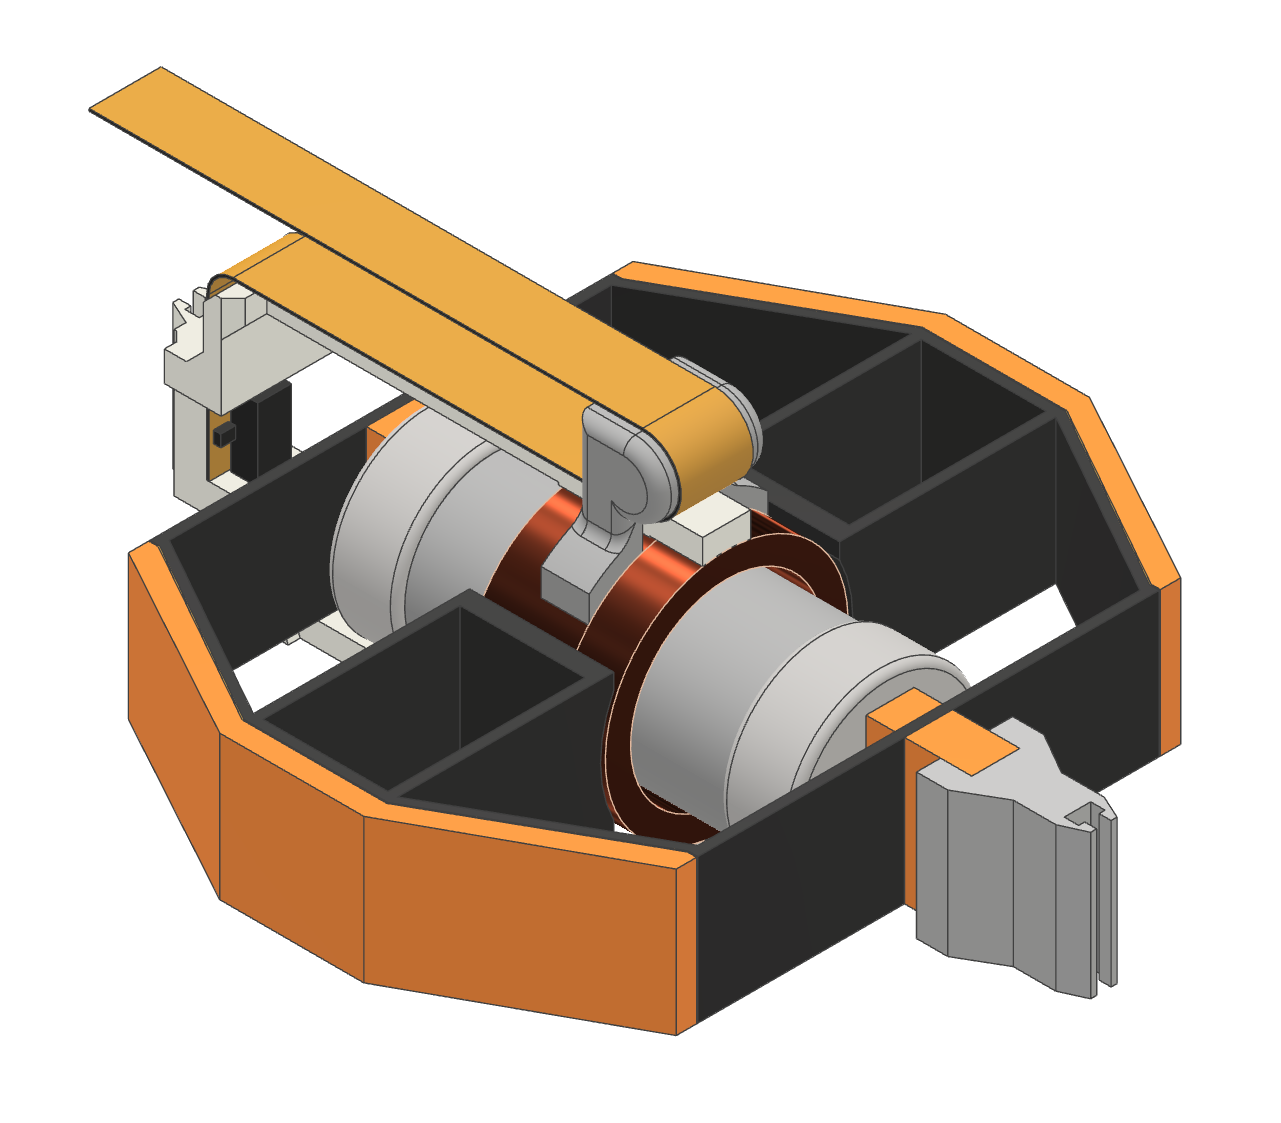
\includegraphics[width=0.8\textwidth]{actuator_ronald.png}
    \caption{}
    \label{fig:actuator_ronald}
  \end{subfigure}
  \hfill
  \begin{subfigure}[b]{0.48\textwidth}
    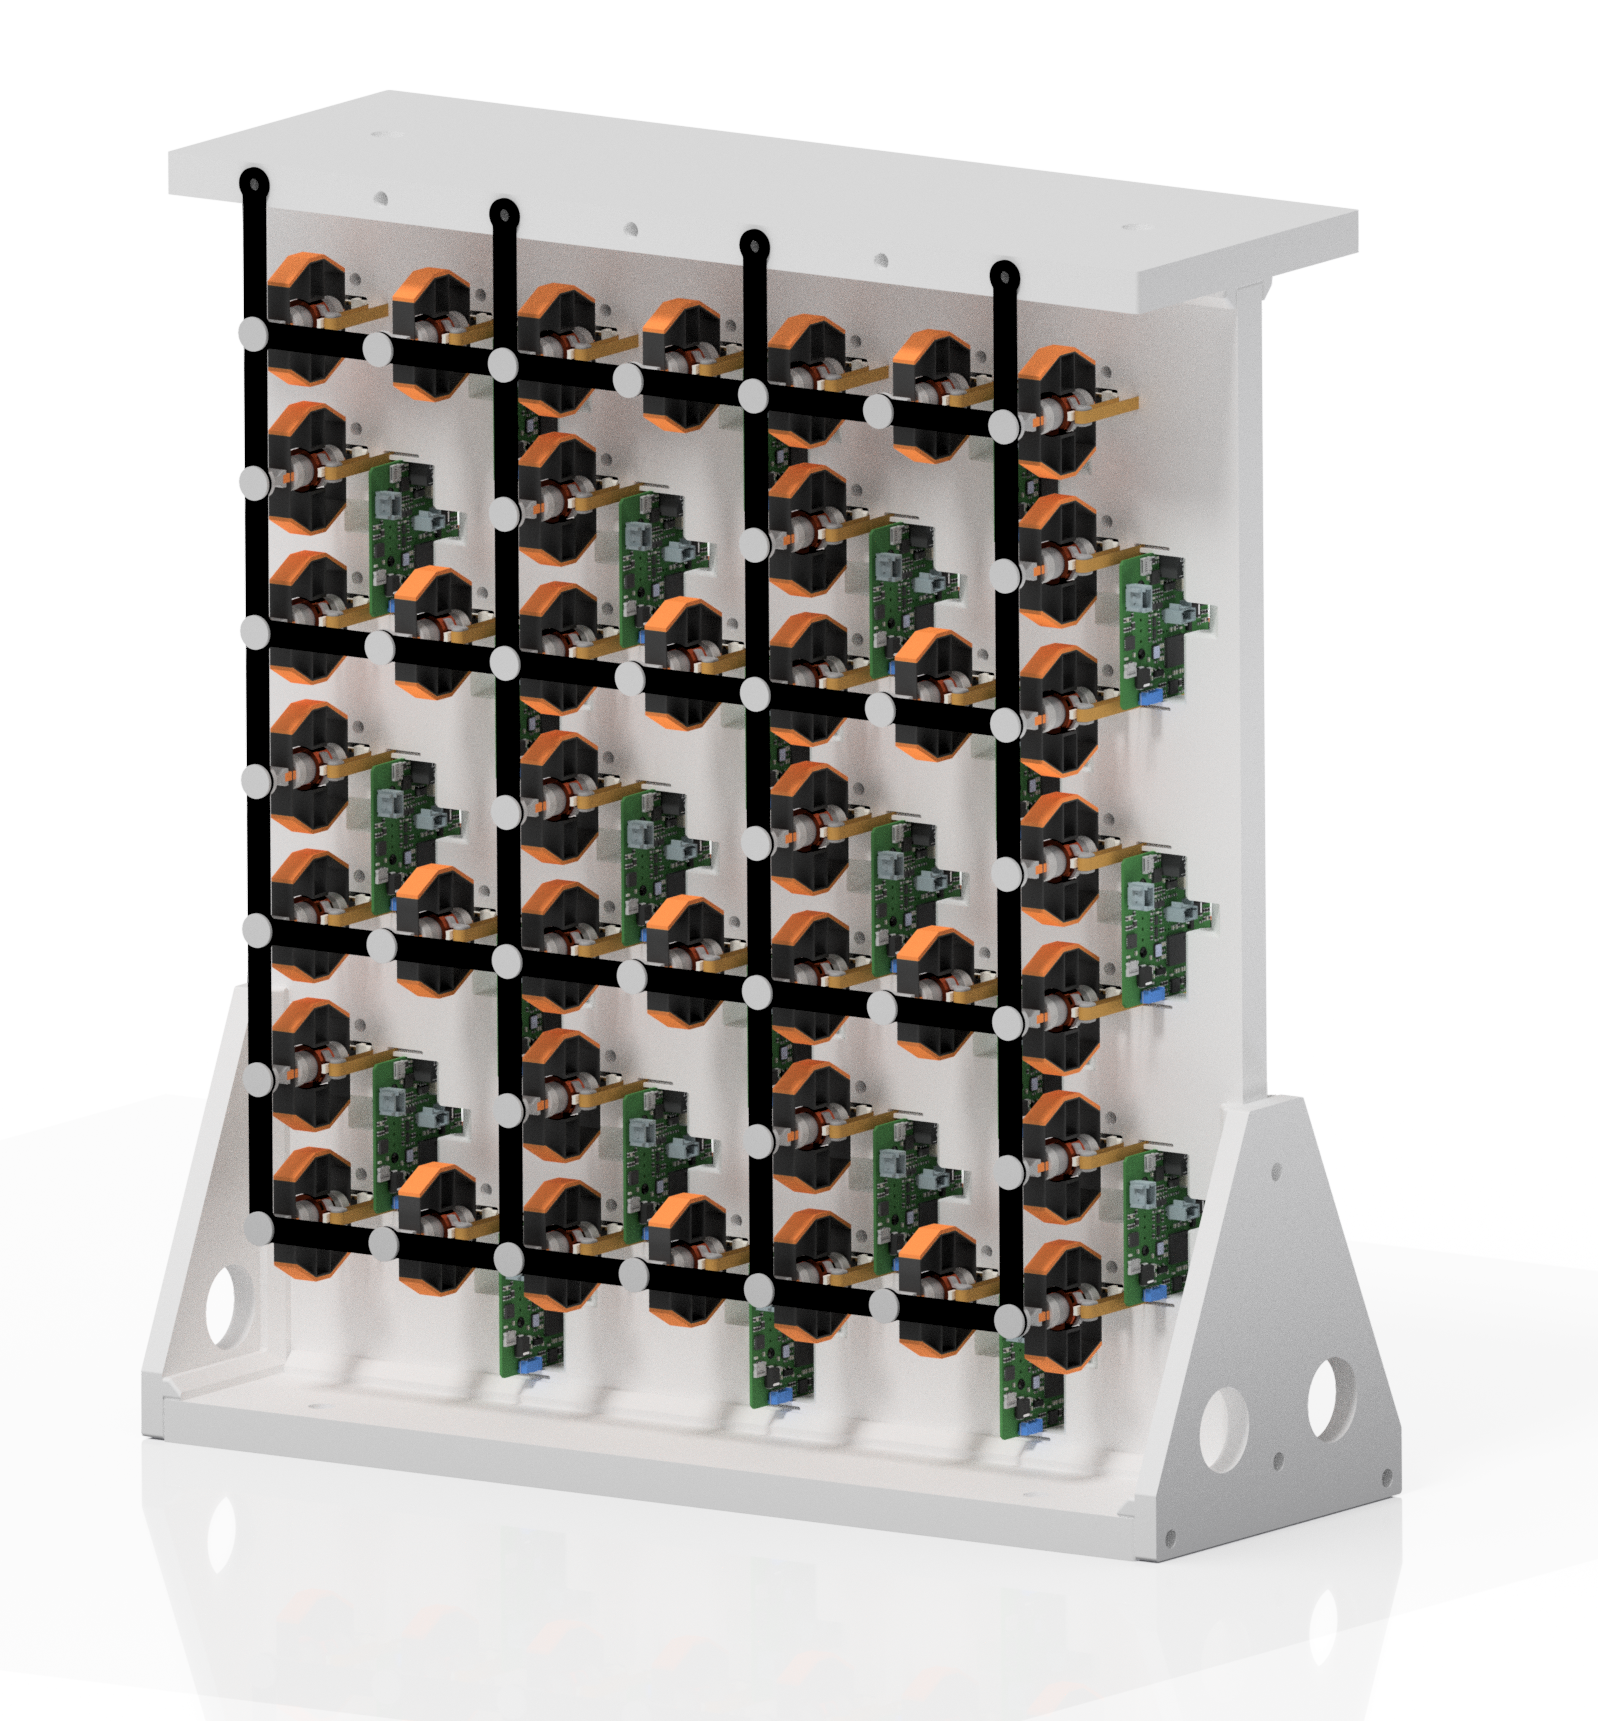
\includegraphics[width=0.8\textwidth]{setup_ronald.png}
    \caption{}
    \label{fig:setup_ronald}
  \end{subfigure}
  \caption{\textbf{Actuator and experimental apparatus.} 
  \textbf{\ref{fig:actuator_ronald}} Voice coil linear actuator with a cylindrical iron magnet, a copper coil that winds around it, 
  and a elastic structure that keeps the former and the latter aligned. The actuator operates due to the magnetic Lorentz force.
  A current is provided through the coil (angular), which interacts with the radial magnetic field 
  to yield a displacement in the axial ($z$) direction.
  \textbf{\ref{fig:setup_ronald}} Mechanical Lieb lattice made out of coupled actuators. The apparatus has two layers of actuators 
  arranged in a Lieb lattice. The two layers are separated by a wall, to which the actuators are fixed. 
  The interaction within the layers is through viscoleastic bands. The interaction between the layers is odd elasticity, only 
  between mirror actuators. }
  \label{fig:experimental_setup}
\end{figure}

The experimental setup is made up of two 2D layers of actuators. The two layers are separated by a wall, where 
we attach the actuators. There are two types of interactions between the actuators. First, there is the odd elasticity 
we already introduced in \ref{subsec:non-reciprocity}. This interaction is programmed into the PCB connecting the two actuators.
Each actuator is placed to one side of the wall. Altogether they form a non-reciprocal unit. The second type of interaction 
consists of a viscoelastic band attached to the ends of the actuators, which we introduced in section \ref{subsec:coupling}.
The band is fixed at the top of the wall structure to counteract the effect of gravity. However, it is fixed 
neither at the bottom nor on the sides. 

The actuators making up the layers on either side of the wall interact through the viscoelastic band. The interaction 
between actuators on different sides of the wall is exclusively odd elasticity. The setup can also be interpreted as 
one 2D layer of non-reciprocal units. 
We can arrange the actuators in different configurations. This allows the study of systems with different symmetries and dimensions. 
Some examples are 1D chains, cross cells and the altermagnet $C_4\mathcal{T}$ symmetry of the Lieb lattice. 
Besides the way we place the actuators and couple them, the only parameter we control is the activity $k_a$ of the actuators.


In order to carry out measurements, we use a set of high-speed cameras called Qualisys Arqus 5 to track the position of the actuators.
The cameras record the position in 3D space, sampling at a rate of $f_s = \SI{500}{Hz}$. %[what is the precision?]
We sometimes calculate the oscillation frequency by performing a Fourier transform. The precision of the frequency 
results depends on the recording time of the experiment, assuming the system is in the steady state. 
As the frequency resolution of the Fourier transform is $\varDelta f = \frac{f_s}{N} = \frac{f_s}{f_s T} = \frac{1}{T}$.
In the previous formula, $N=f_s T$ is the total number of samples taken and $T$ is the total time of recording. 
Therefore, we increase the precision of the measurements by recording for longer times. 

% Hence we chose a value of $T=\SI{10}{s}$. 
% Let’s start first with only one unit, that is, 
% 2 non-reciprocal actuators. In the following measurements, we varied the activity parameter $k_a$ 
% of the single unit. When the unit undergoes limit cycles, we record the position of the actuators for 10 
% seconds, sampling at a rate of $f_s = \SI{500}{Hz}$. We are interested in the amplitude and frequency of oscillation 
% of the limit cycles. Note that the frequency is obtained by performing a Fourier transform and its accuracy is 
% determined by how long we record: $\varDelta f = \frac{f_s}{N} = \frac{1}{T}$. In the previous formula, $N$ 
% is the total number of samples taken and $T$ is the total time of recording. Therefore, we increase the precision 
% of the measurements by recording for longer times, hence the chosen value of $T=\SI{10}{s}$. 


% We connect the springs electronically between each other and to a power source. Using 
% PCBs (printed circuit boards), we can program odd-elasticty / non-reciprocity in the coupling between springs.
% In order to have nontrivial steady-state dynamics, we need the springs to oscillate and that requires overcoming friction. 
% Here is where the non-reciprocal coupling comes in handy. It will allow the springs to carry out self-sustained oscillations 
% in the form of limit cycles. The system can then be easily analized experimentally in the steady state.
% Describe the models used: one site, two site, ladder/chain 1d strip, bilayer Lieb lattice, 
% Rupesh's levers model.

\subsection{General theoretical procedure}
\label{subsec:theoretical_procedure}
%[maybe move stuff from MSE about hamiltonian]

As we have mentioned, we want to study systems made of classical springs with different geometries. 
%The end goal is to build a system with the altermagnetic symmetry and see if its properties coincide with those of altermagnets.
In this section we outline the steps involved in the theoretical description of a general system. 

The first step is to write down the equations of motion for the system. To do so, we use Newton's second law 
and add all relevant forces acting on the system. The forces we consider are: linear elastic stiffness of the spring, 
damping force due to the spring's friction, nonlinear saturation of the spring, coupling to neighbours via a viscoelastic band and coupling to 
neighbours via odd elastic interactions. All the force terms except the latter can be realized in experiments mechanically. For the latter, 
we need to plug energy into the system.  
If $N$ is the number of springs of our system, we will have a system of $N$ coupled second-order ordinary differential equations. 
Note that the number of degrees of freedom is $2N$, because we have the position and velocity of each spring. 

The second step is to perform an asymptotic expansion of the solution. Solving the whole system is very difficult. 
One way to simplify the problem is to identify which force terms are the strongest and which are the smallest. 
We can treat the smaller terms as perturbations to the strongest one. This divides the problem into solving the 
unperturbed system, without the small perturbations, and then adding the effect of the perturbations. 
We denote the smaller terms by adding a factor of $\epsilon \ll 1$ in front of them. 
Intuitively, the strongest term will have a much faster timescale than the smaller ones. The springs will 
exhibit several of these timescales in their periodic motion. The asymptotic expansion allows us to study the 
different timescales separately. This can be done in practice in two ways. The first is the method of averaging. 
This method removes the fast timescale by averaging over its period. Then, the resulting equations 
describe the slow dynamics, and one can then solve them. 
The second way is the multiple scale expansion, which is more rigorous but uses the same idea. 
In the next section \ref{subsec:mse}, we show the steps of the method for a simple example. The method introduces 
different time variables, each denoting one of the timescales. We restrict ourselves to two timescales. 
The problem is then divided into two equations with different timescale magnitudes, and the ODE has transformed into a PDE.
Then, one can solve the fast timescale equation (order $\epsilon^0$). Notice that the two constants of integration from solving the 
partial differential equation now become coefficients depending on the slow time variable. These coefficients 
are complex if one considers as basis a Fourier series: $e^{in\omega t}$. It is also important to note 
that the couplings in the classical equations of motion are real, which constrains the two coefficients 
to be complex conjugates of each other.  
One then uses that solution to solve the slow timescale equation (order $\epsilon$). The slow timescale 
equation contains secular terms, which are terms that grow unboundedly. They arise from the asymptotic expansion and 
from the fact that the fast timescale solution contains free parameters to be determined. We can choose 
the free parameters such that the secular terms vanish. This is called the solvability condition, and 
it comes from the Fredholm alternative theorem in analysis. It states that 
a linear inhomogeneous equation has a solution if and only if the inhomogeneous term is orthogonal to the null 
space of the adjoint operator of the differential equation. The solvability condition leads to 
new equations that govern the slow time dynamics of the free parameters. These equations are called amplitude equations, 
modulation equations, envelope equations or Stuart-Landau equations. 
So we have rewritten the original degrees of freedom  $(x,\xd)$ in terms of a complex valued coefficient we denote by $A(T)$.
And we have replaced the classical equations of motion by the amplitude equations for $A(T)$. 
The important difference is that $A(T)$ only contains the slow timescale dynamics, 
while the fast timescale dynamics is encoded in the basis functions $e^{in\omega t}$.
Moreover, the amplitude equations are first order ODEs, while the original equations of motion were second order ODEs.
The reason for this is the relation between the position and velocity in an oscillatory system, which is a factor $i \omega$.
Therefore, the linearized dynamics are described by an evolution matrix analogous to the Hamiltonian of the Schrödinger 
equation. Studying its spectrum and eigenvectors gives us useful information about the system. We actually 
compared these evolution matrices with tight-binding quantum Hamiltonians, to get intuition. 
In the next section, we will see how to apply the multiple scale expansion to a simple example, the weakly damped harmonic oscillator.
Note that $\omega$ is just a parameter that we can choose, and it is usually chosen to be the natural frequency of the unperturbed system.


The third step is to replace the complex modulation coefficients by their amplitude/radius and phase: $A(T) = R(T)e^{i\Th(T)}$. 
This step again separates the dynamics into 2 equations, one for the radius and one for the phase. Thus there is one radius and 
one phase equation for each spring.  


The next step is to reduce the number of equations. We can do so by noting that the dynamics of the springs are stable limit cycles (in general). 
They are characterized by the fast decay of perturbations in the amplitude/radius of oscillation. 
In rigorous terms this means that the Lyapunov exponents of the amplitude components are negative, and perturbations 
decay exponentially fast. However, limit cycles have a zero mode, which corresponds to phase changes. Perturbations in the 
phase neither grow nor decay. The Lyapunov exponent associated to the phase is zero. Therefore, 
deviations in the radius/amplitude are much smaller than deviations in the phase. One can then take the 
phase dynamics approximation, which consists in assuming that the radius/amplitude of the limit cycle is (periodically) constant.
In other words, the shape of the limit cycle is fixed. One ends up with a system of $N$ coupled first order ODEs 
for the phase of each spring. 


%[also mention the case for "infinite"/periodic system, use fourier space]
One can also carry out the procedure for a system with periodic boundary conditions. With these boundaries it is easier 
to study the infinite size limit.
The way to go is to do a Fourier transformation to momentum space. The difference is one is now working with 
the momentum basis, and the displacements are not labelled by position, but by momentum. Then one can follow the same steps as before.

\subsection{Multiple scale expansion}
\label{subsec:mse}
% In this section, I should also add some details from Pikovsky section 7.1 and 7.2. Also,   DONE
%the rigorous way to obtain the amplitude equation by setting the secular terms to zero is called the solvability condition, DONE
% and it is explained in detail in Kuramoto's book.  DONE

 The method of multiple scales is a powerful technique for analyzing nonlinear ordinary differential equations that exhibit dynamics on widely separated timescales. To illustrate the approach, consider the weakly damped harmonic oscillator described by the equation
\[
\ddot{x} + x + 2\varepsilon \dot{x} = 0,
\]
where $\varepsilon \ll 1$ represents a small dimensionless parameter quantifying the weak damping. A naive perturbation approach would seek an approximate solution as a power series expansion in $\varepsilon$:
\[
x(t) = x_0(t) + \varepsilon x_1(t) + \mathcal{O}(\varepsilon^2).
\]
Substituting this ansatz into the governing equation yields the hierarchy of equations
\[
[\ddot{x}_0 + x_0] + \varepsilon[\ddot{x}_1 + x_1 + 2\dot{x}_0] + \mathcal{O}(\varepsilon^2) = 0.
\]
Solving these equations order by order gives the approximate solution
\[
x(t,\varepsilon) = \sin t - \varepsilon t\sin t + \mathcal{O}(\varepsilon^2).
\]

However, this approximation becomes invalid for times $t > \mathcal{O}(1/\varepsilon)$ due to the presence of 
secular terms that grow without bound. To obtain an approximation valid on longer timescales, we introduce two 
independent time variables: the fast time $\tau = t$ and the slow time $T = \varepsilon t$. The solution is 
then sought as a function of both timescales:
\[
x(t,\varepsilon) = x_0(\tau,T) + \varepsilon x_1(\tau,T) + \mathcal{O}(\varepsilon^2).
\]

The time derivative transforms according to the chain rule:
\[
\frac{d}{dt} = \partial_\tau + \varepsilon \partial_T,
\]
so that
\[
\dot{x} = \partial_\tau x_0 + \varepsilon(\partial_T x_0 + \partial_\tau x_1) + \mathcal{O}(\varepsilon^2).
\]

At leading order ($\mathcal{O}(\varepsilon^0)$), we obtain
\[
\partial_{\tau\tau}x_0 + x_0 = 0,
\]
which admits the general solution
\[
x_0(\tau,T) = A(T)\sin\tau + B(T)\cos\tau,
\]
where the coefficients $A$ and $B$ are allowed to vary slowly with $T$. At next order ($\mathcal{O}(\varepsilon)$), we find
\begin{equation}
    \partial_{\tau\tau}x_1 + x_1 = -2(\partial_{T\tau}x_0 + \partial_\tau x_0).
    \label{eq_mse_order_eps}
\end{equation}

To avoid secular terms that would render the perturbation expansion invalid for $t \sim 1/\varepsilon$, 
we require the right-hand side to be equal to zero. %orthogonal to the homogeneous solutions. 
This is called the solvability condition. The underlying reason behind it is a mathematical theorem 
called the Fredholm alternative. It states that there are two possibilities or alternatives 
for a general operator. If the homogeneous equation of the aforementioned operator only has the trivial 
solution, it means that the operator is nonsingular and the inhomogeneous equation will have a unique solution for any 
source term. The alternative is that if the homogeneous equation has nontrivial solutions, then 
the operator is singular, and there is no guarantee of solutions for a general source term. In the former case, 
the nullspace of the operator is trivial, it contains only the zero vector. 
The dimensionality of the nullspace and range of an operator are related and have to sum to the 
dimension of the vector space. As a consequence, the range of the operator in the first case 
is the whole vector space, and that includes any source term.
If the nullspace has nonzero dimensionality, that means that the range doesn't include the whole vector space. 
In other words, there are some source terms for which the inhomogeneous equation has no solution. Mathematically, those 
terms form the nullspace of the adjoint operator. We can call them homogeneous adjoint solutions. 
If we require the equation to have a solution, we must avoid them. The projection of the source term with the 
homogeneous adjoint modes must be set to zero. In physics terms, the nontrivial homogeneous solutions are plane waves with the 
frequency of the operator. That is precisely the resonant frequency of the system. If one adds a resonant-frequency source term
then the system blows up. That is precisely what happens in equation \eqref{eq_mse_order_eps}. 
In the example, the operator is the harmonic oscillator and $x_0$ is the solution to the homogeneous equation, i.e. the equation 
at order $\mathcal{O}(\varepsilon^0)$. The equation at order $\mathcal{O}(\varepsilon)$ is again the same harmonic oscillator 
for $x_1$, with some additional source terms linear in $x_0$. Thus, the source terms oscillate with the resonant frequency, and they 
are called secular. For the solution to be well-defined, periodic and bounded, the secular terms must cancel out, yielding 
the solvability condition. 
% The homogeneous adjoint modes are plane waves with opposite frequency. 

This solvability condition yields the differential equations
\[
A' + A = 0 \quad \text{and} \quad B' + B = 0,
\]
where primes denote differentiation with respect to $T$. 
These equations are called modulation equations, as they govern the slow evolution of the oscillation amplitude and phase. 
They are first order coupled linear ordinary differential equations that can be solved straightforwardly. 
However, we will gain more insight by writing them as Schrödinger-like equations. We can do so by writing the equations 
in matrix form, and multiplying by $i$:
\begin{equation}
    i\begin{pmatrix}
    A' \\ B'
    \end{pmatrix}
    =
    \begin{pmatrix}
    -i & 0 \\
    0 & -i
    \end{pmatrix}
    \begin{pmatrix}
    A \\ B
    \end{pmatrix}
\end{equation}
The matrix on the right-hand side can be interpreted as an effective non-Hermitian Hamiltonian describing 
the slow dynamics of the amplitudes $A$ and $B$. All the system's properties are encoded in this matrix. 
Therefore, in general we will compute the eigenvalues and eigenvectors of such effective Hamiltonians 
and interpret them to understand the long-time behaviour of the original system. The solution can be written as
a combination of the eigenmodes of the Hamiltonian, each evolving in time with a phase according to its eigenvalue $e^{-iEt}$.

Back to the example, the Hamiltonian in this case is $H=-i I$, where $ I$ is the identity matrix. Then, the 
eigenvalues are both $-i$, which have negative imaginary part. This means that both amplitudes decay exponentially in time.
The solutions are $A(T) = A_0 e^{-T}$ and $B(T) = B_0 e^{-T}$. Substituting back, we obtain the uniformly valid approximation
\[
x(t,\varepsilon) = e^{-\varepsilon t}(A_0\sin t + B_0\cos t) + \mathcal{O}(\varepsilon),
\]
which correctly captures the slow exponential decay of the oscillation amplitude. This example demonstrates the essential ideas 
of the multiple scales method, which can be extended to more complex nonlinear systems exhibiting multiple timescales.

\section{One non-reciprocal unit}
\label{sec:1unit}
In this section we implement mechanical spin or oscillator chirality using two linear actuators interacting non-reciprocally. We show the 
theoretical modelling first and afterwards the experimental results. 

\subsection{Theory}
\label{subsec:1unit_theory}

We consider the simplest model possible to replace spin: two linear actuators 
coupled non-reciprocally. We denote the two degrees of freedom as $x$ and $y$, which correspond to the displacement of the 
actuators from the equilibrium position. We choose the specific non-reciprocal interaction to be odd elasticity. %, as discussed in section . 
One can interpret the system as a 2D oscillator. 
The equations of motion are
    \begin{align}
        \xdd +k_0x +  \gamma \xd + k_cx^3 + k_ay = 0 \label{eq_1osc_x} \\ % %already defined later
        \ydd +k_0y +  \gamma \yd + k_cy^3 - k_ax = 0 \label{eq_1osc_y}
    \end{align}
%[should I add nonlinear cubic term to stabilize??]
where \( k_0 \) is the harmonic linear stiffness, \( \gamma \) is the damping coefficient, $k_c$ is a nonlinear saturation coefficient 
that stabilizes the dynamics, and \( k_a \) is the non-reciprocal coupling strength, also called the activity or gain. 
%The parameter \( \epsilon \ll 1 \) indicates that both damping and non-reciprocal coupling are weak perturbations to the harmonic oscillator.
There are different ways to analyse the system. One way is to plug in the plane wave ansatz 
\( x(t) = X e^{-iEt} \) and \( y(t) = Y e^{-iEt} \) in the linearized equations, and solve for the frequencies/energies $E$. 
Another method is to perform the multiple scale expansion, as explained in the section \ref{subsec:mse}.
    The energies of the linearized system are 
    \begin{align}
        \text{clockwise:} \; E_1 = -\frac{i}{2}\left(\gamma + \frac{k_a}{\sqrt{k}}\right), \label{eq_1osc_e1}\\ %
        \text{counterclockwise:} \; E_2 = \frac{i}{2}\left(-\gamma + \frac{k_a}{\sqrt{k}}\right), \label{eq_1osc_e2}
    \end{align}
    and the eigenvectors are 
    \begin{align}
        \text{clockwise} \; v_1 = \begin{pmatrix}
        1 \\ -i
        \end{pmatrix} \label{eq_1osc_v1} \\ %
        \text{counterclockwise} \; v_2 = \begin{pmatrix}
        1 \\ i
        \end{pmatrix} \label{eq_1osc_v2}.
    \end{align}
    On the one hand, $E_1$ has 2 eigenvectors in which the oscillator rotates clockwise in the plane. 
    What distinguishes these eigenvectors is their initial phase, basically a global phase. As the time evolution is given by the 
    phase factor $e^{-iEt}$, these modes are exponentially suppressed as time evolves.
    On the other hand, $E_2$ has 2 eigenvectos that rotate counterclockwise, each with a different initial phase. 
    Note that the energies are complex as a consequence of the abscence of energy conservation. 
    There are two regimes for the system described by equations \eqref{eq_1osc_x} and \eqref{eq_1osc_y}. 
    If $|k_a| < \gamma \sqrt{k}$, so for low values of activity, the energies have all a negative imaginary part. 
    This means that the oscillations of the actuators are exponentially damped, because friction dominates. The origin is a stable fixed point, 
    so the system becomes at rest and there is no motion. However, if the activity $|k_a|$ is increased, the system undergoes a supercritical 
    Hopf bifurcation. For $|k_a| > \gamma \sqrt{k}$, the origin is unstable and a stable limit cycle appears. The cubic 
    term $k_cx^3$ is necessary for the limit cycle to be stable. The sign of the activity $k_a$ determines the direction of 
    the limit cycle. If $k_a>0$, the limit cycle has counterclockwise direction, and if $k_a<0$, it has clockwise direction. 
    This feature can be seen in equations \eqref{eq_1osc_e1} and \eqref{eq_1osc_e2} by changing the sign of $k_a$. If the sign is changed, 
    the modes that can have the limit cycles, only for sufficiently large activity, are the ones corresponding to the clockwise chirality. 

    \begin{figure}[htbp]
        \centering
\begin{subfigure}[b]{0.58\textwidth}
    \begin{center}
            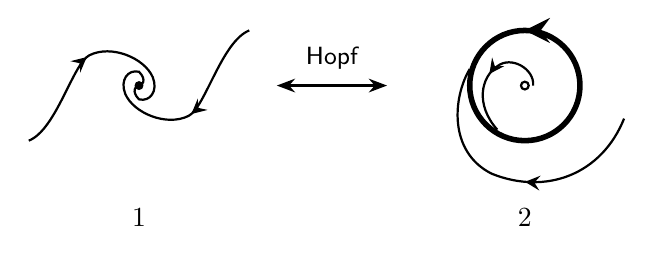
\begin{tikzpicture}[scale=0.7, >=Stealth]

    % =========================================================================
    % SUBFIGURE 1: Left Diagram (Stable Fixed Point)
    % =========================================================================
    \begin{scope}[shift={(0,0)}]
        % Trajectory from bottom-left, spirals into fixed point
        \draw[thick, flow=0.45]
          (-2.0,-1.0) .. controls (-1.5,-0.8) and (-1.2, 0.4) ..
          (-0.9, 0.55) .. controls (-0.5, 0.75) and ( 0.1, 0.5) ..
          ( 0.25, 0.15) .. controls ( 0.35,-0.1) and ( 0.2,-0.3) ..
          ( 0.0,-0.25) .. controls (-0.15,-0.1) and (-0.05, 0.0) ..
          (-0.02, 0.0);

        % Second trajectory from top-right, spirals into fixed point
        \draw[thick, flow=0.45]
          ( 2.0, 1.0) .. controls ( 1.5, 0.8) and ( 1.2,-0.4) ..
          ( 0.9,-0.55) .. controls ( 0.5,-0.75) and (-0.1,-0.5) ..
          (-0.25,-0.15) .. controls (-0.35, 0.1) and (-0.2, 0.3) ..
          ( 0.0, 0.25) .. controls ( 0.15, 0.1) and ( 0.05, 0.0) ..
          ( 0.02, 0.0);

        % Stable fixed point (filled dot)
        \filldraw (0,0) circle (2pt);

        % Subdiagram Label
        \node at (0,-2.4) {1};
    \end{scope}

    % =========================================================================
    % CONNECTING ARROW: Double-headed arrow with "Hopf" label
    % =========================================================================
    \draw[<->, thick] (2.5, 0) -- (4.5, 0) 
        node[midway, above=2pt, font=\small\sffamily] {Hopf};

    % =========================================================================
    % SUBFIGURE 2: Right Diagram (Limit Cycle) - Shifted by 7 units right
    % =========================================================================
    \begin{scope}[shift={(7,0)}]
        % Stable limit cycle (thicker, radius 1 cm)
        \draw[line width=2pt, flow=0.25] (0,0) circle (1.0cm);

        % Trajectory spiralling outward from near origin to limit cycle
        \draw[thick, flow=0.5]
          (0.15, 0.0)
          .. controls ( 0.18, 0.30) and (-0.25,  0.55) ..
          (-0.5,  0.35)
          .. controls (-0.80, 0.15) and (-0.90, -0.35) ..
          (-0.5, -0.80);   % ends near the circle r ≈ 1

        % Trajectory spiralling inward from outside to limit cycle
        \draw[thick, flow=0.45]
          ( 1.80,-0.60)
          .. controls ( 1.40,-1.60) and ( 0.40,-2.00) ..
          (-0.60,-1.60)
          .. controls (-1.40,-1.20) and (-1.30,-0.20) ..
          (-1.00, 0.30);   % ends near the circle r ≈ 1

        % Unstable fixed point (open dot)
        \filldraw[fill=white, draw=black, thick] (0,0) circle (2pt);

        % Subdiagram Label
        \node at (0,-2.4) {2};
    \end{scope}
\end{tikzpicture}
    \end{center}
\caption{}
\label{fig:hopf_bif}
\end{subfigure}
\hfill
\begin{subfigure}[b]{0.38\textwidth}
    \begin{center}
        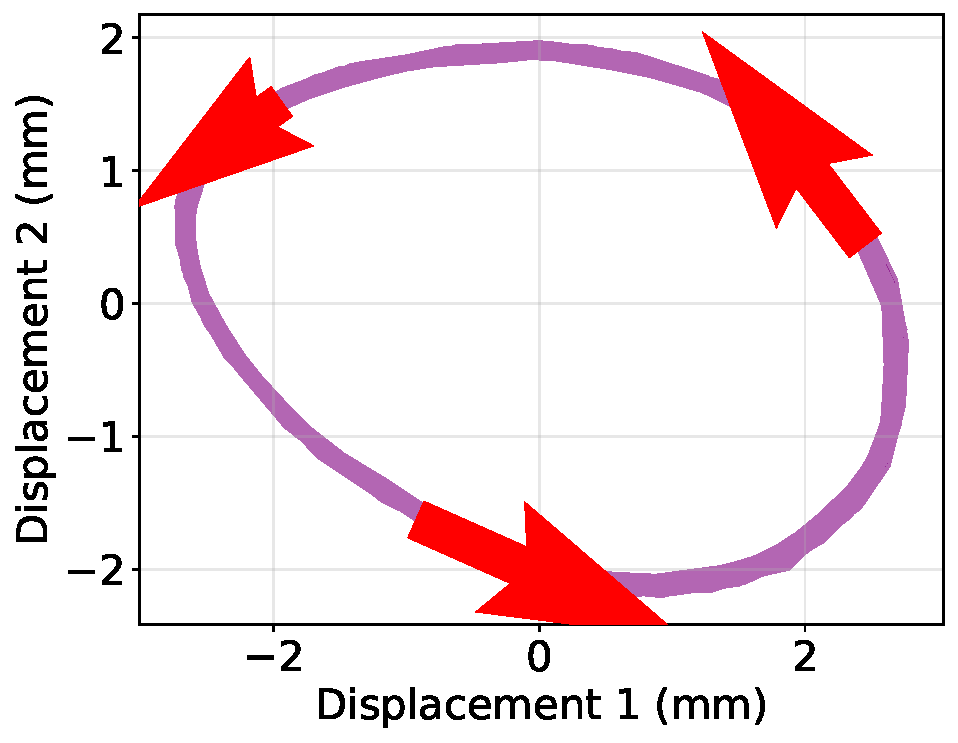
\includegraphics[height=3cm]{limit_cycle_example_2.pdf}
    \caption{}
    \label{fig:exp_limit_cycle}
    \end{center}
\end{subfigure}
\caption{\textbf{Dynamics of one unit.} 
\textbf{\ref{fig:hopf_bif}} Regimes of the dynamics separated by a supercritical Hopf bifurcation. 
\textbf{\ref{fig:hopf_bif}1.} Overdamped regime: $|k_a|<\gamma \sqrt{k_0}$, oscillations die.
\ref{fig:hopf_bif}2. Oscillations regime: $|k_a|>\gamma \sqrt{k_0}$, stable limit cycles with chirality:
 positive ($k_a>0$ counterclockwise) or negative ($k_a<0$ clockwise). 
\textbf{\ref{fig:exp_limit_cycle}} Experimental data in state space displaying the limit cycle. }
\label{fig:diagram_hopf}
\end{figure}

    By plotting the trajectory of the system in state space, i.e. in the $x$-$y$ plane, we can see the effect of the non-reciprocal coupling.
    The system traces out limit cycles above the Hopf bifurcation. Limit cycles are isolated closed trajectories. 
    The fact that they are closed means that they are periodic solutions. They are usually defined in phase space, 
    and they are best visualized when the phase space is two-dimensional. However, our system 
    of equations \eqref{eq_1osc_x} and \eqref{eq_1osc_y} has actually four degrees of freedom: 
    the displacements $x$ and $y$, and their velocities $\xd$ and $\yd$. The phase space is thus four-dimensional.
    However, we can project the trajectories onto the $x$-$y$ plane, and we will see that they also trace out limit cycles there.
    Systems with negative chirality trace out limit cycles in clockwise direction, in which the oscillations of 
    spring $x$ go behind in phase with respect to those of spring $y$.
    Meanwhile systems with positive chirality trace out limit cycles in counterclockwise direction,
    making spring $x$ go ahead in phase with respect to spring $y$. 
    This system's limit cycles are vey specific. From the eigenvector formulas \eqref{eq_1osc_v1} and \eqref{eq_1osc_v2}, 
    we can observe that the two linear actuators differ in value by a constant factor $\pm i = e^{\pm i\pi/2}$. 
    It means that the two actuators have a phase difference of $\pm \pi/2$, and they are said to be in quadrature. 

    % If the actuators have the same amplitude, the limit cycles in this particular case are circles. If the actuators 
    % have the same amplitude but other phase difference, they will trace out ellipses.
    % [precise? Yuan said they are ellipses because the potential is not spherically symetric]

    In conclusion, we use odd elasticity (or non-reciprocity in general) between two linear actuators to achieve stable limit cycles 
    that can oscillate either in clockwise or counterclockwise direction, and they can be used to replace the spin. We refer to the 
    mechanical analogue of spin as oscillator chirality or mechanical spin. 

\subsection{Hopf bifurcation}
\label{subsec:1unit_hopf}

Consider two actuators with the following interactions, which we consider to be the 
most important forces acting on the system: 
linear stiffness, friction, odd elasticity and cubic stiffness. The classical equations of motion are 
\eqref{eq_1osc_x} and \eqref{eq_1osc_y}.
% [use the equations above maybe?] 
% \begin{align}
% \ddot{x}_1 + k_0 x_1 - \gamma \dot{x}_1 - k_c x_1^3 + k_a x_2 &= 0 \\
% \ddot{x}_2 - k_0 x_2 - \gamma \dot{x}_2 - k_c x_2^3 - k_a x_1 &= 0
% \end{align}
We can study the linearized system at the origin. The Jacobian at that point is 
\begin{equation}
    J(0,0,0,0) = \begin{pmatrix}
0 & 0 & 1 & 0 \\
0 & 0 & 0 & 1 \\
-k_0 & k_a & -\gamma & 0 \\
-k_a & -k_0 & 0 & -\gamma
\end{pmatrix}
\end{equation}
and the eigenvalues are 
\begin{equation}
    \lambda = \frac{1}{2}\left(-\gamma \pm \sqrt{\pm 4ik_a - 4k_0 + \gamma^2}\right)
\end{equation}
If we substitute the critical value $k_a^c = \gamma \sqrt{k_0}$, then one can complete the square inside the square root, 
and two of the eigenvalues become purely imaginary: $\lambda = \pm i \sqrt{k_0}$. The fact that two complex conjugate eigenvalues
have vanishing real part is the defining property of a Hopf bifurcation.  
To study the details of the bifurcation, we can perform a change of variables that reduces the order of the ODEs:
\begin{align}
    x(t) &= A(t)e^{i\omega_1 t} + A^*(t)e^{-i\omega_1 t} = z + z* \\
    \xd(t) &= i\omega_1 (A(t)e^{i\omega_1 t} - A^*(t)e^{-i\omega_1 t}) = i\omega_1 (z - z^*) \\
    z &= x - \frac{i}{\omega_1}\xd
\end{align}
The new variable $z$ depends on the position and velocity of the actuator. 
We carry out the same change of variables for $y$, and we denote the new variable by $f$. 
Substituting in the equations of motion, we find that the equations in the new variables are 
\begin{align}
    \zd &= (-\gamma + i\omega_1)z - \left(\alpha + \frac{3ik_c}{\w_1}\right)|z|^2z - \frac{ik_a}{\w_1}f ,\\ %+ \alpha f^2 z^* -2 \alpha |f|^2 z \\
    \dot{f} &= (-\gamma + i\omega_1)f - \left(\alpha + \frac{3ik_c}{\w_2}\right)|f|^2f + \frac{ik_a}{\w_2}z .
\end{align}
These are Stuart-Landau equations \cite{Landau:1944ibh,Stuart_1958,Stuart_1960}. 
It is also the normal form of a Hopf bifurcation. One can obtain the usual normal form 
in polar coordinates by substituting $z=Re^{i\Th}$. One finds
\begin{align}
    \dot{R}_1 &= -\gamma R_1 + \frac{k_a}{\omega_1}R_2 \sin{\Delta\phi}, \\ %- \alpha R_1^3 
    \dot{R}_2 &= -\gamma R_2 + \frac{k_a}{\omega_2}R_1 \sin{\Delta\phi}, \\
    \dot{\phi_1} &= \omega_1 - \frac{3k_c}{\omega_1} R_1^2 -\frac{k_a}{\omega_1}\frac{R_2}{R_1}\cos{(\phi_2-\phi_1)}, \\
    \dot{\phi_2} &= \omega_2 - \frac{3k_c}{\omega_2} R_2^2 +\frac{k_a}{\omega_2}\frac{R_1}{R_2}\cos{(\phi_2-\phi_1)}, \\
    \dot{\Delta\phi} &= \omega_2 - \omega_1 - 3k_c\left(\frac{R_2^2}{\omega_2} - \frac{R_1^2}{\omega_1}\right) 
    + k_a\cos{\Delta\phi} \left(\frac{R_1}{R_2\omega_2} + \frac{R_2}{R_1\omega_1}\right).
\end{align}
Looking at the radial equations, the activity $k_a$ is the responsible for the instability at the origin, while the friction 
$\gamma$ stabilizes the same point. It is the same type of equations as the normal form of a supercritical Hopf bifurcation.
The difference with the archetypical equations is that here the instability is driven by odd elasticity instead of negative damping. 

% This is wrong
% To get the Hopf bifurcation, I must also add the term $\alpha (x^2 + y^2)\xd$. Maybe adding $\alpha x^2 \xd$ is more physical, 
% because the dissipation deppends only one the own oscillator, not on the other one. This also simplifies the equations. 
% Note the last term in $\Delta\phi$ equation is not invariant under sign change, which makes sense. Odd elasticity forces 
% a specific phase difference between actuators. 

% \begin{equation}
% \dot{A} = (\mu - i \Delta)A - (\gamma - i\lambda)|A|^2 A 
% \end{equation}
% $d=\mu-\mu_c, \beta, \gamma, \mu$ are real parameters with approximation $\approx 1$.

% Let $A = R e^{i\varphi} \implies \dot{A} = \dot{R}e^{i\varphi} + i R \dot{\varphi}e^{i\varphi}$

% Real part: $\dot{R} = \mu$

% i.e., let $d \to 0 \implies \dot{A} \to 0$

% \begin{equation}
% (\mu - i\Delta)A = (\gamma - i\alpha)|A|^2 A
% \end{equation}

% If $\mu = \delta |A|^2 \implies |A|^2 = \frac{\mu}{\delta}$

% $-\Delta = \alpha |A|^2 \implies |A|^2 = -\frac{\Delta}{\alpha}$


We can calculate the critical value of activity at the Hopf bifurcation by using a plane wave ansatz.
We start by defining a different complex variable $z = x_1 + i x_2$. 
Close to the Hopf bifurcation, we can neglect the nonlinear terms and the equations of motion reduce to 
one complex second order ODE:
\begin{equation}
\ddot{z} + k_0 z + \gamma \dot{z}  - i k_a z = 0.  %+ k_c |z|^2 z neglected
\end{equation}
It is essentially a competition between damping $\gamma$ and active coupling $k_a$.
Assume a solution of the form $z = e^{\lambda t}$:
\begin{equation}
\lambda^2 + \gamma\lambda + k_0 - i k_a = 0.
\end{equation}
A Hopf bifurcation happens precisely when $\text{Re}(\lambda) = 0$ and $ \text{Im}(\lambda) \neq 0$,
we can substitute $\lambda = i\omega_c$ into the characteristic equation:
\begin{equation}
-\omega_c^2 + i \gamma \omega_c + k_0 - i k_a = 0.
\end{equation}
Solving for the real and imaginary parts independently
\begin{align}
\text{Real part:} \quad & -\omega_c^2 + k_0 = 0 \implies \omega_c = \sqrt{k_0}, \\
\text{Imaginary part:} \quad & \gamma \omega_c - k_a = 0 \implies \omega_c = \frac{k_a}{\gamma},
\end{align}
we find again the critical coupling threshold $k_a^c$:
\begin{equation}
k_a^c = \gamma \sqrt{k_0}.
\end{equation}

To know the behaviour of the limit cycle close to the bifurcation, we perform stability analysis. 
We substitute $z = R e^{i\omega t}$ for radius/phase separation, and by setting $\dot{R} = 0$ we find:
\begin{equation}
-\omega^2 R + k_0 R + i \omega \gamma R + k_c R^3 - i k_a R = 0.
\end{equation}
We can separate again into real and imaginary parts:
\begin{align}
\text{Real part:} \quad & -\omega^2 + k_0 - k_c R^2 = 0 \implies \omega^2 = k_0 + k_c R^2, \\
\text{Imaginary part:} \quad & \omega \gamma = k_a \implies \omega = \frac{k_a}{\gamma}.
\end{align}
The imaginary equation indicates that the frequency of the limit cycle scales linearly with the activity.
Combining both parts allows solving for the radius $R^2$:
\begin{align}
\frac{k_a^2}{\gamma^2} &= k_0 + k_c R^2 \\
R^2 &= \frac{1}{k_c} \left( \frac{k_a^2}{\gamma^2} - k_0 \right) ,\\
R^2 &= \frac{1}{k_c \gamma^2} \left( k_a^2 - \gamma^2 k_0 \right) .
\end{align}
We use the previous result $(k_a^c)^2 = \gamma^2 k_0$ to simplify
\begin{equation}
R^2 = \frac{1}{k_c \gamma^2} \left( k_a^2 - (k_a^c)^2 \right) = \frac{1}{k_c \gamma^2} (k_a - k_a^c)(k_a + k_a^c),
\end{equation}
and approximating near the threshold where $k_a + k_a^c \approx 2k_a^c$, we obtain
\begin{equation}
R \approx \sqrt{\frac{2 k_a^c}{k_c \gamma^2} (k_a - k_a^c)}.
\end{equation}
This confirms the square-root behavior for the limit cycle radius above the threshold, 
together with the linear behaviour of the frequency. 

Far from the Hopf bifurcation, one needs to include higher order terms $A^5, A^7$... that give exponents $1/4, 1/6$... 
to the activity for the function of the radius. These higher order terms make the slope flatter until it is constant. 

The limit cycles we discussed occur in the 4-dimensional phase space $(x_1, \xd_1, x_2, \xd_2)$. Nevertheless, we can project the trajectory 
to the 2-dimensional state space $(x_1, x_2)$. As the phase difference between the two springs is enforced to be $\Delta\phi=\frac{\pi}{2}$ 
by the odd elastic interactions, the trajectory in the lower-dimensional space is an ellipse. 

\subsection{Experiments}
\label{sec:one_node_exp}
%[move to section 2 experimental setup?]

\begin{figure}[htbp]
  \centering
  \begin{subfigure}[b]{0.48\textwidth}
    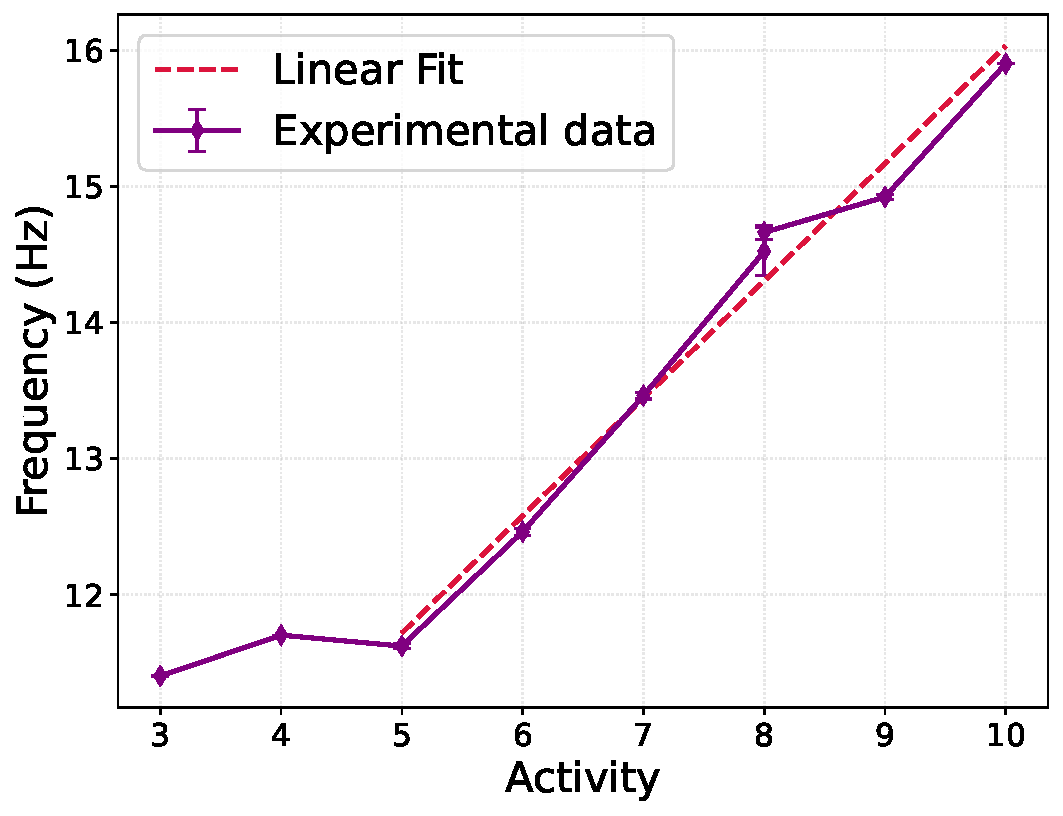
\includegraphics[width=\textwidth]{linear_frequency_scaling_one_node_2.pdf}
    \caption{}
    \label{fig:1unit_freq_scaling}
  \end{subfigure}
  \hfill
  \begin{subfigure}[b]{0.48\textwidth}
    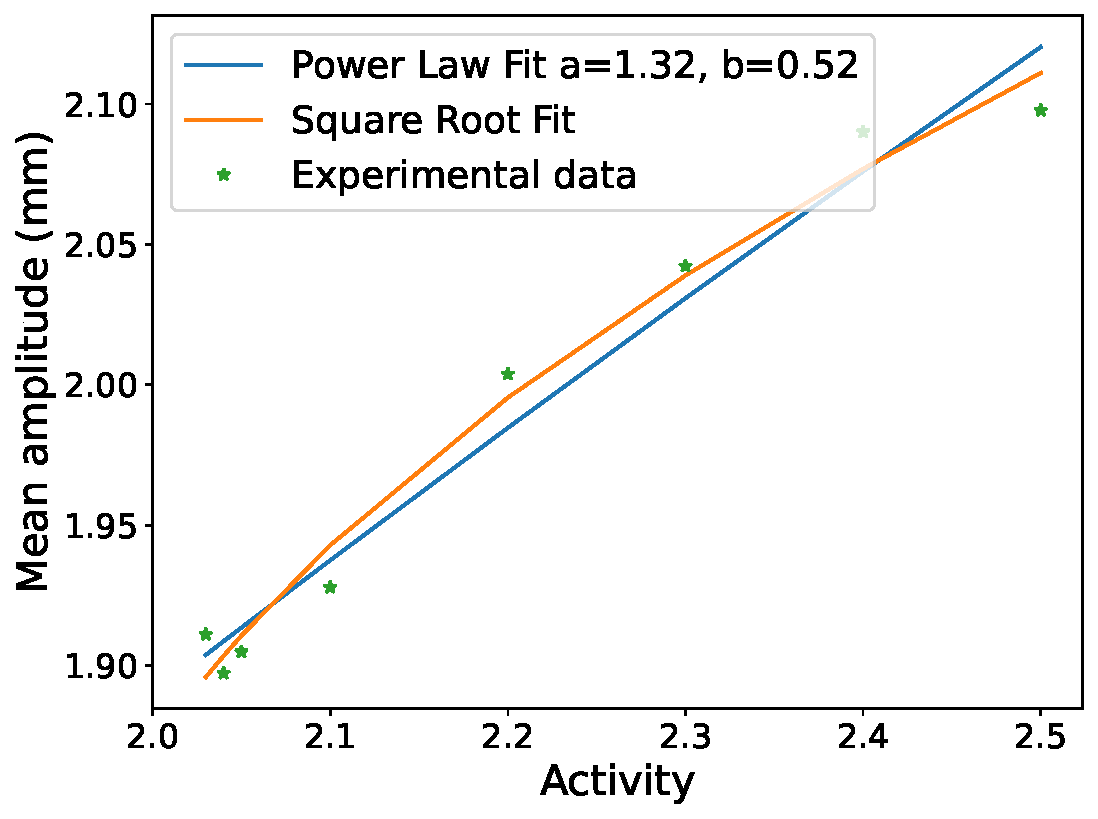
\includegraphics[width=\textwidth]{amplitude_scaling_Hopf_2.pdf}
    \caption{}
    \label{fig:1unit_amp_scaling}
  \end{subfigure}
  \caption{\textbf{Limit cycle scalings close to Hopf bifurcation.} 
  \textbf{\ref{fig:1unit_freq_scaling}} Linear scaling of frequency with activity parameter. 
  \textbf{\ref{fig:1unit_freq_scaling}} Square root scaling of amplitude with activity parameter. 
  The experimental results agree with the theoretical predictions of the supercritical Hopf bifurcation. }
\end{figure}

The regime below the Hopf bifurcation, where the system goes to rest, is not interesting, so we focus on the regime 
    above the Hopf bifurcation where the system traces out limit cycles. 
    There is only one parameter to control in the experiments, and that is the activity $k_a$. 
    The rest of coupling coefficients in equations \eqref{eq_1osc_x} and \eqref{eq_1osc_y} are 
    determined by the actuators' mechanical properties, which we don't change. We can decompose the analysis of the limit cycles into two: 
    the phase and the amplitude.
    %[does this belong here?] 


We observe that the frequency of the limit cycle increases when we increase the gain, 
see figure \ref{one_node_exp_results}. Moreover, the frequency increases linearly, as predicted by 
the supercritical Hopf bifurcation. The measurements of the amplitude of oscillation have great variability. 
Both actuators forming the unit oscillate with the same frequency, because they are coupled non-reciprocally.
But they don't oscillate with quite the same amplitude, and this is due to small differences in each of the actuators. 
Keep in mind that the actuators are several years old because they were made for another setup. Some of them were crooked or 
broken and had to be repaired, and that led to the system being considerably inhomogeneus. 
For that reason, we also measured the motion of another unit. The amplitude and frequency of the limit cycle are shown in 
figure \ref{one_node_exp_results_2}. Again, we see that the frequency increases linearly with activity. At lower values 
of activity, the slope of the frequency flattens. The amplitude stays roughly the same for a big range of activities. 
This observation might be a consequence of the actuators having a hard stop at their ends. Above a certain value of activity, 
the actuator reaches its maximum displacements. Increasing the activity beyond doesn't make the amplitude grow further, 
but it does make the oscillations go faster. 

\begin{figure}
    \begin{subfigure}[b]{0.48\textwidth}
    \begin{center}
        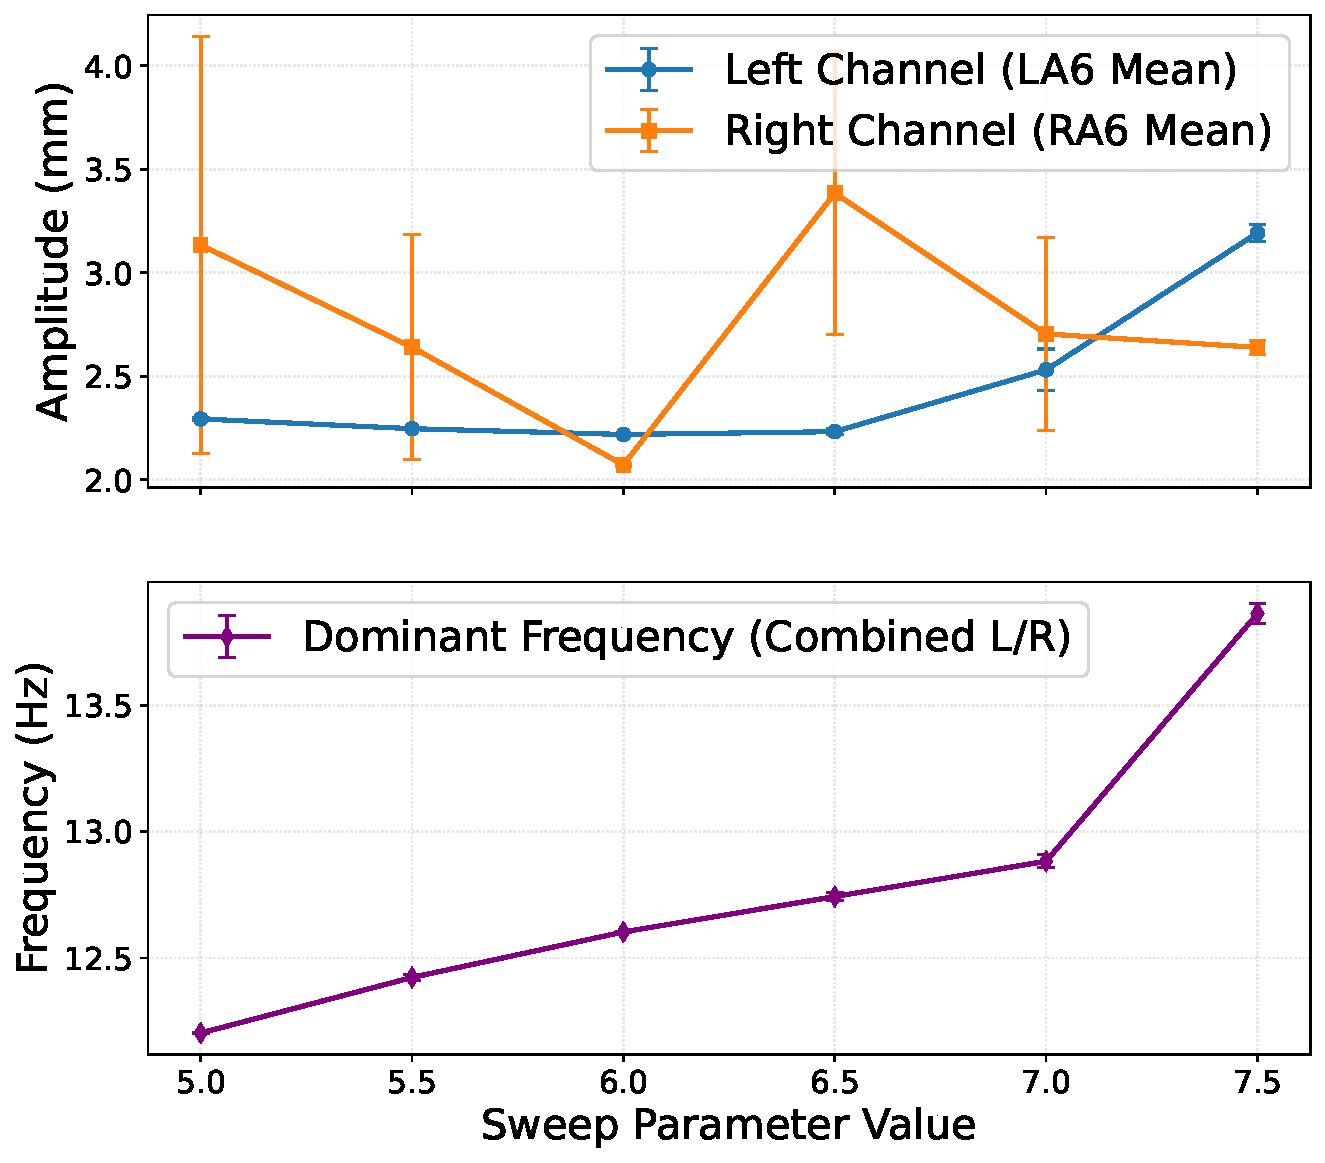
\includegraphics[width=\textwidth]{one_unit_results_a6.pdf}
        \caption{}
        \label{one_node_exp_results}
    \end{center}
\end{subfigure}
\begin{subfigure}[b]{0.48\textwidth}
        \begin{center}
        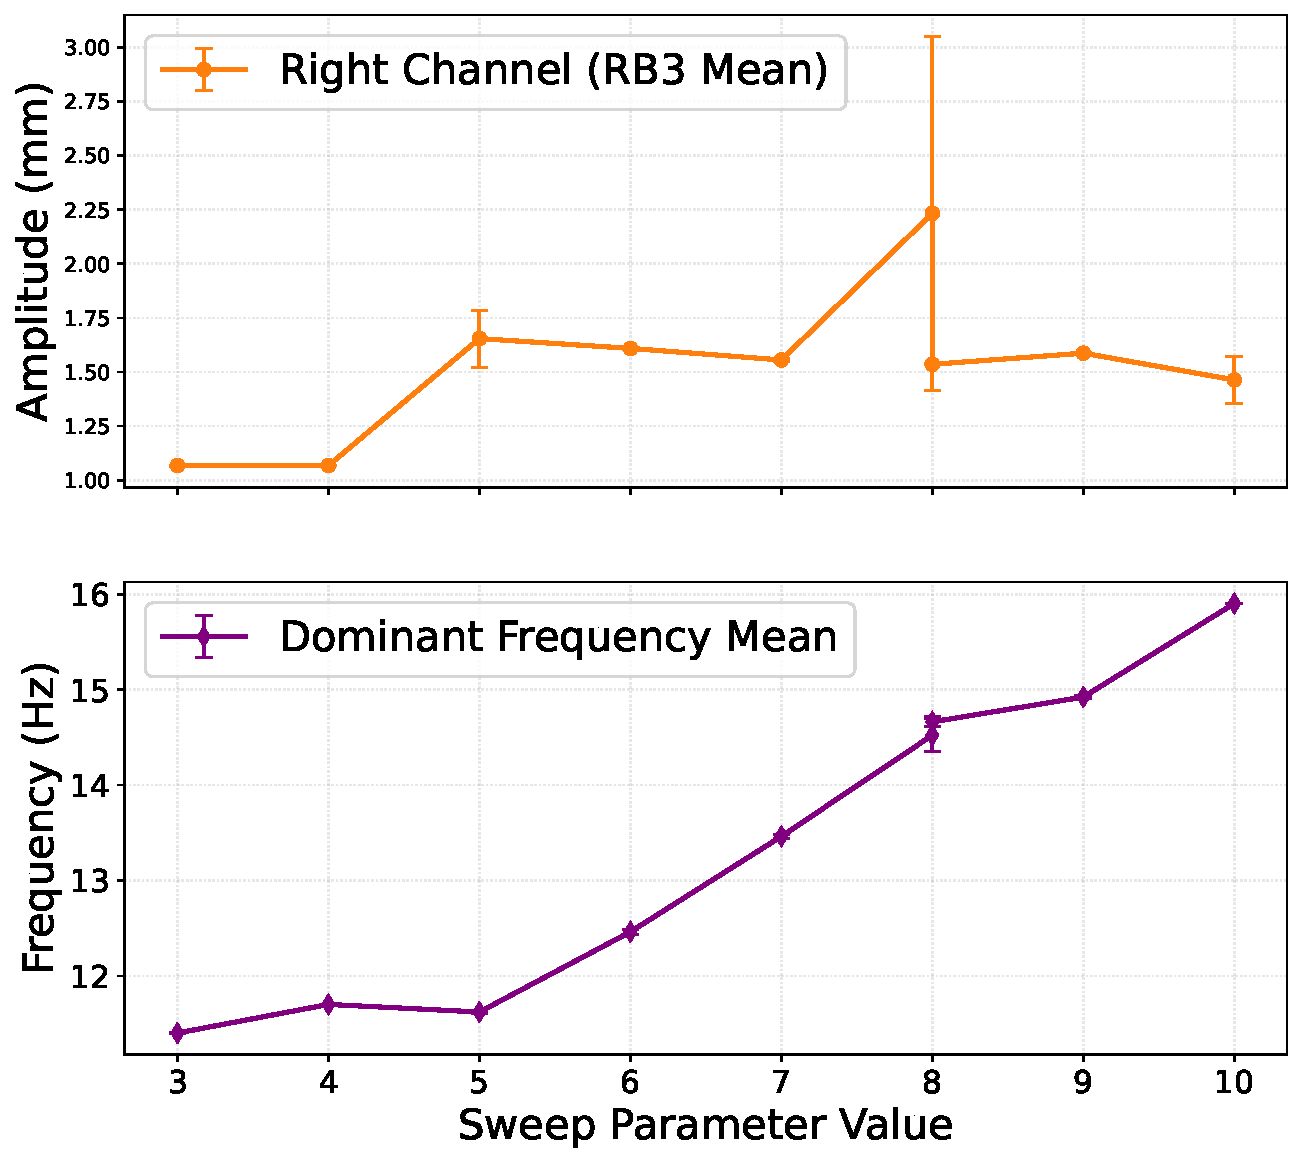
\includegraphics[width=\textwidth]{one_unit_results_b3.pdf}
        \caption{}
        \label{one_node_exp_results_2}
    \end{center}
\end{subfigure}
\caption{\textbf{Experimental data of single unit limit cycles. }
Characteristics of the limit cycles, amplitude and frequency, for separate single units. 
Top: amplitude of limit cycle. Bottom: natural frequency. The x-axis is the activity parameter of odd elasticity 
of the unit. 
\textbf{\ref{one_node_exp_results}} First unit. The frequency increases linearly with activity. The amplitude of the 
left actuator (blue) stays constant at first and the increases. The amplitude of the right actuator (orange) has large error bars, 
demonstrating its variability. 
\textbf{\ref{one_node_exp_results_2}} Second unit. The frequency increases linearly with activity. The amplitude is 
the same for the first two activity values. For higher activity, the amplitude is larger, but it remains constant throughout.  
}
\end{figure}

% We also wondered what happened close to the Hopf bifurcation. Figure \ref{fig:one_node_Hopf} shows measurements 
% done right after the onset of limit cycles. In fact, for $k_a = 2.0$, the oscillations died out and there was no limit cycle. 
% Figure \ref{subfig:plot_a} shows how the oscillation amplitude increases with the activity. The fitted curves suggest a power law 
% with exponent around 0.8. The scaling derived from the theory is a square root. 
% [why the difference]
% The other figure \ref{subfig:plot_b} shows the frequencies measured as a function of the gain. The surprising things is that 
% the frequencies seem to be quantized. However, this is easily explained by what we said earlier. The precision in 
% frequency measurements is determined by the time of recording. In this set of measurements, $T=\SI{5}{s}$ and so the 
% precision is $\varDelta f = \frac{1}{5s}= \SI{0.2}{Hz}$. That explains the height of each step. Thus, measuring the frequency close 
% to the Hopf bifurcation is conditioned by the precision. Nevertheless, we already verified the linear scaling in frequency from the Hopf 
% bifurcation in figures \ref{one_node_exp_results} and \ref{one_node_exp_results_2}.

% \begin{figure}[htbp]
%     \centering
%     % === SUBPLOT A ===
%     \begin{subfigure}[b]{0.48\textwidth}
%         \centering
%         % Replace 'example-image-a' with your plot's filename (e.g., 'plot_T0.pdf')
%         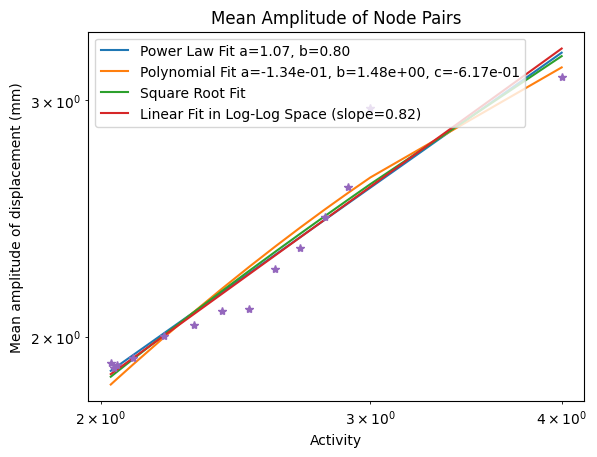
\includegraphics[width=\textwidth]{one_node_amplitude_fit.png}
%         \caption{fig}
%         \label{subfig:plot_a}
%     \end{subfigure}
%     \hfill % Adds horizontal space to push the subplots to the margins
%     % === SUBPLOT B ===
%     \begin{subfigure}[b]{0.48\textwidth}
%         \centering
%         % Replace 'example-image-b' with your plot's filename (e.g., 'plot_B0.pdf')
%         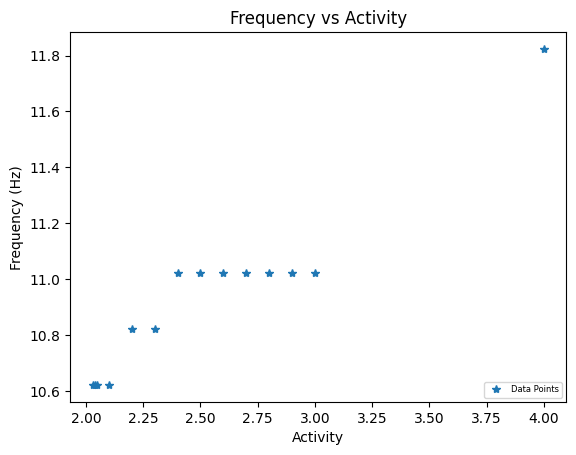
\includegraphics[width=\textwidth]{on_node_Hopf_freq_vs_act.png}
%         \caption{fig}
%         \label{subfig:plot_b}
%     \end{subfigure}
    
%     % Global caption and label for the entire figure layout
%     \caption{fig}
%     \label{fig:one_node_Hopf}
% \end{figure}

% [can lso include freq vs amp fit that gives alpha non-isochronous paremeter]
% From the theory, we know that the nonlinearities have an effect on the frequency of oscillation. 
% To a first approximation, $\dot{\Th} \sim \omega - \alpha R^2$, where $\alpha$ is the non-isochrounous parameter and 
% $R$ is the amplitude of oscillation. If we plot the amplitude on the x-axis and the oscillation frequency on the y-axis, we can
% fit the data to obtain the non-isochronous parameter. The results show $\alpha$ is negative.  

% \begin{figure}
%     \begin{center}
%         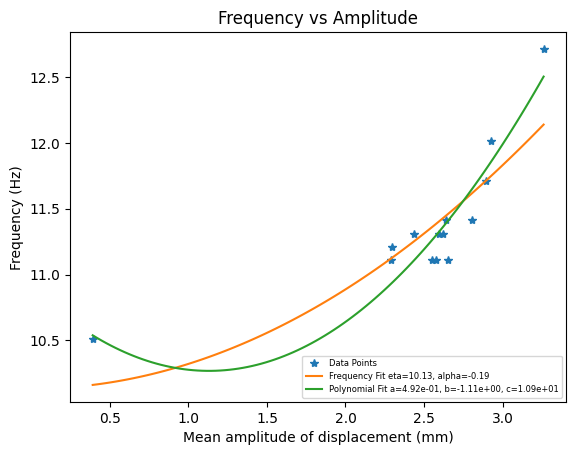
\includegraphics[width = 0.5\textwidth]{one_node_alpha_fit.png}
%         \caption{Figure}
%         \label{alpha_fit}
%     \end{center}
% \end{figure}

\section{Two non-reciprocal units}
\label{sec:two_units}
In this section we couple two non-reciprocal units with an elastic band. 

\subsection{Theory}
\label{subsec:2units_theory}

In this section we analyse the classical dynamical equations of 2 non-reciprocal units coupled together via an elastic band. 
Each unit contains 2 actuators. We use the method of multiple scales to find the complex amplitude equations describing the slow dynamics of the system. 
Next we switch variables to real amplitude and phase. Finally, we interpret the results in terms of synchronization between the two oscillators.

%% need to add diagram of the system with tikz
% [add explanation of which actuator is which]
\begin{figure}[hbtp]
\begin{center}
    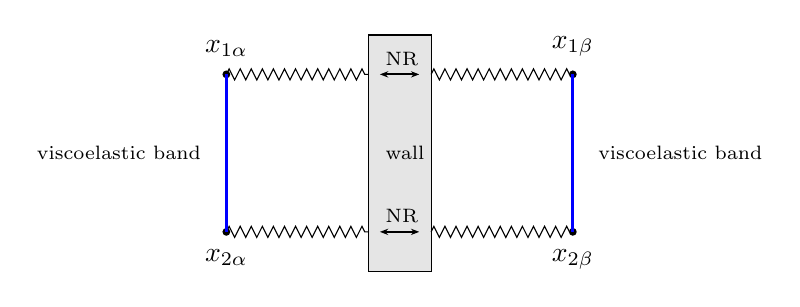
\begin{tikzpicture}[scale=1,
    spring/.style={decorate,decoration={zigzag,segment length=4,amplitude=2}},
    active/.style={circle,fill=black,inner sep=1pt}
]

% Vertical slab
\draw[fill=gray!20] (0,-1.5) rectangle (0.8,1.5);

% Odd elasticity arrows inside slab
\draw[<->,thick] (0.15,1) -- (0.65,1);
\draw[<->,thick] (0.15,-1) -- (0.65,-1);
\node[font=\scriptsize,anchor=west] at (0.1,1.2) {NR};
\node[font=\scriptsize,anchor=west] at (0.1,-0.8) {NR};
\node[font=\scriptsize,anchor=west] at (0.1,0) {wall};

% arrows dis

% Top left spring + active actuator
\draw[spring] (-1.8,1) -- (0,1);        % spring
\node[active] at (-1.8,1) {};           % active symbol
\node[anchor=south] at (-1.8,1.1) {$x_{1\alpha}$};

% Bottom left spring + active actuator
\draw[spring] (-1.8,-1) -- (0,-1);
\node[active] at (-1.8,-1) {};
\node[anchor=north] at (-1.8,-1.1) {$x_{2\alpha}$};

% Top right spring + active actuator
\draw[spring] (0.8,1) -- (2.6,1);
\node[active] at (2.6,1) {};
\node[anchor=south] at (2.6,1.1) {$x_{1\beta}$};

% Bottom right spring + active actuator
\draw[spring] (0.8,-1) -- (2.6,-1);
\node[active] at (2.6,-1) {};
\node[anchor=north] at (2.6,-1.1) {$x_{2\beta}$};

% Vertical elastic bands on each side (connecting springs on same side)
\draw[very thick,blue] (-1.8,1) -- (-1.8,-1);
\draw[very thick,blue] (2.6,1) -- (2.6,-1);

% Band labels (one is enough, but you can keep both if you like)
\node[font=\scriptsize,anchor=east] at (-2.0,0) {viscoelastic band};
\node[font=\scriptsize,anchor=west] at (2.8,0) {viscoelastic band};

\end{tikzpicture}
\end{center}
\caption{\textbf{Schematic representation of two coupled non-reciprocal units.}
The actuators are fixed to the wall structure. 
The actuators on the same side of the wall interact through the viscoelastic band, while
the mirror actuators to each side of the wall are coupled non-reciprocally (NR).
The displacement of the actuators is perpendicular to the wall. }
\label{fig:diagram_2units}
\end{figure}

Since there are 2 actuators per non-reciprocal unit, we have 4 actuators and 8 degrees of freedom in total. 
We denote the displacements of the actuators in unit 1 as $x_{1\alpha}$ and $x_{1\beta}$, and in unit 2 as $x_{2\alpha}$ and $x_{2\beta}$, 
as shown in figure \ref{fig:diagram_2units}. 
The actuators are classical, so we can use Newton's second law to write down the equations of motion:
\begin{equation}
\begin{aligned}
\ddot{x}_{1\alpha} + \omega x_{1\alpha} &= 
\epsilon(\omega - \omega_{1\alpha}^2) x_{1\alpha}
-\epsilon \gamma_{1\alpha} \dot{x}_{1\alpha}
- \epsilon k_{c,1\alpha} x_{1\alpha}^3
+ \epsilon k_a^{1} x_{1\beta} 
+ \epsilon k_v (\dot{x}_{2\alpha} - \dot{x}_{1\alpha})
+ \frac{\epsilon k_b}{2 L^2} (x_{2\alpha} - x_{1\alpha})^3, \\
\ddot{x}_{1\beta} + \omega x_{1\beta} &= 
\epsilon(\omega - \omega_{1\beta}^2) x_{1\beta}
-\epsilon \gamma_{1\beta} \dot{x}_{1\beta}
- \epsilon k_{c,1\beta} x_{1\beta}^3
- \epsilon k_a^{1} x_{1\alpha}
+ \epsilon k_v (\dot{x}_{2\beta} - \dot{x}_{1\beta})
+ \frac{\epsilon k_b}{2 L^2} (x_{2\beta} - x_{1\beta})^3, \\
\ddot{x}_{2\alpha} + \omega x_{2\alpha} &= 
\epsilon(\omega - \omega_{2\alpha}^2) x_{2\alpha}
-\epsilon \gamma_{2\alpha} \dot{x}_{2\alpha}
- \epsilon k_{c,2\alpha} x_{2\alpha}^3
+ \epsilon k_a^{2} x_{2\beta} 
+ \epsilon k_v (\dot{x}_{1\alpha} - \dot{x}_{2\alpha})
+ \frac{\epsilon k_b}{2 L^2} (x_{1\alpha} - x_{2\alpha})^3, \\
\ddot{x}_{2\beta} + \omega x_{2\beta} &= 
\epsilon(\omega - \omega_{2\beta}^2) x_{2\beta}
-\epsilon \gamma_{2\beta} \dot{x}_{2\beta}
- \epsilon k_{c,2\beta} x_{2\beta}^3
- \epsilon k_a^{2} x_{2\alpha}
+ \epsilon k_v (\dot{x}_{1\beta} - \dot{x}_{2\beta})
+ \frac{\epsilon k_b}{2 L^2} (x_{1\beta} - x_{2\beta})^3,
\end{aligned}
\label{eq:mse_eom_2units}
\end{equation}
where $\omega_{u\sigma}$ is the natural frequency of actuator $\sigma\in\{\alpha,\beta\}$ in unit $u\in\{1,2\}$, 
$\gamma_{u\sigma}$ is the damping coefficient, $k_{c,u\sigma}$ is the nonlinear saturation stiffness, 
$k_a^{u}$ is the non-reciprocal coupling within unit $u$, 
$k_v$ is the viscous coupling of the elastic band, $k_b$ is the coupling strength of the elastic band, and $L$ 
is the distance between the actuators at rest. The parameter $\epsilon$ indicates that all the perturbations, 
detuning, damping, nonlinear stiffness, non-reciprocal coupling and neighbour coupling, are weak compared to the harmonic oscillator terms.

After performing the theoretical derivation described in section \ref{subsec:theoretical_procedure}, one ends up with 
differential equations for the amplitude and phase of each of the actuators. For the details of the derivation, 
see section \ref{subsec:2units_mse_derivation}. The resulting equation for the radius/amplitude of the actuator $x_{1\alpha}$ is
\begin{equation}
\begin{aligned}
\dot{R}_{1\alpha} &= -\frac{1}{2} \gamma_{1\alpha} R_{1\alpha} 
+ \frac{3k_a^{1}}{2\omega} R_{1\beta} \sin(\phi_{1\beta} - \phi_{1\alpha}) 
+ \frac{k_v}{2} \big(R_{2\alpha}\sin{(\phi_{2\alpha} - \phi_{1\alpha})} - R_{1\alpha}\big) \\
&\quad + \frac{3k_b}{4\omega L^2} \sin(\phi_{2\alpha} - \phi_{1\alpha}) 
\left( R_{2\alpha}^3 + R_{1\alpha}^2 R_{2\alpha} - 2R_{2\alpha}^2 R_{1\alpha} \cos(\phi_{2\alpha} - \phi_{1\alpha}) \right),
\label{eq_MSE_2nodes_amplitude}
\end{aligned}
\end{equation}
and the equation for the phase is
\begin{equation}
\begin{aligned}
\dot{\phi}_{1\alpha} &= \omega_{1\alpha} + \frac{3k_{c,1\alpha}}{2\omega} R_{1\alpha}^2 
- \frac{3k_a^{1}}{2\omega} \frac{R_{1\beta}}{R_{1\alpha}} \cos(\phi_{1\beta} - \phi_{1\alpha}) 
+ \frac{k_v}{2} \left(\frac{R_{2\alpha}}{R_{1\alpha}}\sin{(\phi_{2\alpha} - \phi_{1\alpha})} - 1\right) \\
&\quad - \frac{3k_b}{4\omega L^2} \left[ \cos(\phi_{2\alpha} - \phi_{1\alpha}) 
\left( \frac{R_{2\alpha}^3}{R_{1\alpha}} + R_{1\alpha} R_{2\alpha} - 2R_{2\alpha}^2 \cos(\phi_{2\alpha} - \phi_{1\alpha}) \right) \right. \\
&\quad \left. - R_{2\alpha}^2 - R_{1\alpha}^2 + 2R_{2\alpha} R_{1\alpha} \cos(\phi_{2\alpha} - \phi_{1\alpha}) \right].
\label{eq_MSE_2nodes_phase}
\end{aligned}
\end{equation}
These are the equations describing the motion of the first actuator in unit 1. 
The equations for the other actuators ($x_{1\beta}$, $x_{2\alpha}$, $x_{2\beta}$) are obtained in the same way and differ only in some of the indices. 

In the amplitude equation \eqref{eq_MSE_2nodes_amplitude}, there are four terms. The first one is negative, 
so it reduces the amplitude, yielding a stable origin. It is no surprise that it is the effect originating from friction $\gamma_{1\alpha}$. 
The sign of the second term depends on the sign of the activity parameter and on the phase difference between the actuators within the same unit 
($\phi_{1\beta} - \phi_{1\alpha}$). The activity term can overcome the damping term, and lead to a stable nonzero value of the amplitude. 
In other words, it generates the limit cycles. It is most influential when the actuators are in quadrature. This agrees with our discussions in section \ref{sec:1unit}.
The third term comes from the viscous coupling of the elastic band between units 1 and 2 (actuators $1\alpha$ and $2\alpha$). 
The units are synchronized when their phases $\phi_{1\alpha} = \phi_{2\alpha}$ are equal. In that case, the term is negative and stabilizes the origin. 
The fourth term originates from the interactions through the elastic band. If the units are synchronized ($\phi_{2\alpha}=\phi_{1\alpha}$), 
the whole term vanishes. Then, the equation reduces to that of an uncoupled unit. In other words, 
if the units synchronize, then they oscillate with their natural amplitude.  

The phase equation \eqref{eq_MSE_2nodes_phase} resembles a Kuramoto-type of model. 
We can compare the coefficients with experimental data. The first term is the natural frequency of actuator $1\alpha$. 
The second term is a non-isochronous term: the radius of oscillation affects the frequency. 
The third term is a usual Kuramoto coupling between the two actuators within unit 1 ($1\alpha$ and $1\beta$). 
As we mentioned before, odd elasticity breaks reciprocity between the actuators. That is why the term is proportional to 
the cosine instead of the sine of the phase difference. The result is that the actuators within one unit are in quadrature, 
with phase difference $\phi_{1\beta}-\phi_{1\alpha} = \pm \frac{\pi}{2}$, just like what we saw in section \ref{subsec:1unit_theory}. 
The viscous term is another Kuramoto interaction, but now between actuators from different units 
($1\alpha$ and $2\alpha$) that are interacting through the elastic band. An important feature is that it is proportional to the sine of the phase difference.
Therefore, the viscous coupling seems to be the synchronizing term, as we saw in section \ref{subsec:sync}.
Also note that the coupling is proportional to the ratio of radii $\frac{R_{2\alpha}}{R_{1\alpha}}$. 
The last term is a more complicated Kuramoto type of coupling of cosine functions, 
which is a consequence of the cubic elastic neighbour coupling. Since the cosine is even, the elastic coupling term
does not lead to the synchronization of units. This came as a surprise at first. Our primitive model had no viscous interaction 
terms from the band. Therefore, we arrived at a Kuramoto-like phase equation with no synchronizing term. 
We realized that such a synchronizing term needed to be imaginary in the Stuart-Landau equations \eqref{eq_MSE_2nodes_complex_amplitude}.
That meant the interaction depended on the velocity rather than on the position of the actuators. Hence, we added the viscous 
interaction in the equations of motion \eqref{eq:mse_eom_2units}, which indeed was the synchronizing term. 
The reason is that the elastic term is conservative. By Liouville's theorem, the phase space volume remains constant under time evolution. 
If the interaction were not conservative, then the phase space volume would shrink towards an attractor. This is precisely 
the case of the viscous interaction, which dissipates energy. The key idea is that synchronization involves the convergence 
of many different initial states to the same trajectory. In the case of two coupled units, the phase space has eight dimensions,
since there are four actuators and each one has position and velocity. Synchronization converges a region of the phase space to 
evolve into a single curve. In consequence, synchronization reduces the phase space volume. Therefore, the elastic term 
cannot synchronize, but the viscous term can.

We can also consider some simplified limits of equations \eqref{eq_MSE_2nodes_amplitude} and \eqref{eq_MSE_2nodes_phase}. 
Actuators $1\alpha$ and $1\beta$ are coupled non-reciprocally, so their phases relock to $|\phi_{1\beta} - \phi_{1\alpha}| = \pi/2$. 
This means that the non-reciprocal coupling term is maximal in the radius equation, and it is zero in the phase equation.
The same thing happens between actuators $2\alpha$ and $2\beta$. 
We can also consider the synchronization regime, when the limit cycles of units 1 and 2 oscillate with the same frequency. 
In the case of complete synchronization (for the $\alpha$-actuators), both oscillators have the same phase: $\phi_{2\alpha} = \phi_{1\alpha}$. 
In this limit, the neighbour coupling term in the amplitude equation vanishes, and the neighbour coupling term 
in the phase equation simplifies:
\begin{align}
\dot{R}_{1\alpha} &= -\frac{1}{2} \gamma_{1\alpha} R_{1\alpha} + \frac{3k_a^{1}}{2\omega} R_{1\beta} 
+ \frac{k_v}{2}(R_{2\alpha} - R_{1\alpha}),  \label{eq_sync_amplitude_simplified}\\
\dot{\phi}_{1\alpha} &= -(\omega - \omega_{1\alpha}) + \frac{3k_{c,1\alpha}}{2\omega} R_{1\alpha}^2 
- \frac{k_v}{2} + \frac{3k_b}{4\omega L^2} \frac{(R_{2\alpha}-R_{1\alpha})^2}{R_{1\alpha}}.
\end{align}

Note that the synchronization frequency is not the average of the original frequencies. One would get the average of the original 
frequencies if the amplitude played no role in the interaction, and only the phase did. One way to show this is to 
start from a Kuramoto-type of model whose dynamics are: 
\begin{align}
    \dot{\Theta}_1 &= \omega_1 + K_1 \sin(\Theta_2 - \Theta_1), \\
    \dot{\Theta}_2 &= \omega_2 + K_2 \sin(\Theta_1 - \Theta_2).
\end{align}
If we impose the synchronization condition $\dot{\Theta}_1 = \dot{\Theta}_2 := \Omega$, in the case in which the coupling is the same 
$K_1=K_2$, we get that the synchronization frequency is given by
\begin{equation}
    \Omega = \frac{\omega_1 + \omega_2}{2}.
\end{equation}
But in our setup, the amplitude does play a role in the interaction. The larger the amplitude of the first node, 
the stronger the coupling feels for the second node. In mathematical terms, we expect $K_1\propto R_2$ and $K_2 \propto R_1$. 
If we assume that the couplings are different $K_1\neq K_2$ and massage the expression 
$K_2 \dot{\Theta}_1 + K_1 \dot{\Theta}_2 = \Omega(K_1+K_2)$, we get that the synchronization frequency is given by
\begin{equation}
    \Omega = \frac{K_2 \omega_1 + K_1 \omega_2}{K_1 + K_2}.
    \label{eq:freq_diff_coupling}
\end{equation}
The crossed indices in the numerator make sense. If $K_1$ is very large, that means that the influence of oscillator 2 on oscillator 1 
is very strong, and therefore the synchronization frequency is closer to $\omega_2$. On the other hand, 
if $K_2$ is very large, that means that the influence of oscillator 1 on oscillator 2 is very strong, 
and therefore the synchronization frequency is close to $\omega_1$.

In section \ref{subsec:2units_mse_derivation}, we obtained what the couplings $K_i$ were. Besides the constant factors, 
they were proportional to the ratio of the amplitudes: $K_1 = \frac{R_2}{R_1}$. Substituting the couplings in 
equation \eqref{eq:freq_diff_coupling}, we find
\begin{equation}
    \Omega = \frac{R_1^2 \omega_1 + R_2^2 \omega_2}{R_1^2 + R_2^2}.
\end{equation}

%%%%%%%%%%%%%%%%%%%%%%%%%%%%%%%%%%%%%%%%%%%%%%%%%%%%
\begin{figure}[hbtp]
    \begin{subfigure}[b]{\textwidth} 
      \begin{center}
        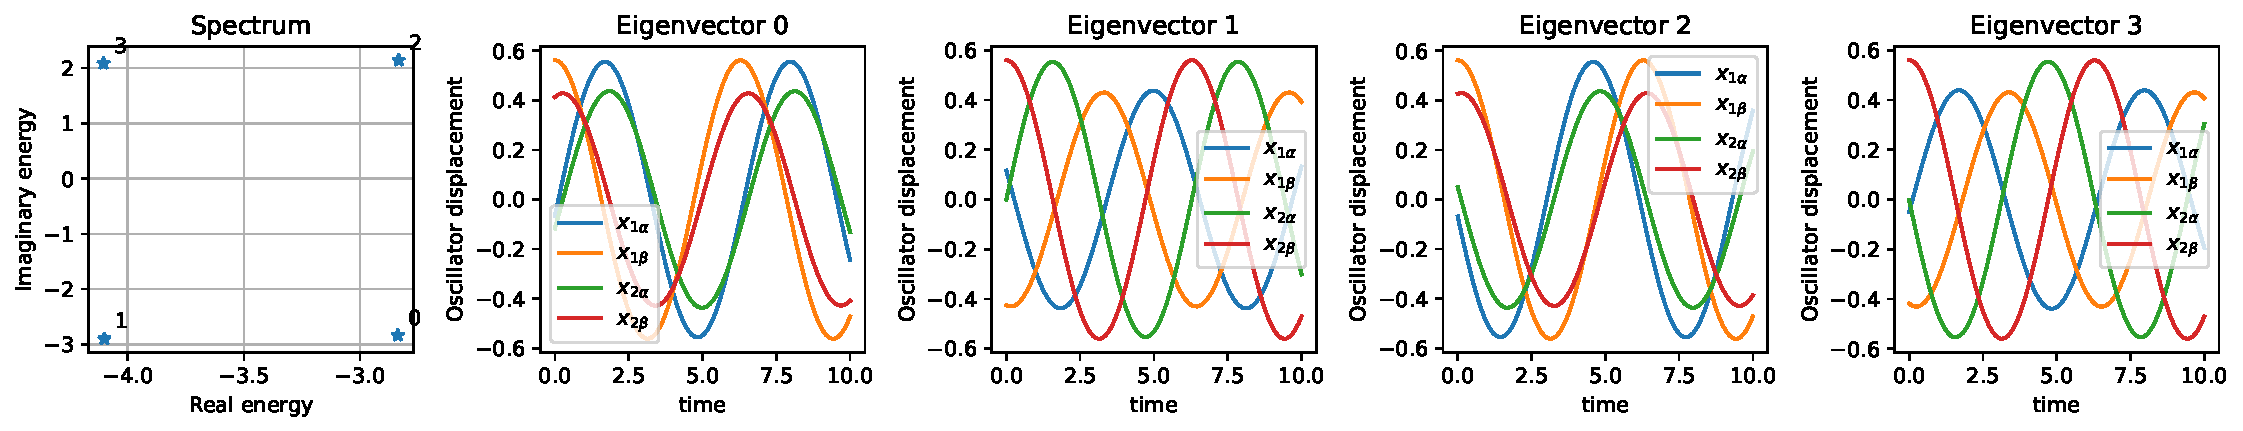
\includegraphics[width=\textwidth]{spectrum_2units_same_chir.pdf}
    \end{center} 
    \caption{}
    \label{subfig:spectrum_2units_same_chir}
    \end{subfigure}
    \begin{subfigure}[b]{\textwidth}
        \begin{center}
        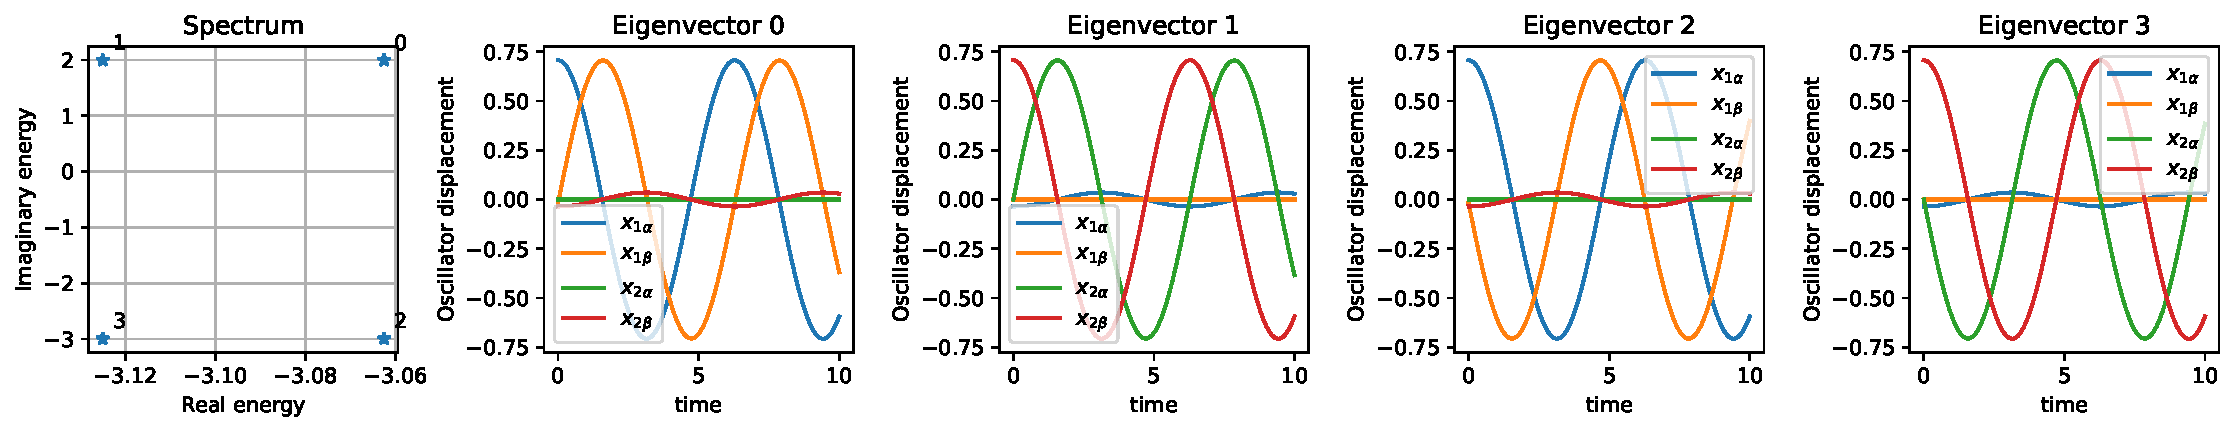
\includegraphics[width=\textwidth]{spectrum_2units_opp_chir.pdf}
    \end{center} 
    \caption{} 
    \label{subfig:spectrum_2units_opp_chir}
    \end{subfigure}
    \begin{subfigure}[b]{\textwidth}
        \begin{center}
        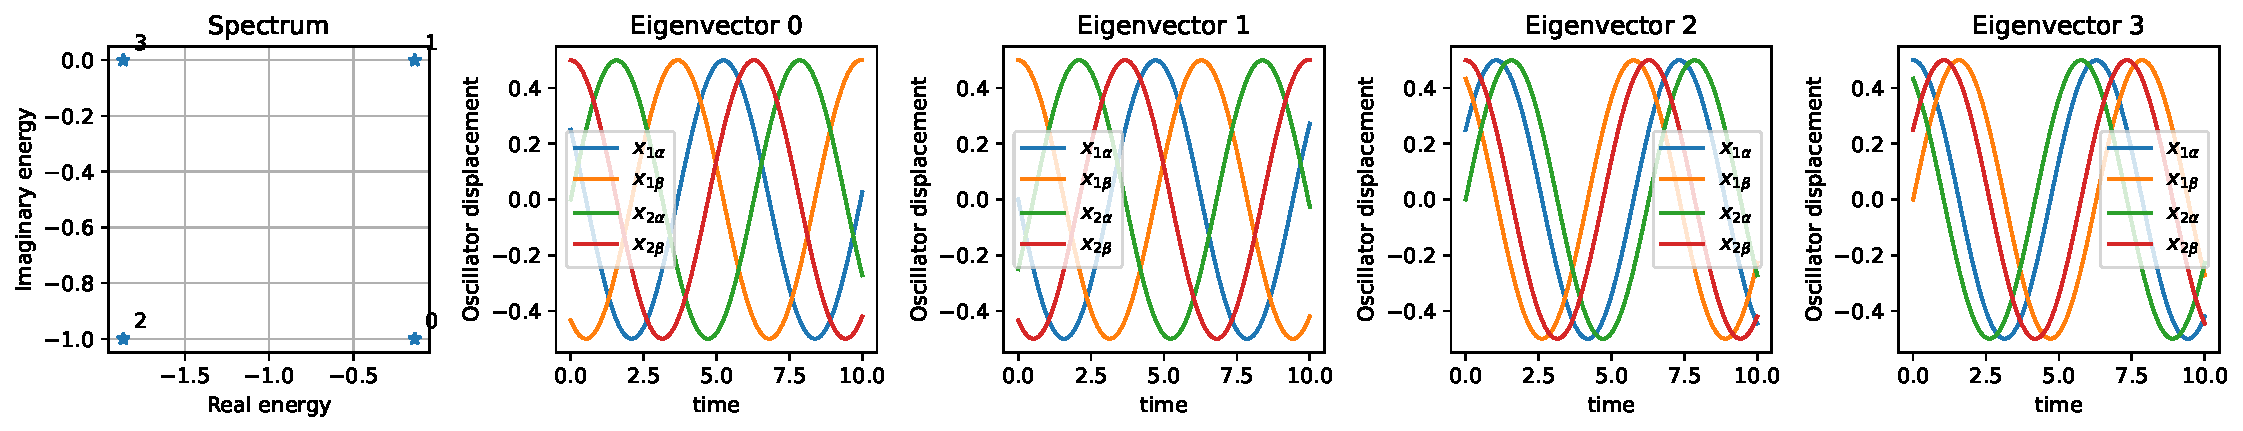
\includegraphics[width=\textwidth]{spectrum_2units_passive.pdf}
    \end{center} 
    \caption{} 
    \label{subfig:spectrum_2units_passive}
    \end{subfigure}
    \caption{\textbf{Spectrum and eigenvectors of linearized system of two coupled non-reciprocal units.}
    Each row has five panels. The first one is the spectrum in the complex energy plane. The rest are the eigenvectors 
    as a function of time. The displacement of each of the actuator is shown for each eigenvector. 
    The dominant eigenvector in the dynamics is the one with highest imaginary energy. 
    \textbf{\ref{subfig:spectrum_2units_same_chir}} Two active units with the same chirality. 
    \textbf{\ref{subfig:spectrum_2units_opp_chir}} Two active units with opposite chirality. 
    \textbf{\ref{subfig:spectrum_2units_passive}} One active and one passive units. 
    }
    \label{fig:spectrum_2units}
\end{figure}

Next we study the linearized dynamics. 
The spectrum and the time evolution of the eigenvectors are shown in figure \ref{subfig:spectrum_2units_same_chir}.
One can see that the spectrum forms a square in the complex energy plane. In other words, pairs of eigenvalues have the same real 
part and other pairs have the same imaginary part. The eigenmodes whose real energy is the lowest (2 and 3) have in-phase synchronized motion 
between the 2 oscillators, while the eigenmodes with the highest real energy (1 and 4) have an anti-phase synchronized motion.
The imaginary part of the energy also plays a role. Modes with positive imaginary energy are amplified and modes with negative 
imaginary energy are damped. Therefore, the mode with highest imaginary energy has the most amplification and it will dominate the 
dynamics. In figure \ref{subfig:spectrum_2units_same_chir}, the highest imaginary energy eigenvalue is the one labeled 2, 
and its mode corresponds to 
the actuators $1\alpha$ and $2\alpha$ oscillating $\pi/2$ ahead in phase in comparison to actuators $1\beta$ and $2\beta$. 
The mode corresponds to in-phase synchronized counterclockwise oscillations of the limit cycles. This the mode dominates the dynamics.
In comparison, mode 3 corresponds to clockwise oscillations. Its smaller value 
of imaginary energy makes it decay in time and have no appearance on the dynamics. The other mode with positive imaginary energy is 
eigenmode 0. It also corresponds to counterclockwise oscillations, but the limit cycles are antiphase rather than in-phase. It means 
that the phase difference between the limit cycles is $\pi$. Since this mode has slightly smaller imaginary energy and larger real energy, 
it is also obscured by the dominating mode.
This is what one could expect from intuition, but we still had to check it. By allowing the actuators to oscillate, 
it is energetically favourable for them to synchronize, and for them to have the same phase.

We can also compute the spectrum and eigenvectors of two units with opposite chirality. 
The results are shown in figure \ref{subfig:spectrum_2units_opp_chir}. As we said, the dynamics are dominated by the mode 
with highest imaginary energy. In the case of figure \ref{subfig:spectrum_2units_opp_chir}, those are modes 0 and 1. 
Mode 0 corresponds to large oscillations of the first unit, while the oscillations of the second unit are attenuated. 
For mode 1 the roles switch, so the second unit has larger amplitude. This means that units with opposite chirality 
do not oscillate simultaneously with large amplitude. They cancel each other's oscillations.
Consider also the case where the first unit is active and the right one is passive. 
The results for this configuration are shown in \ref{subfig:spectrum_2units_passive}. The dominant mode here is number 3. 
It corresponds to oscillations of the active unit, followed by the passive unit with a phase delay. This is 
precisely what we expected. The passive unit is dragged along by the active one. 
The phase delay comes from the time it takes the interaction to travel. That is given by the strength of 
the viscoelastic couplings $k_b$ and $k_v$. 

% \begin{figure}
%     \begin{center}
%     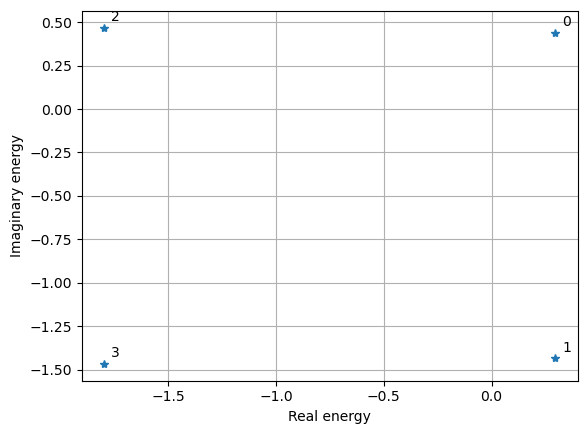
\includegraphics[width=0.5\textwidth]{2NR_coupled_pendula_spectrum.png}
%     \caption{Spectrum of 2 non-reciprocal coupled oscillators}
%     \label{2_sites}
%     \end{center}
% \end{figure}
% \begin{figure}
%     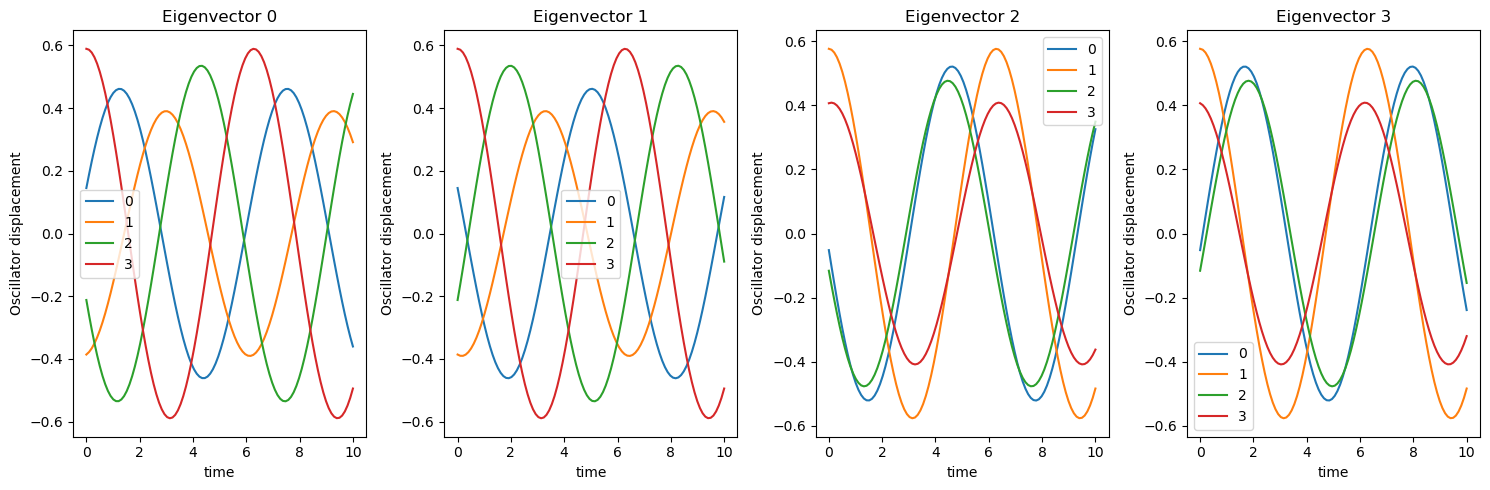
\includegraphics[height=3cm, width=\textwidth]{2NR_coupled_pendula_eigenvectors.png}
%     \caption{Time evolution of displacements for the different eigenvectors of 2 non-reciprocal coupled oscillators.}
%     \label{2_sites_eigenvectors}
% \end{figure} 
%What happens if one is passive? And if they have different chiralities?
% \begin{figure}
%     \begin{center}
%         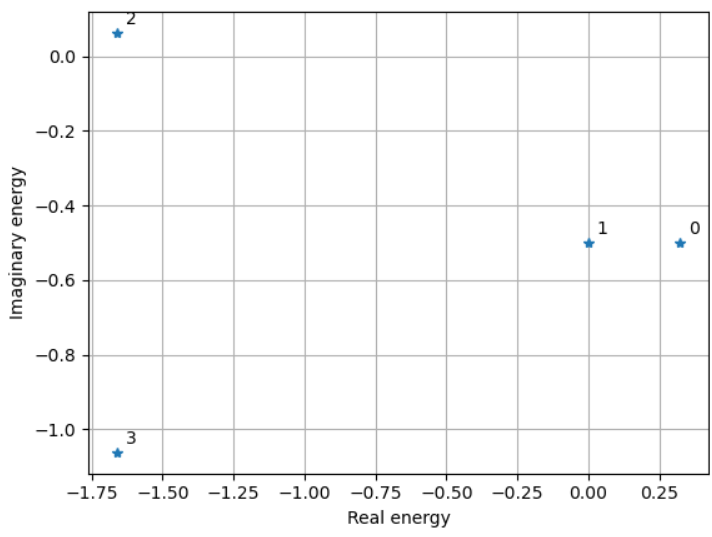
\includegraphics[width=0.5\textwidth]{2_osc_NR_and_pass_eigenvalues.png}
%     \end{center}
% \end{figure}
% \begin{figure}
%     \begin{center}
%         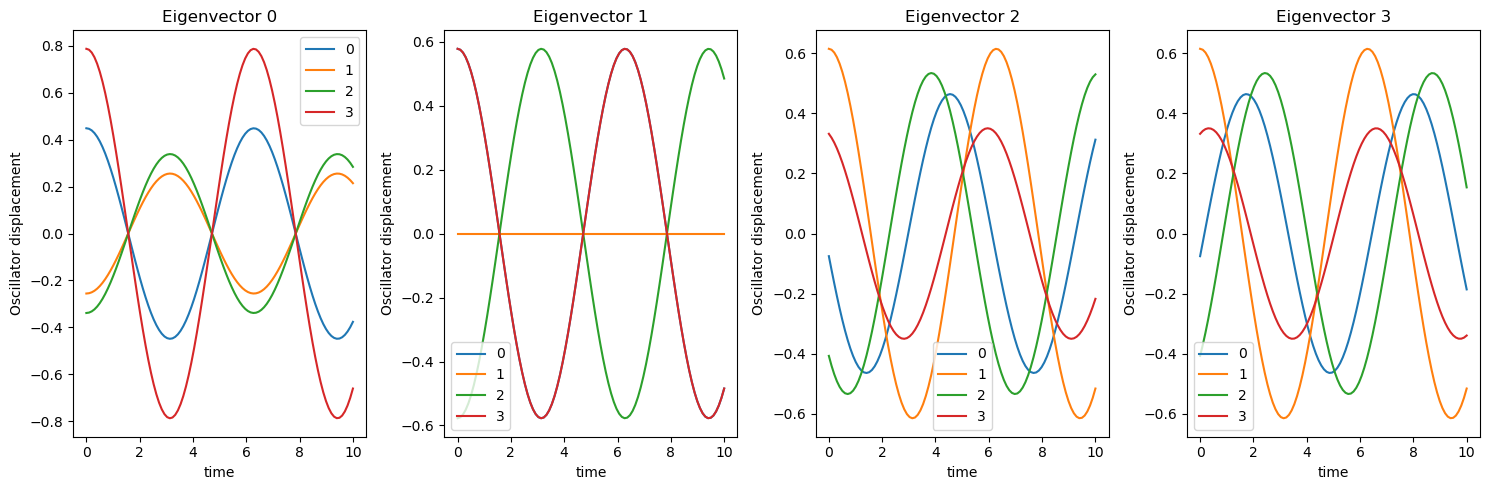
\includegraphics[width=\textwidth]{2_osc_NR_and_pass_eigenvectors.png}
%     \end{center}
% \end{figure}

% \subsection{Experiments with same chirality}
% \label{subsec:2units_exp_same_chir}

\subsection[Experiments with same chirality]{%
  Experiments with same chirality%
  \hspace{1cm}% Space between image and text
  \raisebox{-2cm}{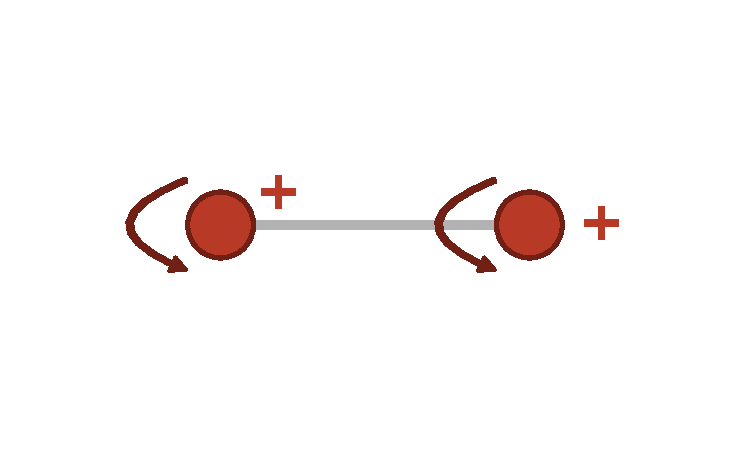
\includegraphics[scale=0.4]{diagram_2_units_same_chir_straight.pdf}}%
}
\label{subsec:2units_exp_same_chir}
% \begin{figure}
%     \begin{center}
%         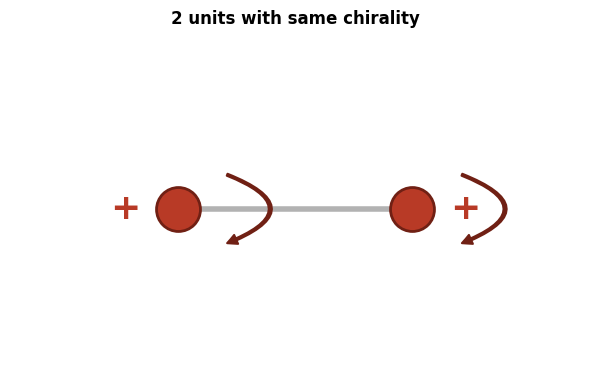
\includegraphics[width = 0.4\textwidth]{diagram_2_units_same_chir_straight.png}
%         \caption{fig}
%         \label{diagram_2_units_same_chir_straight}
%     \end{center}
% \end{figure}

We can study experimentally what happens when coupling two non-reciprocal oscillators. We place two non-reciprocal units 
in our wall setup, so 4 linear actuators in total, and the pairs are independent of one another. There is no interaction between 
the units. We did an experiment in which the non-reciprocal units had the same chirality, but 
were oscillating with different frequencies above the Hopf bifurcation. One of the nodes was oscillating with a frequency of $\SI{13.81}{Hz}$, 
and the other one with $\SI{14.61}{Hz}$. We then added a viscoelastic band coupling the two units together. The result of the coupling 
was that the nodes synchronized to the same frequency, which was measured to be $\SI{14.01}{Hz}$. These measurements showed 
a phenomenom of the system that I didn't anticipate: synchronization. In fact, the phenomenom is present all throughout the 
project. After some reading and thinking, the synchronization of non-reciprocal units is understood naturally. Each non-reciprocal 
unit performs a self-sustained limit cycle. When several of these units are coupled together, they will keep performing the 
limit cycle but they will also interact with one another. The interactions can cause phase delays and frequency shifts. 
In most cases, the most favourable mode of oscillation is the one in which they all oscillate with the same frequency and 
with very similar phase, since this mode minimizes the interactions thorugh the viscoelastic band. 

\begin{figure}
    \begin{center}
        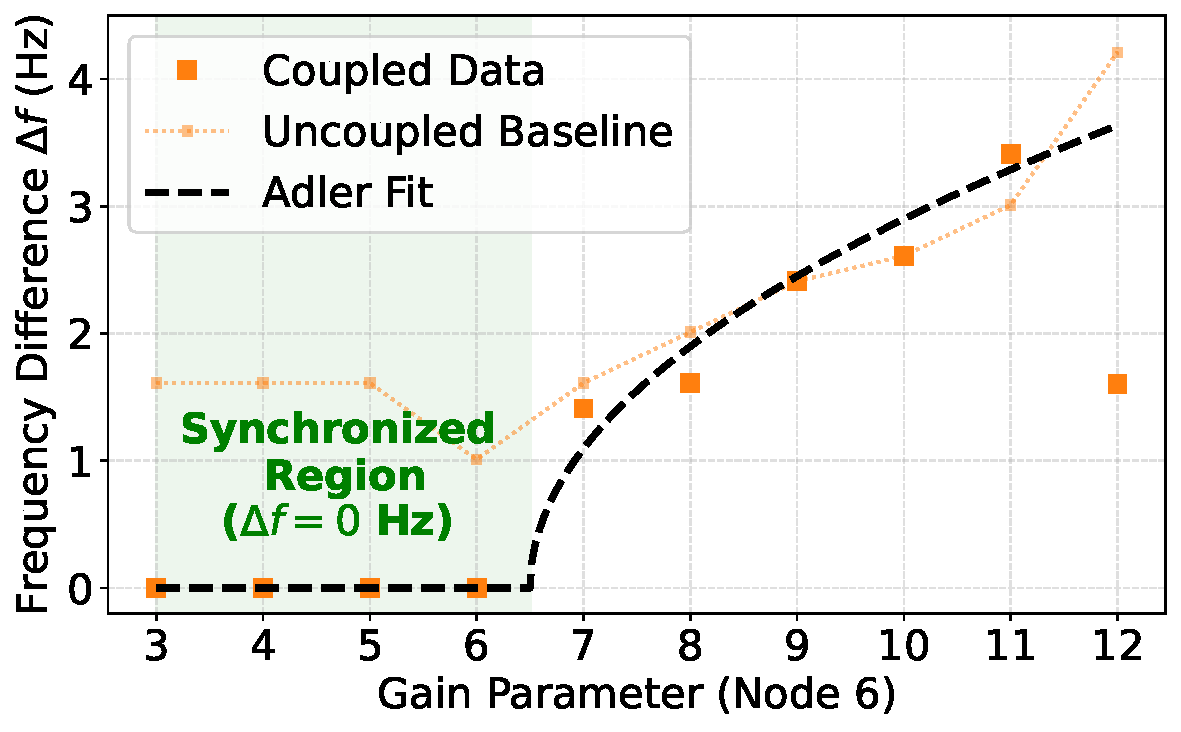
\includegraphics[width = 0.6\textwidth]{sync_region_freq_diff.pdf}
        \caption{\textbf{Synchronization region of two coupled units with the same chirality.} 
        The units are performing limit cycles, and they are coupled together via a viscoelastic band. We fix 
        one of the activity/gain parameters, and we vary the other one in the x-axis. We show the frequency difference 
        between the two units in the y-axis. The region where the frequency difference is zero corresponds to synchronization. 
        The other region where the frequency difference is nonzero corresponds to chaos. 
        The last data point (gain=12) of the coupled data is believed to be a consequence of oscillation quenching. }
        \label{2_nodes_same_chir_sync}
    \end{center}
\end{figure}

To study synchronization, we considered two units with the same chirality. We kept one of the unit's activity fixed during the whole experiment, 
$k_a = 7$ for node 4, and we varied the other unit's activity, node 6. That way we only had one parameter to change in the experiment. 
Figure \ref{2_nodes_same_chir_sync} shows the frequency of the limit cycles performed by the two units for different gain 
values of node 6. Node 4 data is drawn as circles and node 6 data as squares. For each activity value of node 6, we did 3 types of measurements. 
The first one was to determine the natural frequency of node 4 when it was oscillating by itself, and node 6 had zero activity. 
In the plot the data is shown as a soft circles. Since we didn't change its activity throughout the experiment, 
its frequency is constant. The second type of measurement is the natural frequency of node 6 when node 4 has zero activity. 
These data points are soft squares. The third type of measurement is both nodes having nonzero activity and coupled together 
by the viscoelastic band. This is the most relevant type of measurement, and it indicates whether the units synchronize or not. 
%The other type of measurements are just some baselines to compare. 
The data points for the frequency in this case are shown as solid or filled circles and squares. 
Since each unit is made out of two actuators, denoted L and R, there are double the number of data points. However, L and R 
are coupled non-reciprocally to form the limit cycles, and that forces them to already oscillate with the same frequency. 
Then, the corresponnding L and R data points coincide. 


Looking at the whole figure \ref{2_nodes_same_chir_sync}, there are two regions. For high activity parameter of node 6, 
the units oscillate with different frequencies. Therefore, the units are not synchronized in that region. 
For low activity values of node 6, in the range $k_a \in [3,6]$, the units do synchronize. The results are 
consistent with the theory. We saw that the synchronization of two oscillators can be described by the Adler equation.
If the coupling was larger than the detuning, then the oscillators synchronized. If the coupling 
was smaller than the detuning, then they didn't synchronize. These two regions are clearly visible in figure \ref{2_nodes_same_chir_sync}.
For $k_a \in [3,6]$, the oscillators synchronize, which means that the coupling is larger than the detuning. 
For $k_a \in [7,12]$, the oscillators don't synchronize, which means that the detuning is larger than the coupling.
However, the Adler equation cannot explain the whole plot. We observe that the detuning is the same for $k_a = 3,4,5,7$, 
but the units synchronize for $k_a = 3,4,5$ and they don't synchronize for $k_a = 7$. What has changed between the measurements? 
It is important to keep in mind that the only parameter we control is the activity of one of the units. As we saw in section 
\ref{sec:one_node_exp}, the activity of a unit affects both its natural frequency and its amplitude of oscillation. 
The detuning is not a variable we control directly, but we can control it indirectly through the activity. 
In experiments, the detuning can be easily measured by comparing the natural frequencies of the two units when they are uncoupled.
One might think that the coupling is constant, because the viscoelastic band remains unchanged in the experiment. 
However, we saw in section \ref{sec:one_node_exp} that the amplitude of oscillation of a unit depends on its activity.
%[maybe refer to specific equation and figure, and not section]
And in section \ref{subsec:1unit_theory}, we saw that the Kuramoto-like couplings between two non-reciprocal units depends 
on the amplitudes. Therefore, the coupling in the system is not constant and depends nontrivially on the activity. 
The Adler equation is derived by taking the phase dynamics approximation, which assumes that the amplitudes are constant. 
In the experimental setup of non-reciprocal actuators, the approximation does not hold if we change the activity, 
and so the results are not expected to be fully explained by the Adler equation. 


We observe that the frequency of node 6 grows linearly with its own activity in 
the uncoupled case. In the coupled case, after the units stop synchronizing, the coupled frequency of node 6 follows closely follows the 
uncoupled one. Therefore, after transitioning to the non-synchronized region, each unit oscillates with a frequency similar to 
the uncoupled one. The small coupling, in comparison with the detuning, has a small effect on the oscillation frequency in this region. 
We can also observe that as the detuning becomes larger, the effect of the coupling becomes smaller, and so the units 
oscillate with their natural frequencies. This observation can also be explained by the Adler equation, whose relevant 
parameter was the ratio of coupling to detuning. As the detuning increases, the effective coupling decreases. 
Nevertheless, for $k_a = 12$ something different happens. The frequency of node 6 drops substantially when coupling it to the other node. 
The data point might be a symptom of a phenomenom called oscillation quenching. %??? [check]
It could also be caused by the actuators oscillating erratically due to the large value of activity. In fact, we didn't 
take measurements for higher activity because we were afraid the actuators were going to break. 


\begin{figure}
    \begin{center}
        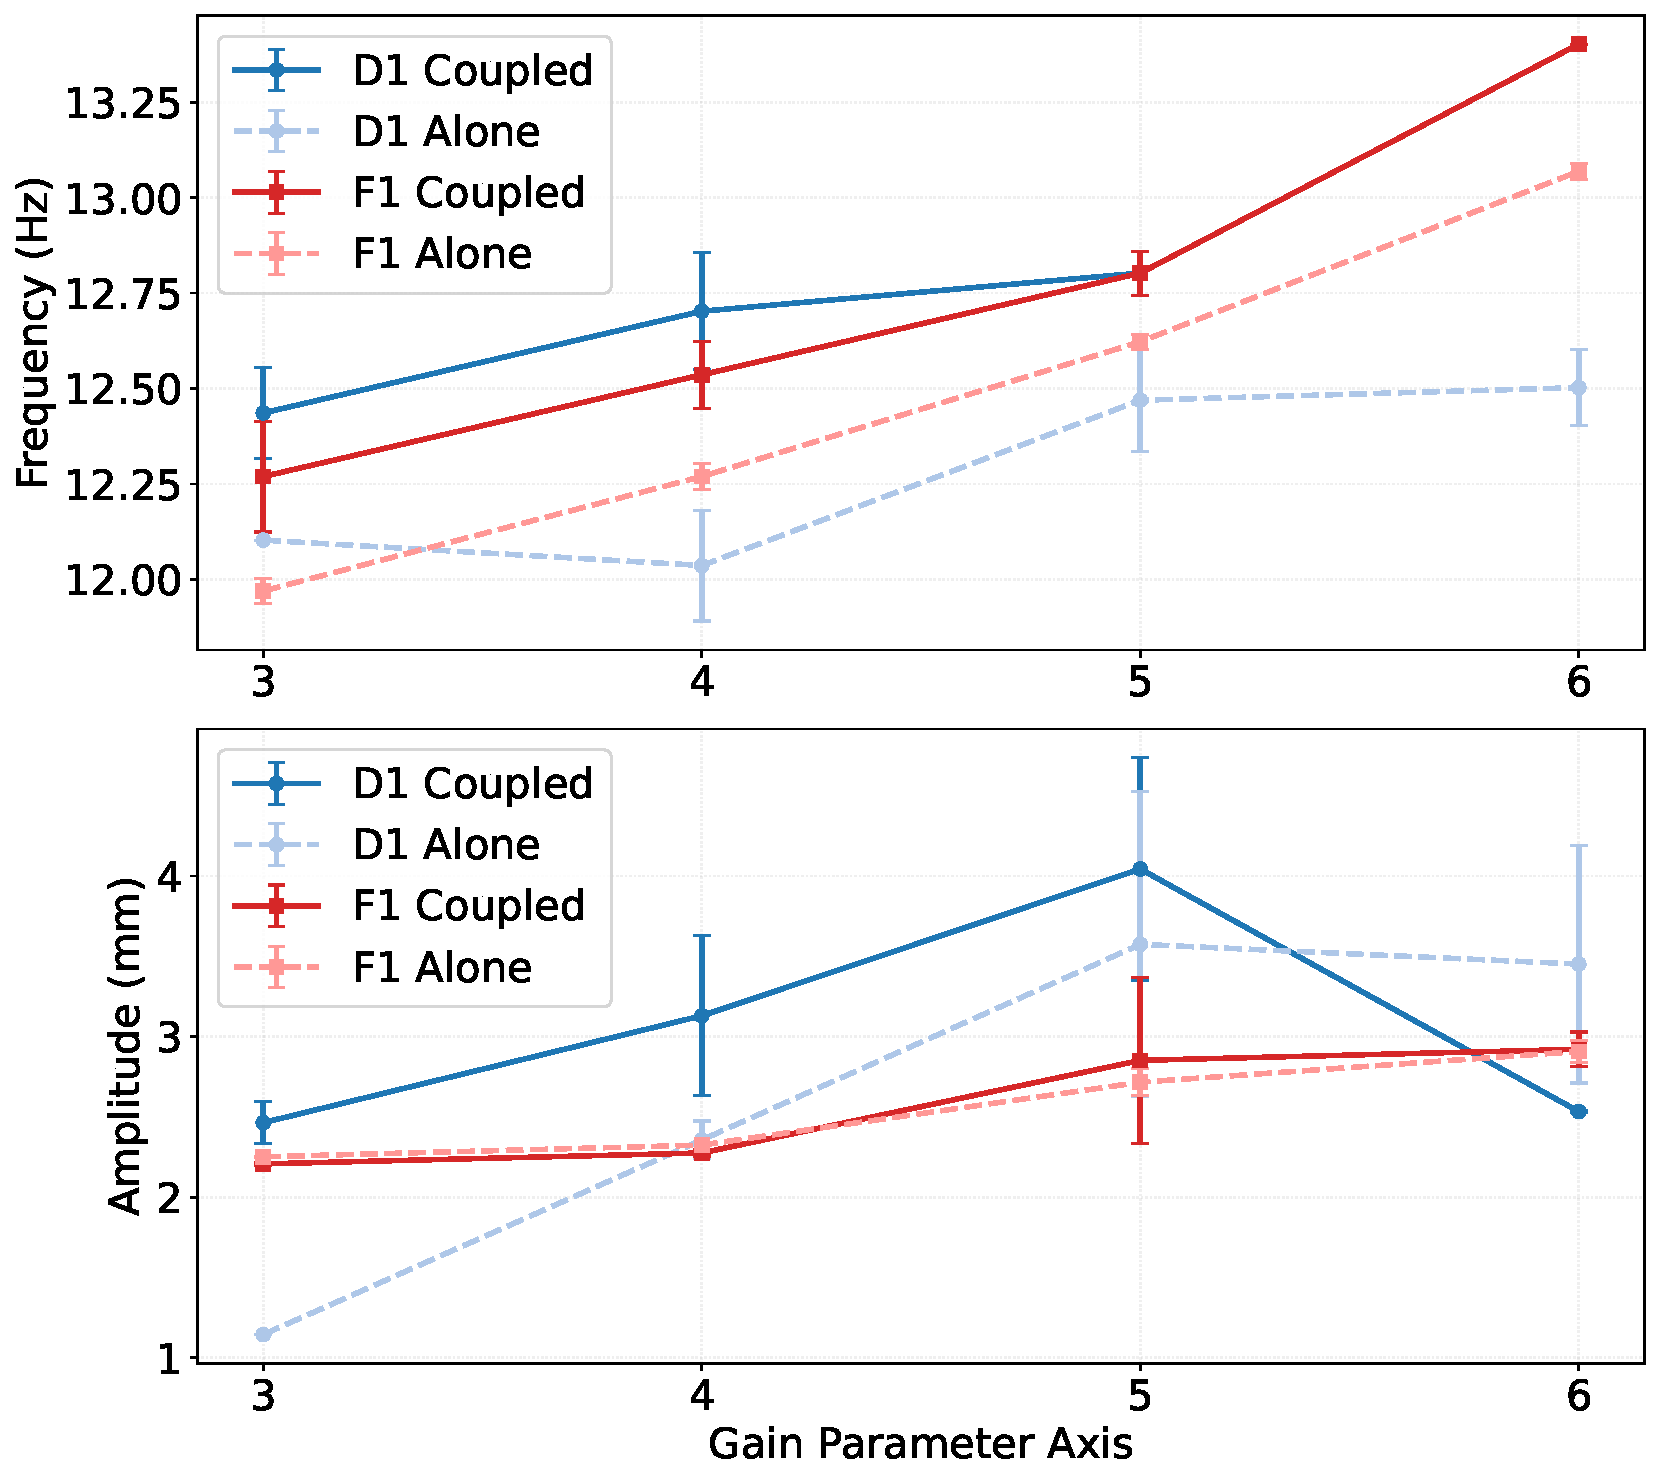
\includegraphics[width = 0.6\textwidth]{2_nodes_same_chir_repeated_2.pdf}
        \caption{\textbf{Experimental data of two coupled units with the same chirality. }
        The uncoupled/natural data is displayed by dash, dimmed lines. 
        The data taken when they are coupled is displayed in solid, colourful lines. 
        Different units are labeled with different colours. 
        The x-axis is the activity/gain parameter of the red unit (F1). The activity of the blue unit (D1) 
        is fixed to a constant value of $k_a^{\text{D1}}=6$. 
        \textbf{Top:} frequency of oscillations. \textbf{Bottom:} amplitude of oscillations. }
        \label{2_nodes_same_chir_sync_repeated}
        % change titile to frequnecy across activity of 2 nodes with same chirality
    \end{center}
\end{figure}

We wanted more reliable data, so we carried out another experiment in which we repeated each measurement 3 times. The actuators used 
were different to the previous experiment, so one cannot compare the specific details of the results. But using different actuators 
allows to distinguish what results are general and robust, and which are not. The results are shown 
in figure \ref{2_nodes_same_chir_sync_repeated}. Again, onne of the units had a fixed activity, in this case it was node D1 
with $k_a^{D1} = 6$ (shown in blue). The other unit's activity was varied, in this case it was node F1, shown in red. 
The soft dashed lines label the uncoupled data, while the solid colourful lines label the coupled data. 
Focusing first on the uncoupled frequencies, we observe that the frequency of unit F1 grows linearly when changing its 
activity. This is consistent with the results from the previous section and a good sanity check. 
Nevertheless, there is another sanity check that is not fulfilled. %[is this correct expression??]
Since we are only changing the activity of node F1, we expect the uncoupled frequency of node D1 to remain constant. 
Figure \ref{2_nodes_same_chir_sync_repeated} shows that it is not constant. Even though the measurements have 
large error bars, the frequency fluctuates and some results are incompatible. These fluctuations illustrate the 
poor quality of the actuators used in the experiment and the poor reproducibility of results. 
Although the results are not precise, making a quantitative analysis useless, we can still make some qualitative observations and conclusions. 


The first observation is that the units synchronize in most of the measurements. For $k_a^{F1} \in \{5,6\}$, 
the data points of both units coincide, so they clearly synchronize. 
For $k_a^{F1} \in [3, 4]$, the data points do not coincide. Note that the data points do not coincide 
because in one of the three trials, the units were not synchronized and oscillated with different frequency. Thus, 
it could be that the units did synchronize in other trials, since the error bars are compatible. And that is precisely
what one finds if one looks at individual trials. For $k_a^{F1} = 4$, the units synchronize in two trials and 
they don't synchronize in one of them. For $k_a^{F1} = 3$, the units synchronize in one trial and they don't synchronize in two of them.
Even in trials where the units did not synchronize, one can find periods of synchronization. And also, in trials 
where the units did synchronize, one can find phase slips. These observations can be seen in figure 
\ref{2_nodes_same_chir_repeated_phase} in the appendix \ref{subsec:annex_2units_same_chirality}, 
which shows the phase difference between the two units.

\subsection[Altermagnet unit cell]{%
  Altermagnet unit cell%
  \hspace{1cm}% Space between image and text
  \raisebox{-2cm}{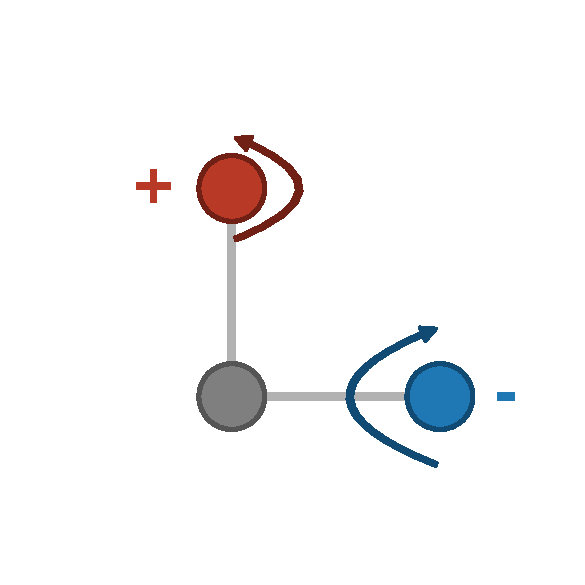
\includegraphics[scale=0.3]{diagram_2units_am_cell.pdf}}%
}
\label{subsec:2units_opp_chir}

% \begin{figure}[htbp]
%     \begin{center}
%         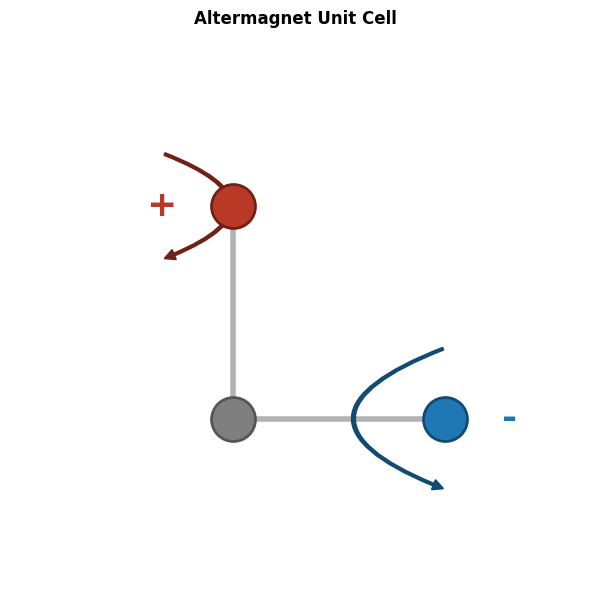
\includegraphics[width = 0.4\textwidth]{diagram_2units_am_cell.png}
%         \caption{fig}
%         \label{diagram_2units_am_cell}
%     \end{center}
% \end{figure}

We modified the previous configuration to units with opposite chirality. We also 
extended the system by adding a passive site and a mixture of horizontal and vertical couplings.
The motivation for this geometry is that it is precisely the unit cell of the 2D Lieb lattice.
We can consider coupling two units in an L shape, with opposite chirality, and adding a passive site 
in the vertex of the L. 
%The situation is sketched in figure \ref{diagram_2units_am_cell}. 
The passive site is mediating the interactions between the non-reciprocal units. In the experimental results of 
figure \ref{2_nodes_opp_chir_7-6-2026}, we fixed the gain of the negative-chirality unit (B5) to be $k_a^- = -7$, 
and we changed the gain of the positive-chirality unit (C4). The results for the frequency and amplitude 
are shown. Each data point is the average of 3 measurements. 
The error bars are the standard deviation of the 3 measurements. As before, 
the soft lines indicate the motion when the units are uncoupled, and the solid 
colourful lines when they are coupled. 
%Again, we see the frequencies of the units are similar to their natural frequencies when they are uncoupled.
What one observes in the frequency plot 
is that the units don't synchronize for any of the activity values. 
Even at the gain value of $k_a^+ = 7$, when their uncoupled frequencies are similar, 
further analysis shows that the units don't synchronize.
For $k_a^+ = 8$, the viscoelastic band coupling brings the frequencies closer together in 
comparison to the uncoupled case. This suggests that when the uncoupled frequency difference is small, 
there is an interaction between the units. The interaction tends to synchronize the units, 
but it doesn't succeed in doing so. We infer that synchronization doesn't 
happen when the units have opposite chirality. We run some simulations to test this hypothesis.

The observation can be explained with the Adler equation \eqref{eq:adler}. The first order approximation 
of the viscoelastic band coupling term is $\sim K\sin{\Delta\phi}$, as is shown in equation \eqref{eq_MSE_2nodes_phase}, 
which is derived in appendix \ref{subsec:2units_mse_derivation}. As the term originates from the viscoelastic band, 
it is expected to be equal for same and opposite chirality configurations. In contrast, the detuning 
significantly changes from one configuration to the other. In the case of two units with the same chirality, they have 
similar natural frequency, though not exactly equal. Therefore, the detuning is notably small: 
$\Delta \omega = \omega_2 - \omega_1 \ll \bigO(\omega_i)$. But in the case of two units with opposite chirality, 
one unit oscillates clockwise and the other counterclockwise. We can assign a sign to each of the directions, 
according to the chirality. This means that the natural frequencies actually have opposite signs, but are of the same 
order of magnitude. This means that the detuning is large: $\Delta \omega = \omega_2 - \omega_1 \sim  2\omega_i$. 
The Adler equation predicts that when the detuning is larger than the interaction coupling, then the units do not synchronize. 
This is precisely what we obtain in the experiments. If the units have the same chirality, the detuning is small, and they synchronize. 
If the units have opposite chirality, the detuning is large, and they don't synchronize. 

What we observed in simulations of two units with opposite chirality is that the units only synchronize if 
all the parameters are exactly the same. If the condition is not satisfied, then the units don't synchronize. The condition remains 
true for small and large values of gain. 
If the gain difference between the two units is not small, then the simulations show that the frequencies 
of oscillation in the coupled case are almost identical to the uncoupled case. The coupling 
has a very small effect and each unit follows their natural motion. 
If the gain difference is small, then the frequencies of oscillation drop considerably with respect to the 
uncoupled ones. In that case, both units oscillate with similar frequency, but not exactly the same. 
Also, the amplitude of oscillations in this case is reduced substantially with respect to the uncoupled case.

\begin{figure}[htbp]
    \begin{subfigure}[b]{0.48\textwidth}
        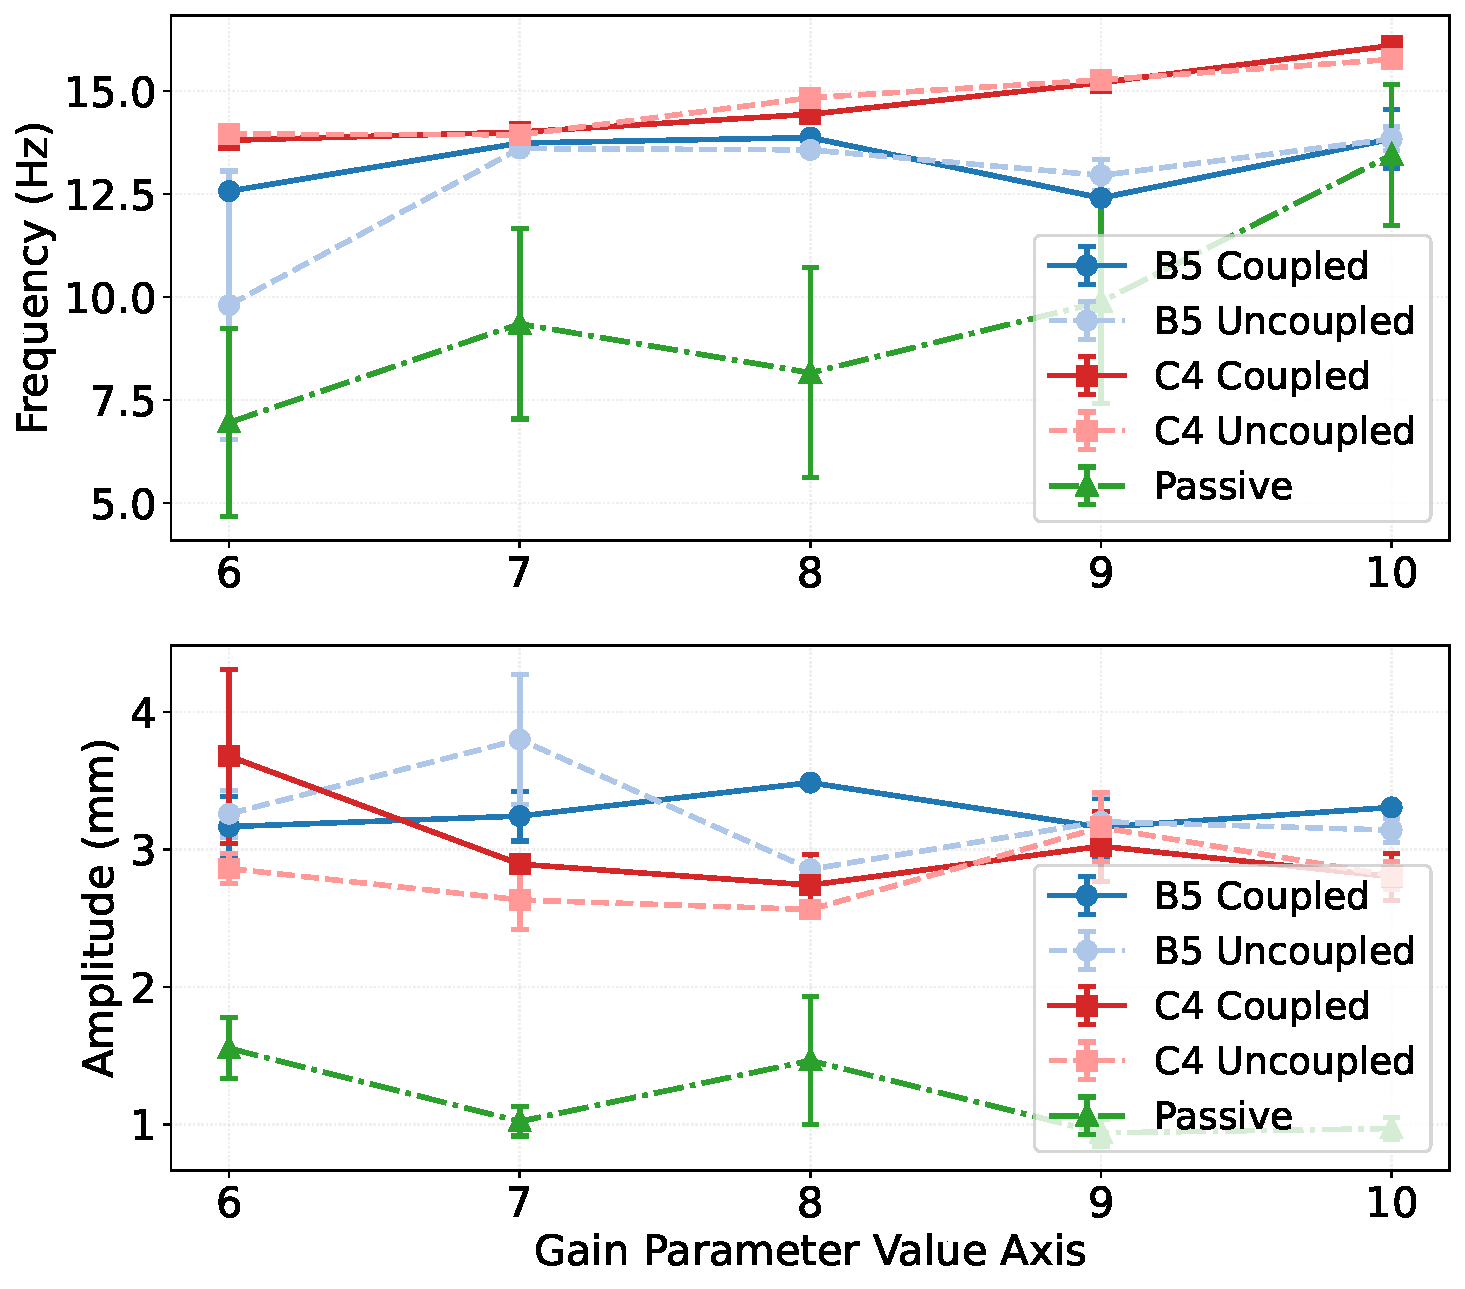
\includegraphics[width = \textwidth]{two_nodes_opp_chir_am_cell_sweep.pdf}
        \caption{}
        % \caption{\textbf{Experimental data of two coupled units with opposite chirality. }
        % The uncoupled/natural data is displayed by dashed, dimmed lines. 
        % The data taken when they are coupled is displayed in solid, colourful lines. 
        % Different units are labeled with different colours. 
        % The x-axis is the activity/gain parameter of the red unit (C4). The activity of the blue unit (B5) 
        % is fixed to a constant value of $k_a^\text{B5}=-7$. 
        % \textbf{Top:} frequency of oscillations. \textbf{Bottom:} amplitude of oscillations. }
        \label{2_nodes_opp_chir_7-6-2026}
    \end{subfigure}
    \begin{subfigure}[b]{0.48\textwidth}
    \centering
   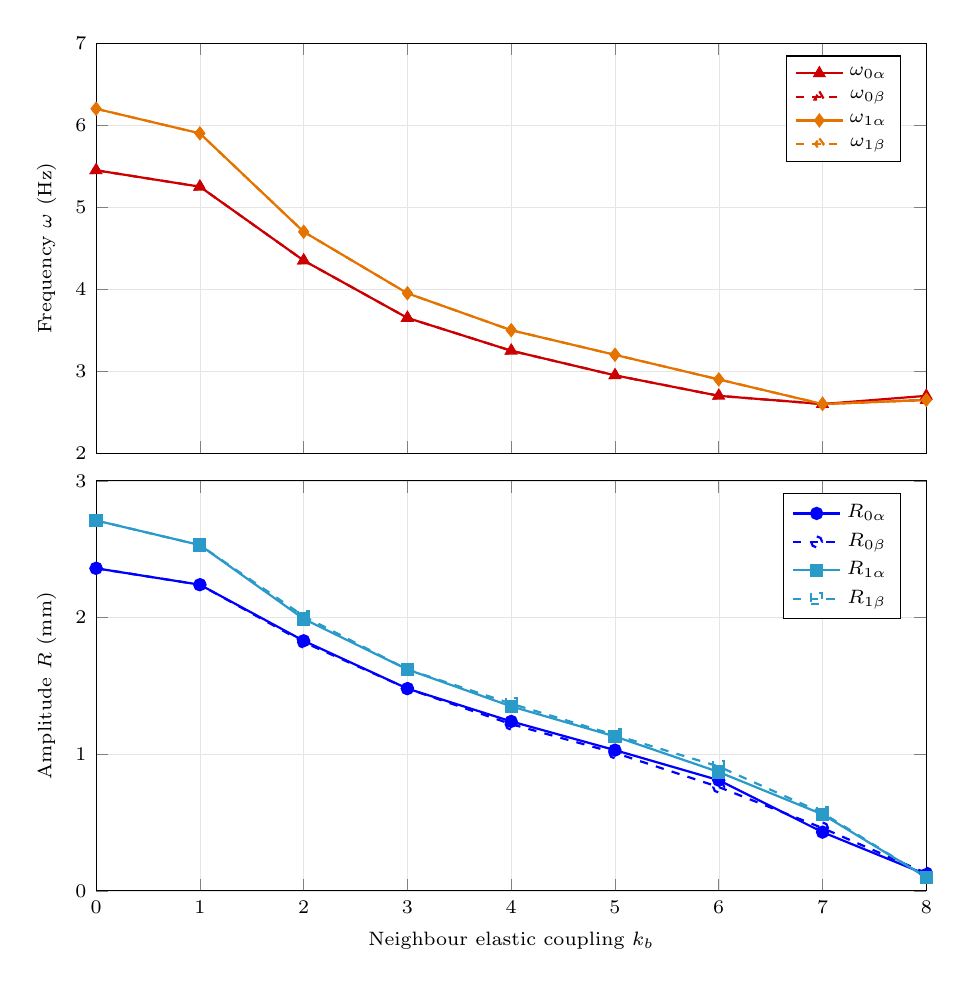
\begin{tikzpicture}
      \begin{groupplot}[
        group style={
          group size=1 by 2,
          vertical sep=0.35cm,
          x descriptions at=edge bottom
        },
        width=\linewidth,          % fit to subfigure width
        height=0.56\linewidth,     % reasonable aspect ratio
        xmin=0, xmax=8,
        xtick={0, 1, 2, 3, 4, 5, 6, 7, 8},
        grid=both,
        grid style={line width=.1pt, draw=gray!20},
        tick label style={font=\scriptsize},
        label style={font=\scriptsize},
        legend style={font=\scriptsize},
        title style={font=\scriptsize}
      ]

        % ================= TOP: FREQUENCIES =================
        \nextgroupplot[
          ylabel={Frequency $\omega$ (Hz)},
          ymin=2.0, ymax=7.0,
          legend pos=north east
        ]
          \addplot[thick, red!80!black, mark=triangle*] coordinates {
            (0, 5.45) (1, 5.25) (2, 4.35) (3, 3.65) (4, 3.25)
            (5, 2.95) (6, 2.70) (7, 2.60) (8, 2.70)
          };
          \addlegendentry{$\omega_{0\alpha}$}

          \addplot[thick, red!80!black, mark=triangle, dashed] coordinates {
            (0, 5.45) (1, 5.25) (2, 4.35) (3, 3.65) (4, 3.25)
            (5, 2.95) (6, 2.70) (7, 2.60) (8, 2.65)
          };
          \addlegendentry{$\omega_{0\beta}$}

          \addplot[thick, orange!90!black, mark=diamond*] coordinates {
            (0, 6.20) (1, 5.90) (2, 4.70) (3, 3.95) (4, 3.50)
            (5, 3.20) (6, 2.90) (7, 2.60) (8, 2.65)
          };
          \addlegendentry{$\omega_{1\alpha}$}

          \addplot[thick, orange!90!black, mark=diamond, dashed] coordinates {
            (0, 6.20) (1, 5.90) (2, 4.70) (3, 3.95) (4, 3.50)
            (5, 3.20) (6, 2.90) (7, 2.60) (8, 2.65)
          };
          \addlegendentry{$\omega_{1\beta}$}

        % ================= BOTTOM: AMPLITUDES =================
        \nextgroupplot[
          xlabel={Neighbour elastic coupling $k_b$},
          ylabel={Amplitude $R$ (mm)},
          ymin=0, ymax=3.0,
          legend pos=north east
        ]
          \addplot[thick, blue, mark=*] coordinates {
            (0, 2.36) (1, 2.24) (2, 1.83) (3, 1.48) (4, 1.24)
            (5, 1.03) (6, 0.81) (7, 0.43) (8, 0.12)
          };
          \addlegendentry{$R_{0\alpha}$}

          \addplot[thick, blue, mark=o, dashed] coordinates {
            (0, 2.36) (1, 2.24) (2, 1.82) (3, 1.48) (4, 1.22)
            (5, 1.01) (6, 0.76) (7, 0.46) (8, 0.13)
          };
          \addlegendentry{$R_{0\beta}$}

          \addplot[thick, cyan!80!black, mark=square*] coordinates {
            (0, 2.71) (1, 2.53) (2, 1.99) (3, 1.62) (4, 1.35)
            (5, 1.13) (6, 0.87) (7, 0.56) (8, 0.10)
          };
          \addlegendentry{$R_{1\alpha}$}

          \addplot[thick, cyan!80!black, mark=square, dashed] coordinates {
            (0, 2.71) (1, 2.53) (2, 2.01) (3, 1.62) (4, 1.37)
            (5, 1.14) (6, 0.91) (7, 0.57) (8, 0.10)
          };
          \addlegendentry{$R_{1\beta}$}

      \end{groupplot}
    \end{tikzpicture}
\caption{}
% \caption{\textbf{Simulation data of two coupled units with opposite chirality. }
% \textbf{Top:} Amplitude of oscillations of individual actuators in each unit, as the elastic coupling strength is varied. 
% \textbf{Bottom:} Frequency of oscillations of individual actuators in each unit, as the elastic coupling strength is varied. 
% The subscripts 0 and 1 denote the different units. The superscripts $a$ and $b$ denote the two actuators within each unit. }
\label{fig:kn_stacked_subplots}
\end{subfigure}
\caption{\textbf{Experimental and simulation data of two coupled units with opposite chirality. }
The configuration includes a passive site and both vertical and horizontal couplings, to reproduce the altermagnet unit cell.
\textbf{\ref{2_nodes_opp_chir_7-6-2026}} Experimental data of frequency (top) and amplitude of oscillations (bottom).
The uncoupled/natural data is displayed by dashed, dimmed lines. 
        The data taken when they are coupled is displayed in solid, colourful lines. 
        Different units are labeled with different colours. 
        The x-axis is the activity/gain parameter of the red unit (C4). The activity of the blue unit (B5) 
        is fixed to a constant value of $k_a^\text{B5}=-7$. 
\textbf{\ref{fig:kn_stacked_subplots}} Simulation data of frequency (top) and amplitude (bottom) of oscillations,
of individual actuators in each unit, as the elastic coupling strength is varied. 
The subscripts 0 and 1 denote the different units. The superscripts $\alpha$ and $\beta$ denote the two actuators within each unit. 
}
\label{fig:2units_opp_chir}
\end{figure}

We mentioned before that the experimental units are notably inhomogeneous in their properties. We model this observation in 
the simulation by introducing quenched disorder in all of the parameters. And we saw in the simulations the units with opposite 
chirality only synchonize if all the parameters are exactly the same. However, in the experiment we can control only the 
gain parameter, the rest of the parameters are fixed and unique for each unit. By the rest of parameters, we mean the 
linear, cubic spring constants and the damping coefficient. Therefore, even if we set 
exactly the same gain for the two units, the other parameters will be different, and that prevents the synchronization. 
In conclusion, units with oppposite chirality don't synchronize in general. 

The conclusion is also supported by the theoretical predictions. We can describe the phase difference of the two units as 
an Adler equation with higher order terms, which we can neglect in a first approximation. The condition of two units with 
opposite chiralities means that one unit has a positive oscillation frequency, i.e. the phase grows monotonically, and the 
other unit has a negative oscillation frequency, in the sense that the phase decreases monotonically. Therefore, the 
frequencies of the two units are roughly opposite of each other: $\omega_1 \sim -\omega_2$. Then, the detuning for 
opposite chirality is large $\Delta \omega \sim 2\omega_1$. It is much larger than any detuning encountered in the 
configuration of units with the same chirality. Since the coupling strength is similar to the one found in configuration 
of units with same chirality, the system with opposite chirality is in the region where $\Delta \omega > K$. The Adler 
equation predicts no synchronization, which agrees with the experiments and simulations. 

One might ask what the effect of adding the passive site and having both vertical and horizontal couplings were. 
These two modifications do not change the phenomena observed, hence the altermagnet unit cell has the same behaviour 
as two coupled units with opposite chirality. Analogously, the behaviour of a ferromagnet unit cell is qualitatively 
the same as the one of two coupled units with the same chirality. Thus, we skip the analysis of those configurations. 
The modifications do change the details of the results. For example, adding the 
passive site introduces more degrees of freedom and modes of oscillation that absorb energy from the active units. 
It makes the interaction strength between active units effectively smaller. As a consequence, if one couples two units with 
same chirality and introduces a passive site in between, the system requires a higher activity for the nodes to synchronize. 
At low values of activity, the passive site damps the displacement of the active ones, and the interaction is too 
small for there to be synchronization. Having both vertical and horizontal 
couplings of the viscoelastic band had no effect on the qualitative features of the system. The viscoelastic band still 
mediated the interactions, and change of direction did not matter. However, we did observe slight differences
in the results when coupling units in different directions. In order to study this asymmetry and the combination 
of different interactions, we consider in the next section a cross cell. 

\subsection{Simulations}
\label{subsec:2units_sim}

%First, we consider two units with same chirality. 
%\dots Mention parameters of simulation.


% \begin{figure}[htbp]
% \begin{tikzpicture}
%   \pgfplotsset{
%     scale only axis,
%     xmin=0, xmax=8,
%     xtick={0, 1, 2, 3, 4, 5, 6, 7, 8},
%     width=10.5cm, height=6cm
%   }

%   % =========================================================================
%   % LEFT Y-AXIS: RADIUS (mm)
%   % =========================================================================
%   \begin{axis}[
%     axis y line*=left,
%     xlabel={$k_b$},
%     ylabel={Radius $R$ (mm)},
%     ylabel style={blue!80!black},
%     yticklabel style={blue!80!black},
%     ymin=0, ymax=3.0,
%     grid=both,
%     grid style={line width=.1pt, draw=gray!20},
%     legend style={at={(0.03,0.97)}, anchor=north west, font=\small}
%   ]
%     % R0 (averaged where split)
%     \addplot[thick, mark=*, blue] coordinates {
%       (0, 2.36)
%       (1, 2.24)
%       (2, 1.825)
%       (3, 1.48)
%       (4, 1.23)    % Updated (R0_top=1.24, R0_bot=1.22)
%       (5, 1.02)
%       (6, 0.785)
%       (7, 0.445)
%       (8, 0.125)   % Updated (R0_top=0.12, R0_bot=0.13)
%     };
%     \addlegendentry{$R_0$}

%     % R1 (averaged where split)
%     \addplot[thick, mark=square*, cyan!80!black] coordinates {
%       (0, 2.71)
%       (1, 2.53)
%       (2, 2.00)
%       (3, 1.62)
%       (4, 1.36)    % Updated (R1_top=1.35, R1_bot=1.37)
%       (5, 1.135)
%       (6, 0.89)
%       (7, 0.565)
%       (8, 0.10)    % Updated (R1_top=0.10, R1_bot=0.10)
%     };
%     \addlegendentry{$R_1$}
%   \end{axis}

%   % =========================================================================
%   % RIGHT Y-AXIS: FREQUENCY (Hz)
%   % =========================================================================
%   \begin{axis}[
%     axis y line*=right,
%     axis x line=none, % Hide redundant x-axis
%     ylabel={Frequency $\omega$ (Hz)},
%     ylabel style={red!80!black},
%     yticklabel style={red!80!black},
%     ymin=0, ymax=7.0,
%     legend style={at={(0.03,0.73)}, anchor=north west, font=\small}
%   ]
%     % omega_0
%     \addplot[thick, dashed, mark=triangle*, red!80!black] coordinates {
%       (0, 5.45)
%       (1, 5.25)
%       (2, 4.35)
%       (3, 3.65)
%       (4, 3.25)    % Updated
%       (5, 2.95)
%       (6, 2.70)
%       (7, 2.60)
%       (8, 2.65)    % Updated (w0_top=2.70, w0_bot=2.65 -> mean=2.65)
%     };
%     \addlegendentry{$\omega_0$}

%     % omega_1
%     \addplot[thick, dashed, mark=diamond*, orange!90!black] coordinates {
%       (0, 6.20)
%       (1, 5.90)
%       (2, 4.70)
%       (3, 3.95)
%       (4, 3.50)    % Updated
%       (5, 3.20)
%       (6, 2.90)
%       (7, 2.60)
%       (8, 2.65)    % Updated (w1_top=2.65, w1_bot=2.65)
%     };
%     \addlegendentry{$\omega_1$}
%   \end{axis}

% \end{tikzpicture}
% \caption{Evolution of node radii ($R_0, R_1$) and frequencies ($\omega_0, \omega_1$) up to $k_b = 8$, clearly illustrating synchronization ($\omega_0 \approx \omega_1$) and radius decay past $k_b \ge 7$.}
% \label{fig:kn_sweep_plot_updated}
% \end{figure}
% \begin{figure}[htbp]
%     \centering
% \begin{tikzpicture}
%   \begin{groupplot}[
%     group style={
%       group size=1 by 2,       % 1 column, 2 stacked rows
%       vertical sep=0.5cm,      % Vertical spacing between plots
%       x descriptions at=edge bottom % Only show x-label/ticks on the bottom plot
%     },
%     width=11cm, height=5.5cm,
%     xmin=0, xmax=8,
%     xtick={0, 1, 2, 3, 4, 5, 6, 7, 8},
%     grid=both,
%     grid style={line width=.1pt, draw=gray!20},
%     legend style={font=\footnotesize}
%   ]

%     % =========================================================================
%     % TOP SUBPLOT: INDIVIDUAL RADII / AMPLITUDES
%     % =========================================================================
%     \nextgroupplot[
%       ylabel={Amplitude $R$ (mm)},
%       ymin=0, ymax=3.0,
%       legend pos=north east
%     ]
%       % R0 Top
%       \addplot[thick, blue, mark=*] coordinates {
%         (0, 2.36) (1, 2.24) (2, 1.83) (3, 1.48) (4, 1.24) (5, 1.03) (6, 0.81) (7, 0.43) (8, 0.12)
%       };
%       \addlegendentry{$R_0^a$}

%       % R0 Bottom
%       \addplot[thick, blue, mark=o, dashed] coordinates {
%         (0, 2.36) (1, 2.24) (2, 1.82) (3, 1.48) (4, 1.22) (5, 1.01) (6, 0.76) (7, 0.46) (8, 0.13)
%       };
%       \addlegendentry{$R_0^b$}

%       % R1 Top
%       \addplot[thick, cyan!80!black, mark=square*] coordinates {
%         (0, 2.71) (1, 2.53) (2, 1.99) (3, 1.62) (4, 1.35) (5, 1.13) (6, 0.87) (7, 0.56) (8, 0.10)
%       };
%       \addlegendentry{$R_1^a$}

%       % R1 Bottom
%       \addplot[thick, cyan!80!black, mark=square, dashed] coordinates {
%         (0, 2.71) (1, 2.53) (2, 2.01) (3, 1.62) (4, 1.37) (5, 1.14) (6, 0.91) (7, 0.57) (8, 0.10)
%       };
%       \addlegendentry{$R_1^b$}


%     % =========================================================================
%     % BOTTOM SUBPLOT: INDIVIDUAL FREQUENCIES
%     % =========================================================================
%     \nextgroupplot[
%       xlabel={$k_b$},
%       ylabel={Frequency $\omega$ (Hz)},
%       ymin=2.0, ymax=7.0,
%       legend pos=north east
%     ]
%       % omega_0 Top
%       \addplot[thick, red!80!black, mark=triangle*] coordinates {
%         (0, 5.45) (1, 5.25) (2, 4.35) (3, 3.65) (4, 3.25) (5, 2.95) (6, 2.70) (7, 2.60) (8, 2.70)
%       };
%       \addlegendentry{$\omega_0^a$}

%       % omega_0 Bottom
%       \addplot[thick, red!80!black, mark=triangle, dashed] coordinates {
%         (0, 5.45) (1, 5.25) (2, 4.35) (3, 3.65) (4, 3.25) (5, 2.95) (6, 2.70) (7, 2.60) (8, 2.65)
%       };
%       \addlegendentry{$\omega_0^b$}

%       % omega_1 Top
%       \addplot[thick, orange!90!black, mark=diamond*] coordinates {
%         (0, 6.20) (1, 5.90) (2, 4.70) (3, 3.95) (4, 3.50) (5, 3.20) (6, 2.90) (7, 2.60) (8, 2.65)
%       };
%       \addlegendentry{$\omega_1^a$}

%       % omega_1 Bottom
%       \addplot[thick, orange!90!black, mark=diamond, dashed] coordinates {
%         (0, 6.20) (1, 5.90) (2, 4.70) (3, 3.95) (4, 3.50) (5, 3.20) (6, 2.90) (7, 2.60) (8, 2.65)
%       };
%       \addlegendentry{$\omega_1^b$}

%   \end{groupplot}
% \end{tikzpicture}
% \caption{\textbf{Simulation data of two coupled units with opposite chirality. }
% \textbf{Top:} Amplitude of oscillations of individual actuators in each unit, as the elastic coupling strength is varied. 
% \textbf{Bottom:} Frequency of oscillations of individual actuators in each unit, as the elastic coupling strength is varied. 
% The subscripts 0 and 1 denote the different units. The superscripts $a$ and $b$ denote the two actuators within each unit. }
% \label{fig:kn_stacked_subplots}
% \end{figure}

We consider two units with opposite chirality. We fix the activity of the units to $[7, -8]$, 
and saw the effect of changing the neighbour coupling $k_b$ in the dynamics. There are three regions. If 
$k_b \sim \bigO(0.1)$ is small, then the interaction is very small and the oscillators move independently. If $k_b \sim \bigO(1)$, 
the amplitudes of oscillations are modulated periodically. As the coupling is increased further, the amplitude 
decreases to zero. 

Next, we fixed the neighbour coupling to be $k_b=10$ and changed the values of activity of both units. 
If the activities were exactly opposite one of the other, then the oscillations cancel each other out. 
The displacements are very small. To compensate for it, we increase the activity of both units in magnitude, 
but keeping them opposite to each other. What we find are still small oscillations, but of same order of 
magnitude to the previous simulations. Surprisingly, the units synchronize. However, the synchronization is 
not robust under small disorder in the other parameters. This explains why in the experimental setup, in 
which there are imperfections in the actuators, we did not observe synchronization between two units with 
opposite chirality. 
If the activities are slightly different in magnitude, the simulation shows that the units do not synchronize. 
When the units are uncoupled, the limit cycles have different natural frequencies and different natural amplitudes. 
When coupling them together, the dynamics alternates through periods of large and small amplitudes. This is shown 
as a modulation of the oscillations of individual springs. The modulation is periodic, but in a timescale 
much larger than the period of oscillation. The modulation is caused by the phase difference 
between the two units. If the phase difference is far from being zero, then the oscillations are not canceled much,
so the units oscillate with considerably large amplitude. But when the phase difference between the units is close 
to zero, then the cancellation is much greater, and the amplitude is reduced. Since they do not synchronize, the 
phase difference is always increasing in time, and therefore we get alternating periods of large and small amplitude. 
The period of the modulation is then related to how different the magnitudes of activity are. If the activities 
are just slightly different, the period of modulation is very large, around $T_\text{mod}\sim \SI{30}{s}$, while the 
fast oscillations are order $T_\text{fast}\sim \SI{0.1}{s}$. For arbitrary different activities, we observe a 
modulation of $T_\text{mod}\sim \SI{10}{s}$. If one keeps making the activity difference even bigger, 
one actually encounters another case, besides synchronization, when two units with opposite chirality have no modulation. 
It happens when the activities are so different between each other that the natural frequencies are multiples of each other. 

\section{1D chain}
\label{sec:chain}

\subsection{Theory}
\label{subsec:chain_theory}

Before going to the Lieb lattice in 2D, we wanted to get intuition on a 1D system, a chain,
both classically and quantum mechanically. Classically just means considering the sites as oscillators coupled with springs, 
and quantum mechanically as sites with hopping amplitudes. 

Let's first consider the quantum case. We studied the Hatano-Nelson chain \cite{Hatano_1996}, with some added twists.
First, we stacked 2 chains on top of each other. We did this to have a two-level system per site and to be able to try different symmetries.
And second, we added non-hermiticity, in two ways. The first way is adding an imaginary onsite potential. 
The second way is adding non-reciprocal hoppings. The spectrum and the eigenstates are shown in the annex. 
Note that as we are now dealing with a non-Hermitian system whose behaviour is going to be sensitive to the boundary conditions we choose. 
As a consequence, we have to study the spectrum and eigenstates with both periodic and open boundary conditions. 

One of the things that stands out from the results is the symmetry that the spectrum manifests. 
We can observe that the spectrum displayed in the complex energy plane is symmetric with respect to the real and imaginary axes. 


%%%%%%%%%%%%%%%%%%%%%%%%%%%%%%%%%%%%%%%%%%%%%%%%%%%%%%%%%%%%%% Theory continuum 
We now show the analytic results of the theoretical approach in the specific case of a one-dimensional chain. 
For simplicity, we assumed that the neighbour coupling between units is linear.
We already know that the two actuators making up the unit will have a phase difference of $\Delta\phi=\pm\frac{\pi}{2}$, 
and so the odd elastic term in equation \eqref{eq_MSE_2nodes_phase} will vanish. 
By taking the mentioned simplifications in equation \eqref{eq_MSE_2nodes_phase}, we arrive at
the equation describing the phase dynamics of one quadrature-phase unit with neighbours:
\begin{equation}
    \dot{\phi}_i =  \omega_i + \frac{3k_{c}}{2\omega} R_i^2 + \sum_{<j>} \frac{k_v}{2}\left(\frac{R_j}{R_i}\sin{(\phi_j - \phi_i)} - 1\right) 
    + \sum_{<j>} \frac{k_b}{2\omega}\left(1 - \frac{R_j}{R_i}\cos{(\phi_j - \phi_i)}\right).
    \label{eq_phase_chain_discrete}
\end{equation}
For very long chains of identical oscillators, we can take the continuum approximation. Since the units have the 
same activity, we can assume that their amplitudes are fixed to the same value. The only degree of freedom left then 
is the phase. Since we are considering a one-dimensional chain, each unit has two nearest neighbours: one to the left and one to the right.
Thus, the sums in equation \eqref{eq_phase_chain_discrete} are made up of two addends. 
We expand in Taylor series only the last two terms, since they are the ones that include phases from different units. 
Using $\sin{\Delta\phi}\simeq \Delta\phi$, we simplify the viscous neighbour coupling term to be
$ \frac{k_v}{2}\left(\phi_{i-1} + \phi_{i+1} - 2\phi_i - 2\right)$. This is precisely the 
discrete second derivative of $\phi$, when one takes the distance between units $l$ to zero.
And using $\cos{\Delta\phi}\simeq 1 - \Delta\phi ^2$, we simplify the elastic neighbour coupling term to be 
$\frac{k_b}{2\omega}\left[(\phi_{i-1} - \phi_i)^2 + (\phi_{i+1} - \phi_i)^2\right]$. This is the gradient of the phase squared. 
The resulting continuum equation is the PDE:
\begin{equation}
    \frac{\partial \phi}{\partial t} = \underbrace{\omega + \frac{3k_{c}}{2\omega} R^2 + k_v}_{\Omega} + \frac{k_vl^2}{2}\nabla^2 \phi 
    + \frac{k_bl^2}{2\omega}\left(\nabla\phi\right)^2
    \label{eq_KPZ_phase_identical}
\end{equation}
The first three terms are constant, the fourth is diffusive and the fifth one is nonlinear. 
Formula \eqref{eq_KPZ_phase_identical} is the deterministic Kardar-Parisi-Zhang equation \cite{KPZ}. 
If equation \eqref{eq_KPZ_phase_identical} only had the first constant terms, all the phases increase homogeneously 
in time: $\phi(x,t) \approx \Omega t$. This is expected, as the units are autonomous oscillators. 
We now focus on the effect of the diffusive term. We disregard the rest. By expanding in Fourier modes, 
we find that the phase field can be written as
\begin{equation}
    \phi(x,t) \approx \sum_k c_k e^{-\frac{k_vl^2}{2}k^2 t + ikx}.
\end{equation}
We notice that each mode decays with a time constant (or mean lifetime) $\tau = \frac{2}{k_vl^2k^2}$.
The decay rate depends on the wavevector. 
For short wavelength modes, the decay is very fast. Longer wavelength modes have a slower decay rate. %($k\rightarrow 0$)
What we expect to happen in the dynamics is that the phase field becomes progressively smoother as time evolves. 
The short wavelength fluctuations die before the long wavelength fluctuations. At the end, only the $k=0$ mode survives, 
in which the phase field is constant in space. The diffusive term synchronizes the oscillators locally. 
The observable result is that the wavelength of the system increases in time. The end result is the synchronization of the 
whole chain. This phenomenom is called wave coarsening \cite{veenstra}. 
The nonlinear term has the opposite effect. It makes the gradients grow, so it can lead to the 
formation of kinks or fronts. 
The deterministic KPZ equation can be transfomed into the heat equation by a Cole-Hopf transformation. 
Therefore, we expect diffusion to dominate for long times. In fact,
the steady state solution of the heat equation with open boundary conditions is homogeneous. 
Since our field is the phase, this is equivalent to synchronization. 

There is a synchronization timescale, or in other words, a diffusion timescale for the phase. 
It is given by the slowest decaying mode: $k_1 = \frac{2\pi}{L}$, where $L$ is the lenght of the whole chain. 
We obtain a synchronization timescale of 
\begin{equation}
    \tau_{\text{sync}} = \frac{L^2}{2\pi^2 k_v l^2}.
    \label{eq:sync_timescale}
\end{equation}
We observe that it scales with the square of the system size. In consequence, longer chains take longer to synchronize. 


\subsection{Experiment}
\label{subsec:chain_exp}

We prepared an experimental configuration of a one-dimensional chain. Since each unit has two actuators, there are actually 
two chains, one to each side of the wall. The configuration had 7 units in total, 3 of which were active. 

% \begin{wrapfigure}{l}{0.2\textwidth}
%   \centering
%   % Make the graphic take up 90% of the wrapped box
%   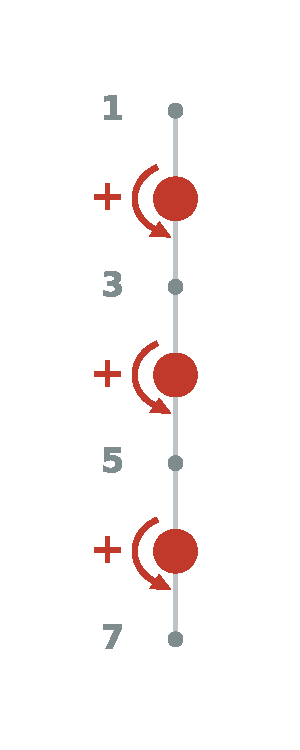
\includegraphics[width=0.9\linewidth]{diagram_chain_same_chir.pdf}
%   \caption{}
%   \label{fig:diagram_chain_same_chir}
% \end{wrapfigure}
At first, we set the active units to have the same chirality and studied the regime above the Hopf bifurcation. 
The spatio-temporal plot is shown in figure \ref{kymograph_same_chir_1dstrip}. Since the different colours indicate 
opposite displacements, the figure shows that there are oscillations in both the left and right actuators. If one plots the state 
space of each unit, the trajectory are the limit cycles we have discussed. The important feature of this figure is that the red 
and blue stripes are roughly vertical. That shows that the limit 
cycles in the steady state are phase-locked. They are oscillating with the same frequency and practically in-phase. There are 
slight differences in the phase, and the reason is that the active units drag the passive ones along with them. Therefore, the passive 
units (1,3,5,7) have their oscillations slightly delayed with respect to the active ones. In summary, a one-dimensional chain with 
the same chirality synchronizes, even if passive sites are added in between. 

\begin{figure}[htbp]
  \centering
  \begin{subfigure}[c]{0.2\textwidth}
    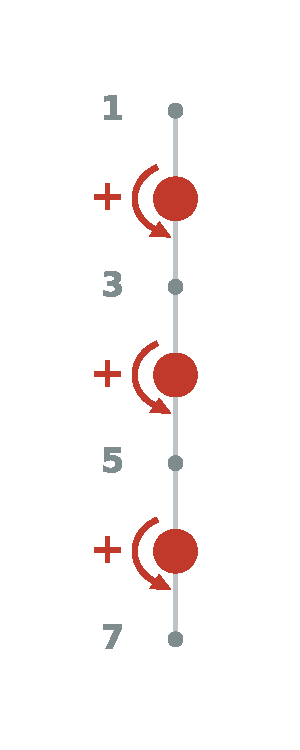
\includegraphics[height=6cm]{diagram_chain_same_chir.pdf}
    \caption{}
    \label{fig:diagram_chain_same_chir}
  \end{subfigure}
  \begin{subfigure}[c]{0.2\textwidth}
    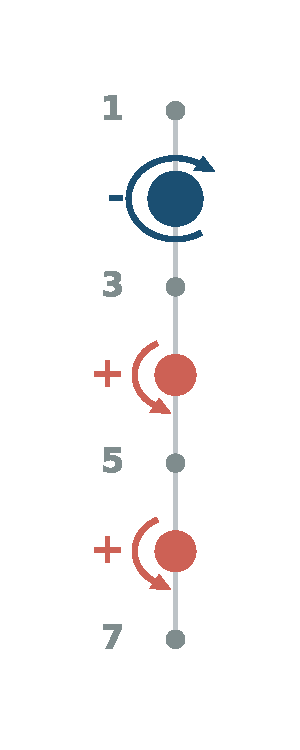
\includegraphics[height=6cm]{diagram_chain_opp_chir_2.pdf}
    \caption{}
    \label{fig:diagram_chain_opp_chir_2}
  \end{subfigure}
  \begin{subfigure}[c]{0.2\textwidth}
    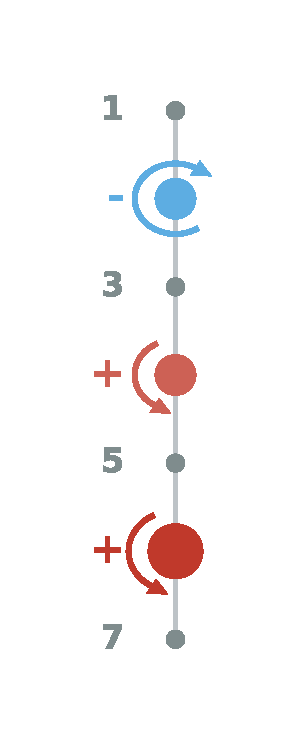
\includegraphics[height=6cm]{diagram_chain_opp_chir_6.pdf}
    \caption{}
    \label{fig:diagram_chain_opp_chir_6}
  \end{subfigure}   
  \caption{\textbf{Diagrams of the three configurations considered for the experiments in a 1D chain of units.}
  The red circles denote active units with positive chirality. The blue circles denote units with negative chirality. 
  The grey dots denote passive units. The strength of the activity parameter is highlighted by bigger and more intense circles. 
  \textbf{\ref{fig:diagram_chain_same_chir}} Chain with positive-chirality units, and passive sites in between. 
  \textbf{\ref{fig:diagram_chain_opp_chir_2}} The second unit has negative (opposite) chirality with high activity. 
  \textbf{\ref{fig:diagram_chain_opp_chir_6}} Similar configuration to \ref{fig:diagram_chain_opp_chir_2}, but now 
  the sixth unit has the highest activity. 
  }
  \label{fig:1d_chain_diagrams}
\end{figure}

Again, the reason why we observe synchronization 
is because we are in the regime after the Hopf bifurcation. The units trace out limit cycles, and that means that the oscillators are 
autonomous. Before the Hopf bifurcation, the units exhibit damped oscillations. The one-dimensional chain can host waves that 
propagate and attenuate. This regime was difficult to access experimentally, so we studied it using simulations (see section \ref{subsec:chain_sim}).

% \begin{wrapfigure}{l}{0.2\textwidth}
%   \centering
%   % Make the graphic take up 90% of the wrapped box
%   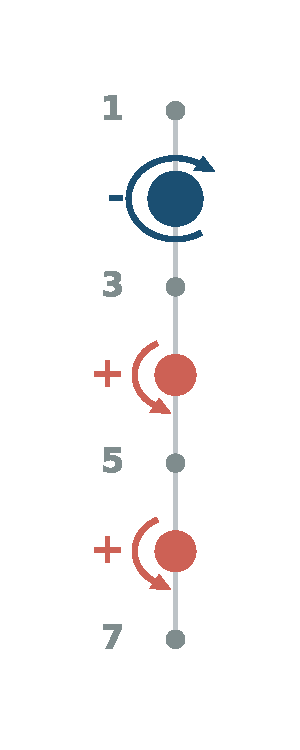
\includegraphics[width=0.9\linewidth]{diagram_chain_opp_chir_2.pdf}
%   \caption{}
%   \label{fig:diagram_chain_opp_chir_2}
% \end{wrapfigure}
We also carried out experiments where one of the units, specifically the second one, had the opposite chirality. This change results 
in a considerable reduction of the amplitude of oscillations of the actuators. In order to counteract the effect, we increased 
the activity of the opposite-chirality unit. The corresponding spatio-temporal plot is shown in \ref{kymograph_opp_chir_1dstrip_2}. In contrast to the chain with 
the same chirality, the system does not have an homogeneous appearance. In the figure, the actuators of the first three units display 
strong colours, while the rest of the figure gradually becomes white. Stronger colours mean that the amplitude of oscillations is large 
and white means that the amplitude is close to zero. As the second unit has the highest activity, we can think of it as the leader of 
the oscillations. The passive neighbour unit 1 follows the motion of the leader. However, the units with positive chirality cannot 
synchronize to the motion of the negative chirality unit. As they have lower activity in comparison, their oscillations are attenuated. 
In fact, the right actuators of units 3 and 4 are oscillating anti-phase with respect to unit 2. 

% \begin{wrapfigure}{l}{0.2\textwidth}
%   \centering
%   % Make the graphic take up 90% of the wrapped box
%   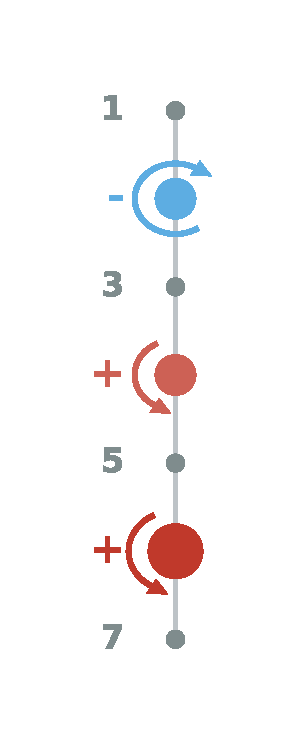
\includegraphics[width=0.9\linewidth]{diagram_chain_opp_chir_6.pdf}
%   \caption{}
%   \label{fig:diagram_chain_opp_chir_6}
% \end{wrapfigure}
We can carry out another experiment in which unit 6 has the highest activity. The spatio-temporal plot is shown in \ref{kymograph_opp_chir_1dstrip_6}. 
In this case, the amplitude is large for unit 6, small for units 5 and 4, and practically zero for the rest. Since the 
oscillations are damped, we observe diagonal strips of red and blue, rather than the vertical strips of panel \ref{kymograph_same_chir_1dstrip}. 
The diagonal stripes represent that the phase difference btween the units is nonzero. 
Unit 6 generates waves that propagate through the chain and attenuate at the same time. 

%In other experiments with very high activity and no passive springs, the active nodes []
%[mention the effect of having the passive springs]

All things considered, we observed spin-momentum locking in the one-dimensional chain. Placing units with the same chirality 
leads to synchronization with a large oscillation amplitude. In contrast, placing units with opposite chirality reduces 
significantly the amplitude, prohibiting the propagation of waves. 

%%%%%%%%%%%%%%%%%%%%%%%%%%%%%%%%%%%%%%%%%%%%%%%%%%%%%%%%%%%%%%%%%%%%%%%%%%%%%%%%%%%%%%%%%%%%%%%%%%%%%%
We started by building 2 chains of actuators, one chain to each side of the wall. % as seen in figure ??. 
Actuators that are symmetric with respect to reflection of the wall can be coupled non-reciprocally. % (maybe easier way to explain). 
In general, we won’t choose all actuators to be non-reciprocally 
coupled for geometric reasons. The actuators within the same chain are coupled mechanically via 
a viscoelastic band. 
%Keep in mind that the main goal is the study of the 2-dimensional altermagnet, so the 1-dimensional setup is just an intermediate step. 

In the first set of experiments, we had 3 PCBs that would control 3 non-reciprocal units. We had the option to add passive springs 
in between the active ones. We wanted to observe the same phenomena we had seen in the simulations, namely, spin-momentum locking. 
%We also wanted to analyse all the details of the system. 
5%To observe the spin-momentum locking, 
At first, all active nodes were set with the same chirality. The spatio-temporal plot 
(or kymograph) of figure \ref{kymograph_same_chir_1dstrip} shows that the nodes synchronize. 
However, when we flip the chirality of one of the nodes, the synchronization is lost. In fact, the actuators' oscillation attenuate 
as can be seen in figure \ref{kymograph_opp_chir_1dstrip_2}. 
This is a demonstration of the spin-momentum locking. If the nodes have the same chirality/pseudospin, then 
they synchronize and can be used to send waves (maybe). If they have opposite chirality/pseudospin, the oscillations 
die and there is no wave propagation.

\begin{figure}
    \begin{subfigure}{0.32\textwidth}
        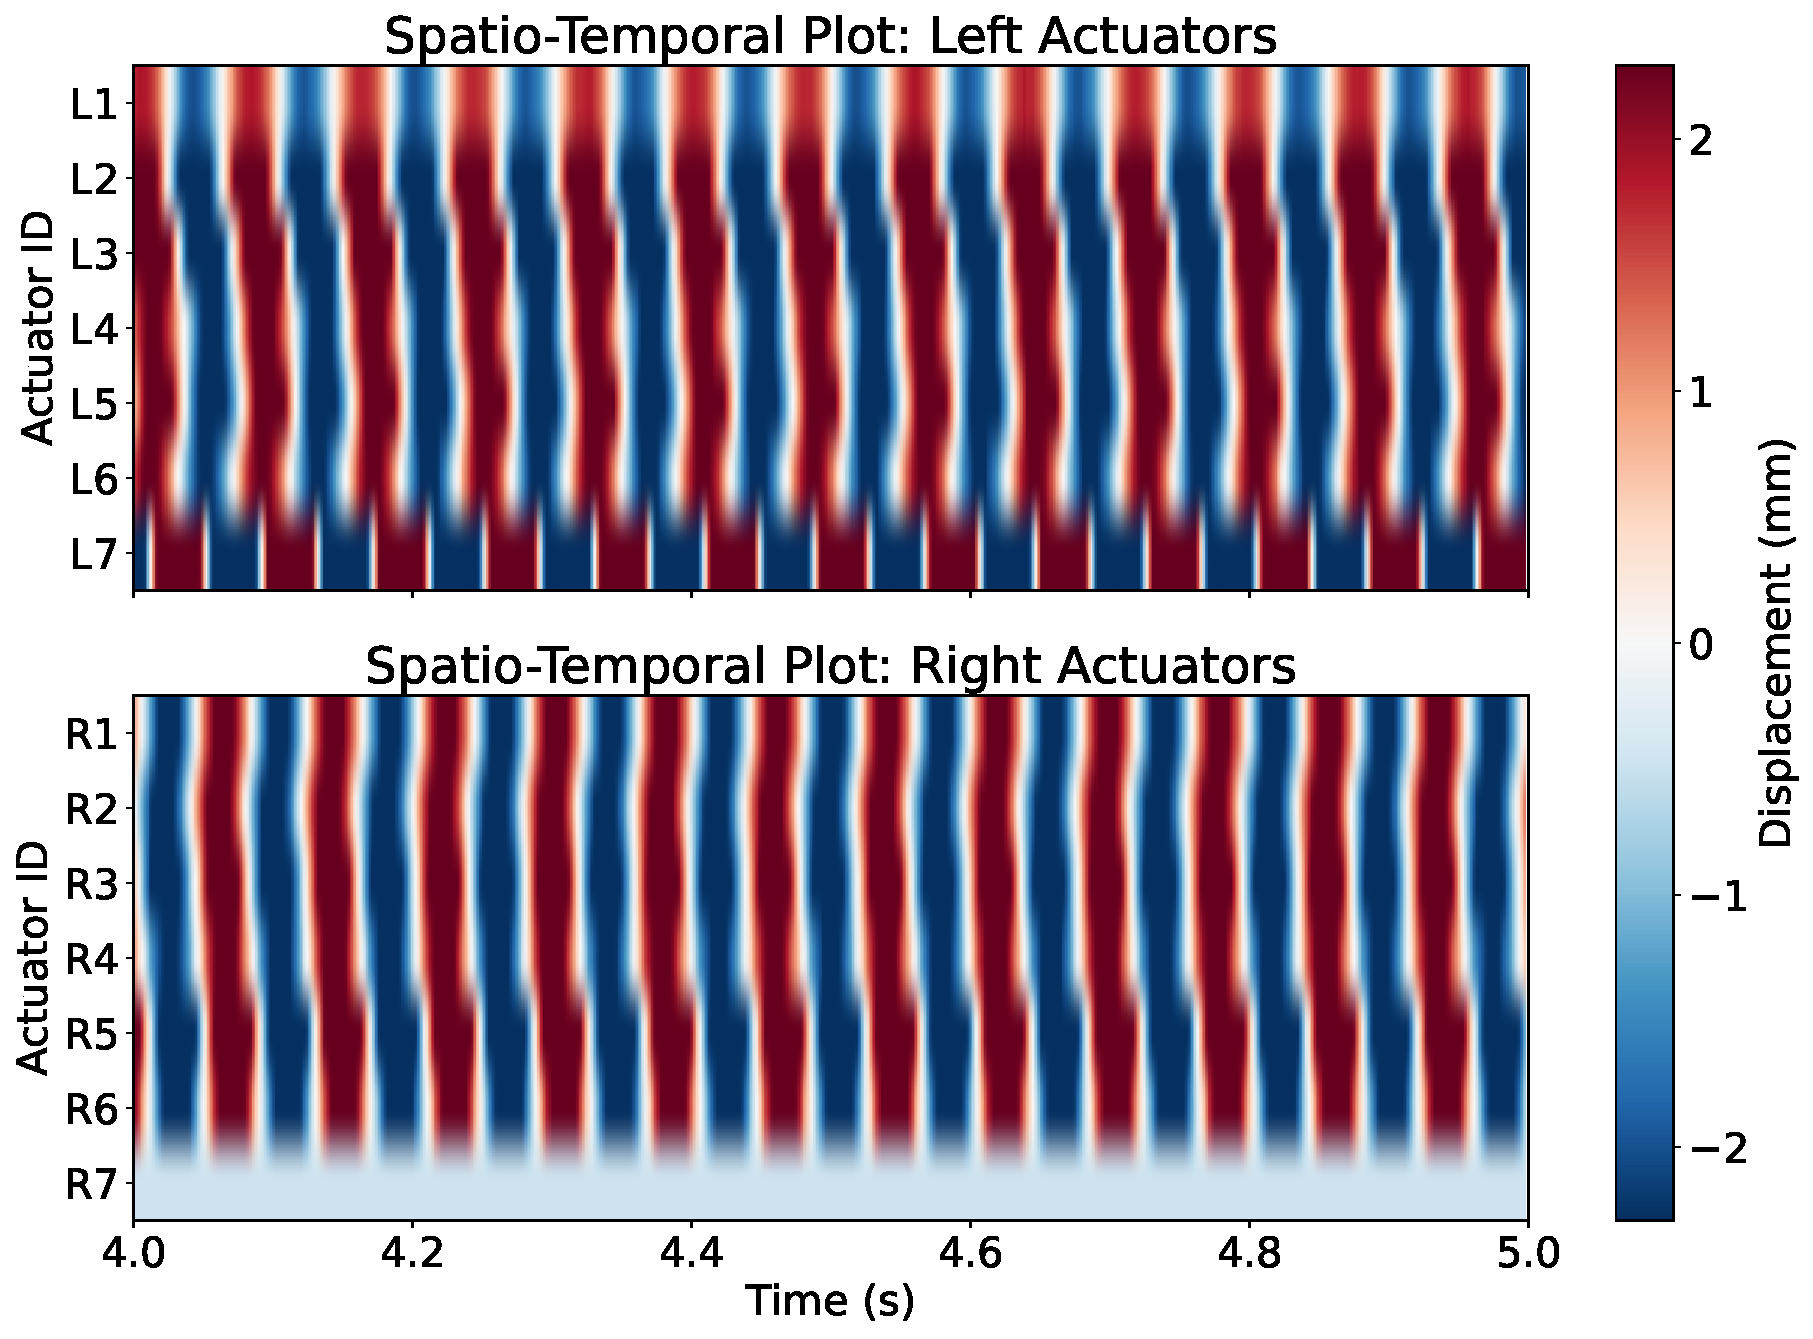
\includegraphics[width=\textwidth]{chain_same_chir.pdf}
        \caption{}
        \label{kymograph_same_chir_1dstrip}
    \end{subfigure}
    \begin{subfigure}{0.32\textwidth}
        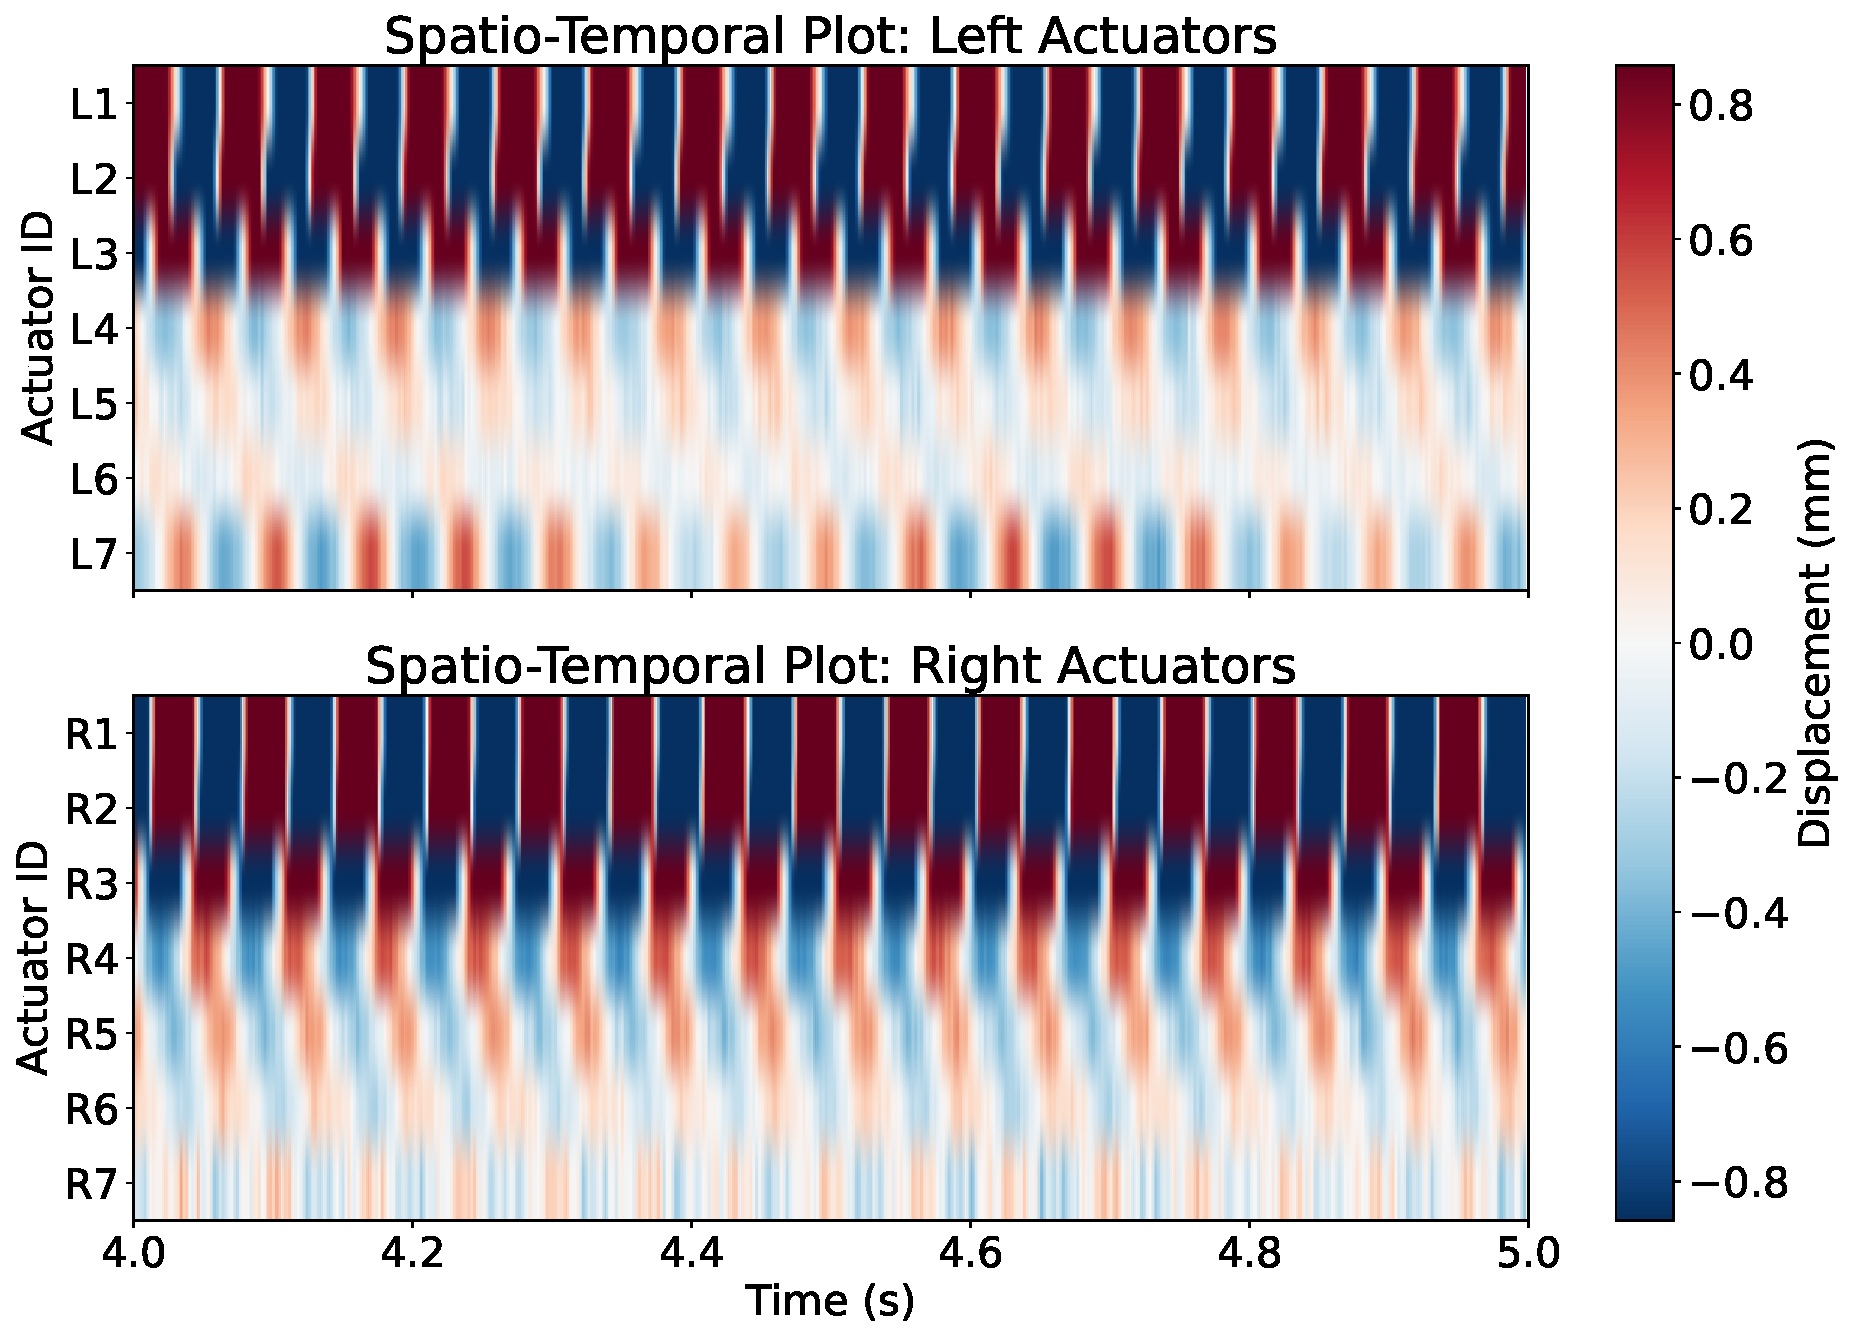
\includegraphics[width=\textwidth]{chain_opp_chir_2.pdf}
        \caption{}
        \label{kymograph_opp_chir_1dstrip_2}
    \end{subfigure}
    \begin{subfigure}{0.32\textwidth}
        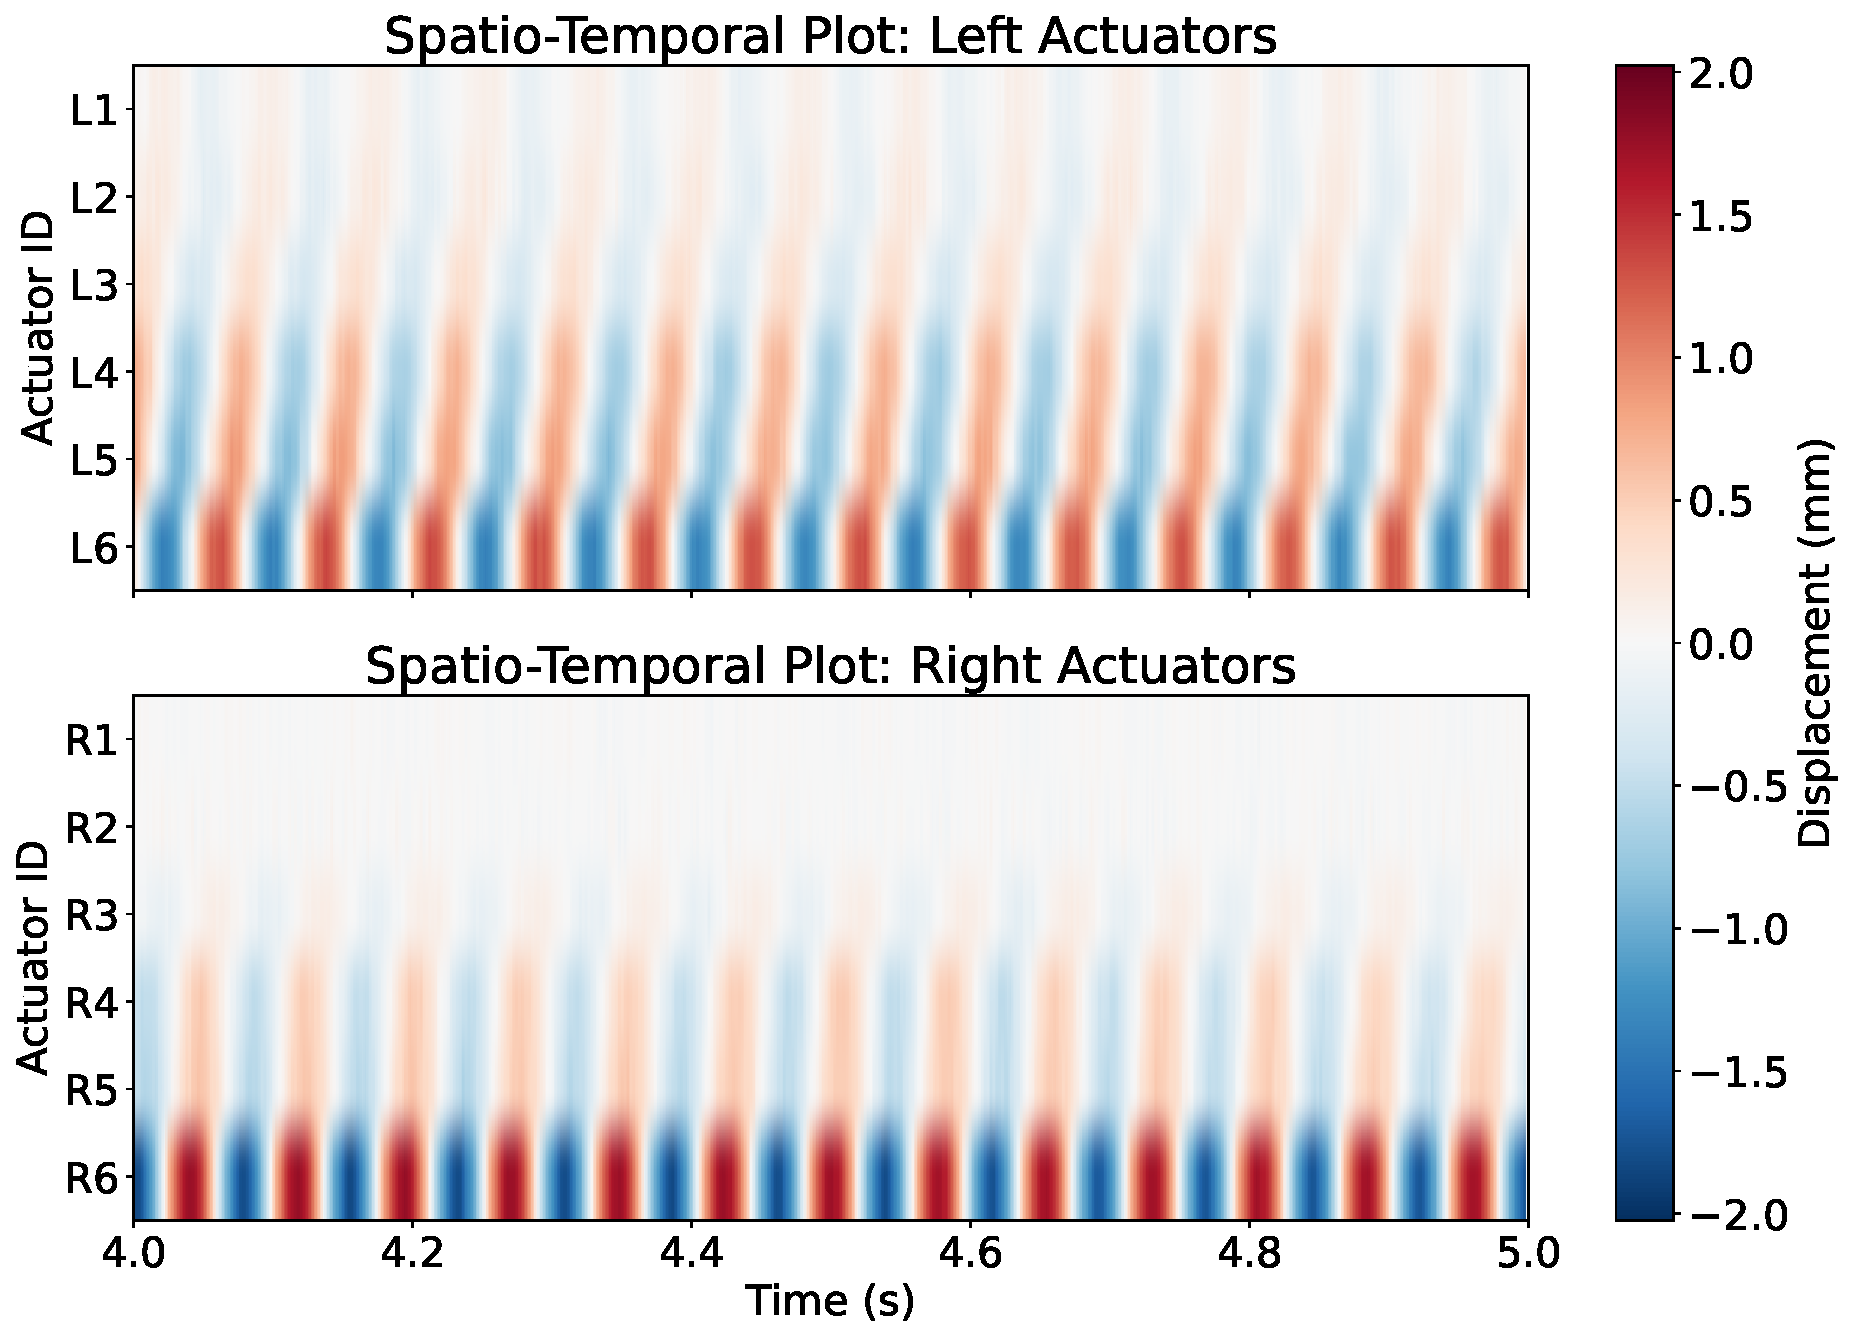
\includegraphics[width=\textwidth]{chain_opp_chir_6.pdf}
        \caption{}
        \label{kymograph_opp_chir_1dstrip_6}
    \end{subfigure}
    \caption{\textbf{Spatio-temporal plots of the 1D chain. }
    Each panel corresponds to the diagrams in figure \ref{fig:1d_chain_diagrams}. The top plot shows the displacement 
    of the left actuators (one side of the chain), while the bottom plot shows the displacement of the right actuators (other side of chain).
    \textbf{\ref{kymograph_same_chir_1dstrip}} Kymograph of the 1D strip with all nodes having the same chirality. 
    \textbf{\ref{kymograph_opp_chir_1dstrip_2}} Kymograph of the 1D strip with node 2 having highest activity 
    and opposite chirality to nodes 4 and 6. 
    \textbf{\ref{kymograph_opp_chir_1dstrip_6}} Kymograph of the 1D strip with node 6 having highest activity.}
\end{figure}


\subsection{Simulations}
\label{subsec:chain_sim}

We also run simulations of the 1D chain of actuators. One important difference
of the simulations with respect to the experiment, is that we assume the neighbour 
coupling is linear instead of cubic. The geometric structure of the chain is the same as the experimental one.
There are two chains of linear actuators, one on top of the other, that oscillate perpendicular to the direction of the chain. 
Each actuator on one chain has a corresponding partner in the other chain, and they are both on the same chain site. 
The actuator partners interact non-reciprocally, while the closest neighbours within the chain interact mechanically through 
the viscoelastic band. 
The parameters of the simulation are: 
\begin{itemize}
    \item Number of nodes
    \item Onsite stiffness / natural frequency
    \item Onsite cubic nonlinearity 
    \item Damping coefficient
    \item Activity: odd elasticity coupling
    \item Neighbour linear elastic coupling strength (simulates the elastic band)
    \item Mass of actuators
    \item Distance between neighbours
\end{itemize}
We set the initial condition to be a kick in one side of the chain. If the activity is 
low, then the kick doesn't propagate and it decays. There is no formation of limit cycles because the damping dominates. 
Therefore we need sufficiently high activity to reach limit cycles. There also needs to be 
sufficient neighbour coupling so that the perturbation propagates through the chain. Otherwise 
only the edge node oscillates and the rest remain static. 

Simulations allow the study of longer one-dimensional chains that were not accessible experimentally with our setup. 
We considered units with the same chirality, no passive neighbours in between, 
with small disorder in individual parameters, and random initial conditions for each actuator. 
That meant the initial state of the chain was erratic. As the oscillators have same chirality and similar activity, they 
had a tendency to synchronize and to oscillate in phase locally. Therefore, what we see as time evolves in figure \ref{chain_wave_coarsening} 
is the phenomenom of wave coarsening. The small-wavelength modes generated by the initial conditions disappear faster than the 
long-wavelength modes. As time evolves, the chain becomes smoother while still possessing global ondulation. The final state of the 
chain is flat, which is the synchronized steady state. All the units oscillate in unison. 
The figure shows the transient state from the initial state of the units with different initial 
conditions to the steady state for which all the units are synchronized. This process happens in all of the experiments we 
performed. However, it happens in a very short time, within a second. The phenomenom described is robust under changes in initial 
conditions and under disorder in parameters like activity, linear stiffness and damping. 


\begin{figure}
    \begin{subfigure}{0.48\textwidth}
       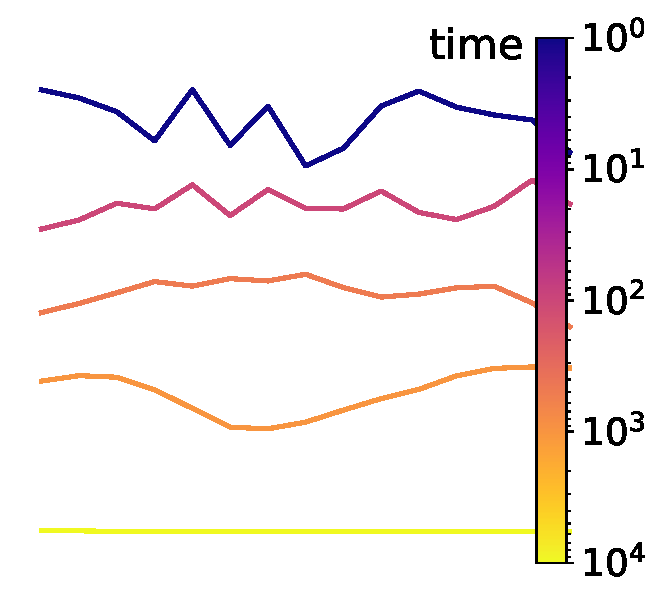
\includegraphics[width=\textwidth]{chain_wave_coarseningN15.pdf} 
       \caption{}
       \label{fig:chain_wc_15}
    \end{subfigure}
    \begin{subfigure}{0.48\textwidth}
       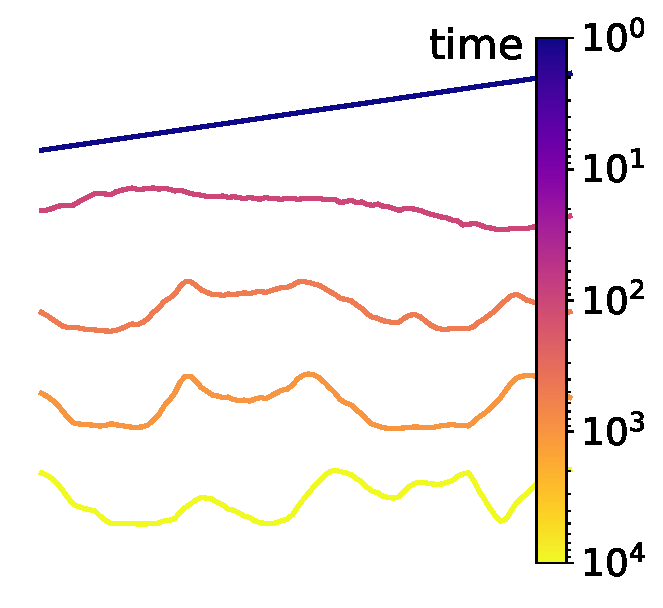
\includegraphics[width=\textwidth]{chain_wave_coarsening_N100.pdf} 
       \caption{}
       \label{fig:chain_wc_100}
    \end{subfigure}
    \caption{\textbf{Wave coarsening in a chain with of non-reciprocal units.}
    The displacement of one side of the chain is shown in the vertical direction as time evolves. 
    \textbf{\ref{fig:chain_wc_15}} Chain of 15 units with random initial conditions. 
    \textbf{\ref{fig:chain_wc_15}} Chain of 100 units with a constant slope as initial condition, which corresponds to a 
    kink in the phase. 
    }
    \label{chain_wave_coarsening}
\end{figure}

We considered several chains with different number of units. For chains with 15 units, we observed synchronization 
after roughly \SI{10e3}{s}, like figure \ref{fig:chain_wc_15} shows. But when increasing the system size to 100 units, 
we observed no synchronization. The reason is that the synchronization timescale \eqref{eq:sync_timescale} scales with the 
square of the system size. Thus, it takes a factor $\left(\frac{100}{15}\right)^2\approx 44$ times longer for the 
100-unit chain to synchronize compared to the 15-unit chain. We verified roughly the scaling by considering chains 
with 10 and 20 units. The synchronization timescale was roughly four times larger.   

We included disorder by considering gaussian distributed contributions to a base value. The amount of disorder was set by 
choosing a specific value of the standard deviation of the Gaussian distribution, for different parameters. 
For low disorder, we observe synchronization. 
If one increases the disorder in the activity parameter, while keeping the neighbour coupling relatively low, 
then one observes several separated regions of synchronization. The units with lowest activity oscillate with small 
amplitude and their phase is appreciably delayed with respect to their neighbours with higher activity, 
although they remain synchronized. As the activity disorder keeps increasing, 
the regions of synchronization become smaller, and some regions are made up of a single unit. 


\begin{figure}
    \begin{subfigure}{0.48\textwidth}
        \begin{tikzpicture}
            \begin{axis}[
        ylabel=Frequency (\si{Hz}),
        xlabel=Chain position,
    ]
        \addplot table [x expr=\coordindex,y index=0] {nat_low_disorder.txt};
    \end{axis}
        \end{tikzpicture}
        \caption{}
        \label{fig:chain_disorder1}
    \end{subfigure}
    \hfill
    \begin{subfigure}{0.48\textwidth}
        \begin{tikzpicture}
    \begin{axis}[
        ylabel=Frequency (\si{Hz}),
        xlabel=Chain position,
    ]
        \addplot table [x expr=\coordindex,y index=0] {nat_high_disorder.txt};
    \end{axis}
\end{tikzpicture}
    \caption{}
    \label{fig:chain_disorder2}
    \end{subfigure}
    \caption{\textbf{Separate synchronization regions in a chain with quenched disorder.}
    The frequency of each unit is shown for two values of disorder in the activity parameter. 
    The disorder is added as gaussian distributed noise with standard deviation $\sigma(k_a)$. 
    \textbf{\ref{fig:chain_disorder1}} The disorder in activity is $\sigma(k_a)=2$. The chain has two synchronization 
    regions. 
    \textbf{\ref{fig:chain_disorder2}} The disorder in activity is $\sigma(k_a)=4$, higher than the previous one. 
    The chain has five synchronization regions. 
    Increasing the disorder yields the breaking of synchronization into smaller regions. 
    The other parameters of the simulation are: $\mu(k_a)=7 \quad k_b=3$.  }
\end{figure}

% \begin{figure}
%     \begin{tikzpicture}
%         \begin{groupplot}[group style={group size=2 by 1}]
%             \nextgroupplot 
%             \addplot table [x expr=\coordindex,y index=0] {nat_low_disorder.txt};
%             \nextgroupplot 
%             \addplot table [x expr=\coordindex,y index=0] {nat_high_disorder.txt};
%         \end{groupplot}
%     \end{tikzpicture}
% \end{figure}

% \begin{figure}[htbp]
%     \centering
%     \begin{tikzpicture}
%         \begin{groupplot}[
%             group style={
%                 group size=2 by 1,
%                 horizontal sep=1.5cm,
%             },
%             width=0.45\textwidth,
%             height=0.35\textwidth,
%             xlabel={Chain position},
%             ylabel={Frequency (H)},
%             title style={font=\small},
%             label style={font=\small},
%             tick label style={font=\footnotesize},
%         ]
%             % Panel 1: low disorder
%             \nextgroupplot[title={(a) title}]
%             \addplot table [x expr=\coordindex, y index=0] {nat_low_disorder.txt};

%             % Panel 2: high disorder
%             \nextgroupplot[title={(b) title}]
%             \addplot table [x expr=\coordindex, y index=0] {nat_high_disorder.txt};

%         \end{groupplot}
%     \end{tikzpicture}
%     \caption{Main caption.}
%     \label{fig:label}
% \end{figure}

\section{Cross cell}
\label{section:cross}

So far we have studied and understood the dynamics of a single active unit and the interactions between two active units in different configurations.
Before analysing the whole 2D Lieb lattice, we thought it would be wise to study the dynamics of a cross or diamond cell. 
The cross cell is made out of four active units and one passive unit, shown in figures \ref{diagram_cross_altermagnet}
and \ref{diagram_cross_ferromagnet}. The passive unit lies in the center of the cross, and 
it is connected up, down, left and right to the four active units. We expect the active units to carry out limit cycles. 
The interaction between the active units is mediated by the passive unit. In some sense, it is like the altermagnet or ferromagnet unit 
cell, but with four active units instead of two. The main difference with the unit cell configurations is the passive site is mediating 
several interactions at the same time. We wondered if the passive unit could synchronize all the active units, if it could synchronize 
only a subset of the active units, or if it wasn't able to synchronize them. 
As we did before, we can consider two differen configurations depending on the sign of the chiralities: ferromagnet and altermagnet. 

\subsection{Ferromagnet cross cell}

The ferromagnet cross cell (figure \ref{diagram_cross_ferromagnet}) 
is made out of four active units with the same chirality, and one passive unit in the center. 
Using the observations made in the previous sections, we expect the four active units to synchronize to the same frequency, and 
oscillate in phase. In order to observe it, we tuned the activity parameters of the units so that they would have similar natural frequencies. 
However, the experimental results shown in figure \ref{fig:ferro_cross_experiments} do not support synchronization. 
We carried out three experimental runs with the same exact activity parameters, and found different results. 
Figure \ref{fig:ferro_cross_experiments} shows the phase difference with respect to the Left unit, as time evolves.
In the first experimental run, the units Left, Center and Right are synchronized, with some occasional phase slips. 
Meanwhile Up and Down have their own frequencies. 
In the second run, up and down move like in the first run. 
The right unit seems to have stopped oscillating. And the center site follows the oscillations of the left one. 
In the third run, up unit is synchronized with the left unit, though there is a big phase slip. The down and right units 
oscillate with independent frequencies. The center site evolves erratically. 
We can take away some conclusions. First, the experimental setup is heterogeneous in the actuators, which we already had noticed  
in other experiments. Second, achieving synchronization in the ferromagnet cross cell is more difficult than expected. The system 
is not very robust under disorder. Third, the system is chaotic. The three experimental runs do not show a unique steady state. 
This could be due to the way the experiment is initiated, which is poking the system with the hand. These leads to different 
initial conditions in the experimental runs. Apparently, the system is sentitive to them.

\begin{figure}[hbtp]
  \begin{center}
      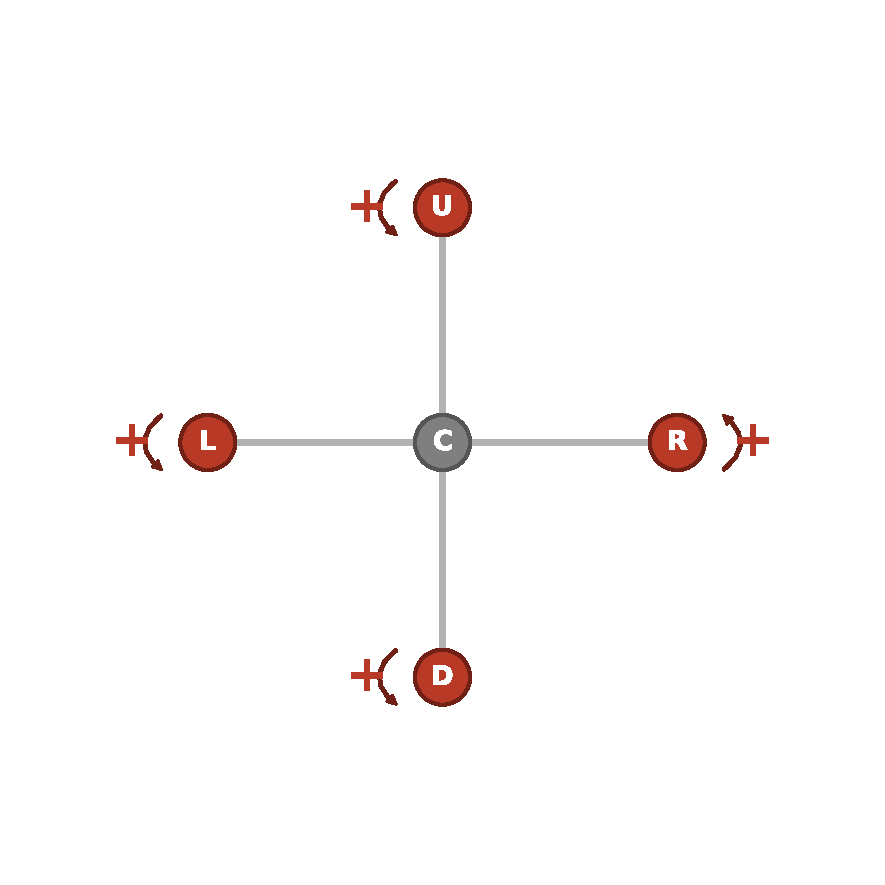
\includegraphics[width=0.3\linewidth]{diagram_ferromagnet_cross_cell.pdf}
  \caption{\textbf{Diagram of the ferromagnet cross cell.}
  The system is made up of four active units with the same chirality connected to a passive site in the center through 
  viscoelastic bands. The cell is a small fragment of a ferromagnetic lattice.}
  \label{diagram_cross_ferromagnet}
  \end{center}
  % Make the graphic take up 90% of the wrapped box
\end{figure}

In simulations, we observed that the system was chaotic. 
In the simple configuration of absolutely identical units, the system synchronizes. 
Moreover, the phenomenom is robust under small disorder in the parameters of the units. 
If one specific parameter of an individual unit is perturbed more significantly, 
for example by an order of 30\% in activity, that particular unit desynchronizes from the rest. 
It can also happen that changing the parameter of one of the units also desynchronizes another unit. 
There is no special preference for which is the other unit that desynchronizes. 
It can be any of the other three active units. The choice is given by the unit whose parameters 
are less similar to the rest (to average of the rest). 
If the units are clustered in pairs in the parameter space, so that two units are similar to each other but quite different to 
the other two, then there are pairs of synchronization. Nevertheless, there is no overall synchronization. 
Interestengly, the passive unit synchronizes with the active units whose frequency is larger, 
although the detuning compared to the passive site's natural frequency (\SI{0}{Hz}) is larger than the detuning of the other active units.
We think that the reason is that the frequency is determined by the activity, but the activity in turn also affects 
the amplitude. As we have seen in other sections, the amplitude has an effect on the Kuramoto coupling. 

\begin{figure}
    \begin{center}
        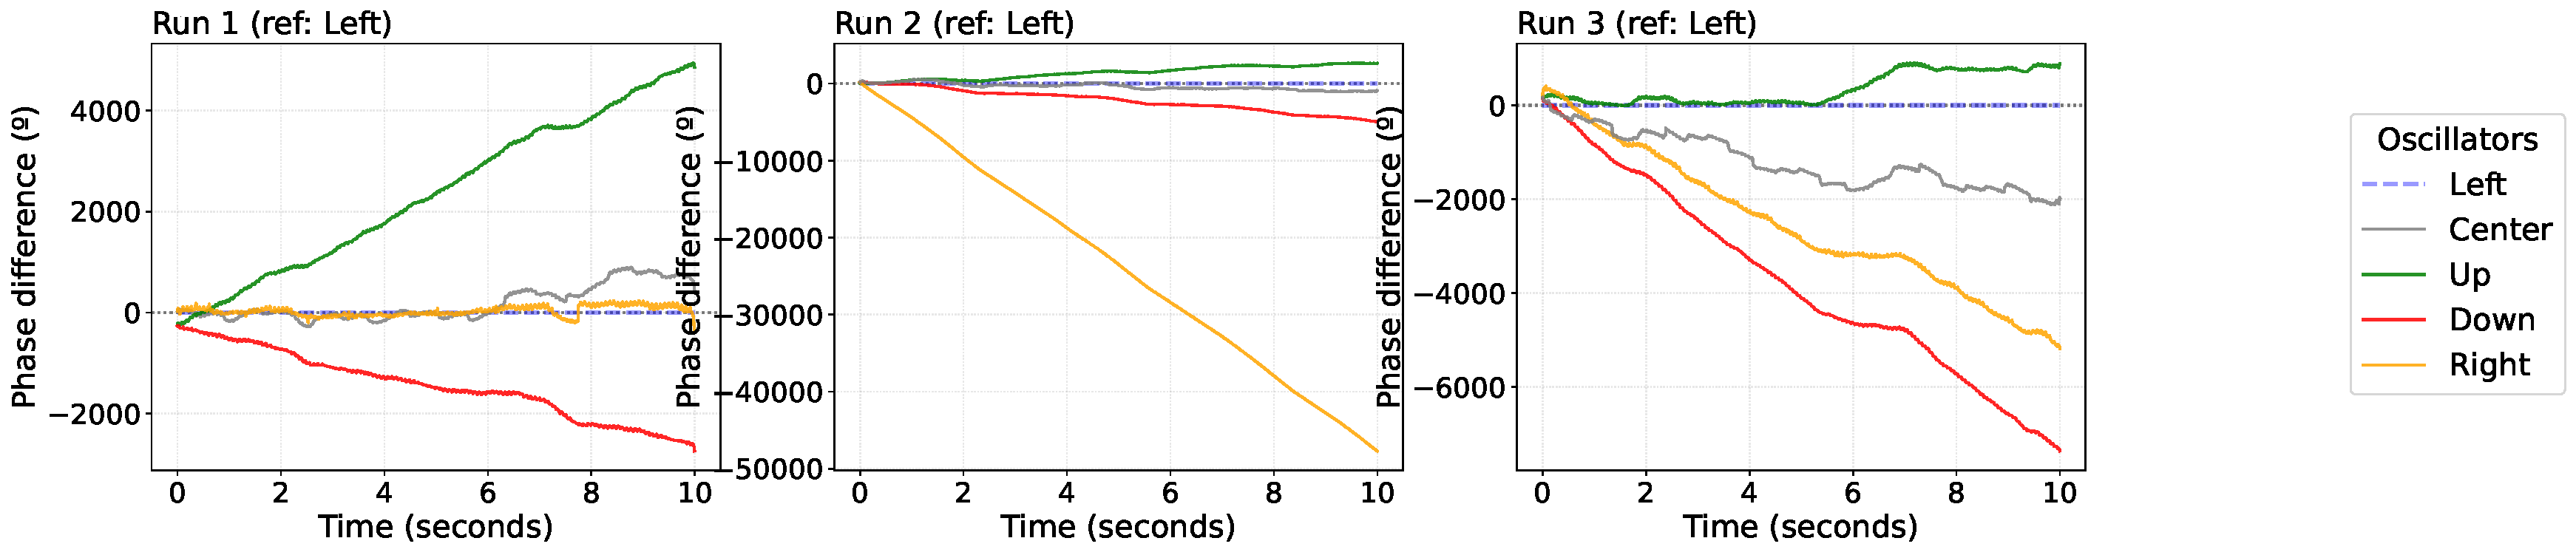
\includegraphics[width=\textwidth]{ferro_cross_cell_exp.pdf}
    \end{center}
    \caption{\textbf{Experimental data of ferromagnet cross cell.} 
    The phase difference with respect to a reference (left unit) is plotted as time evolves for each unit. 
    The different panels correspond to three experimental runs with the same parameter configuration. }
    \label{fig:ferro_cross_experiments}
\end{figure}

\begin{figure}[htbp]
  \centering
  \begin{subfigure}[b]{0.48\textwidth}
    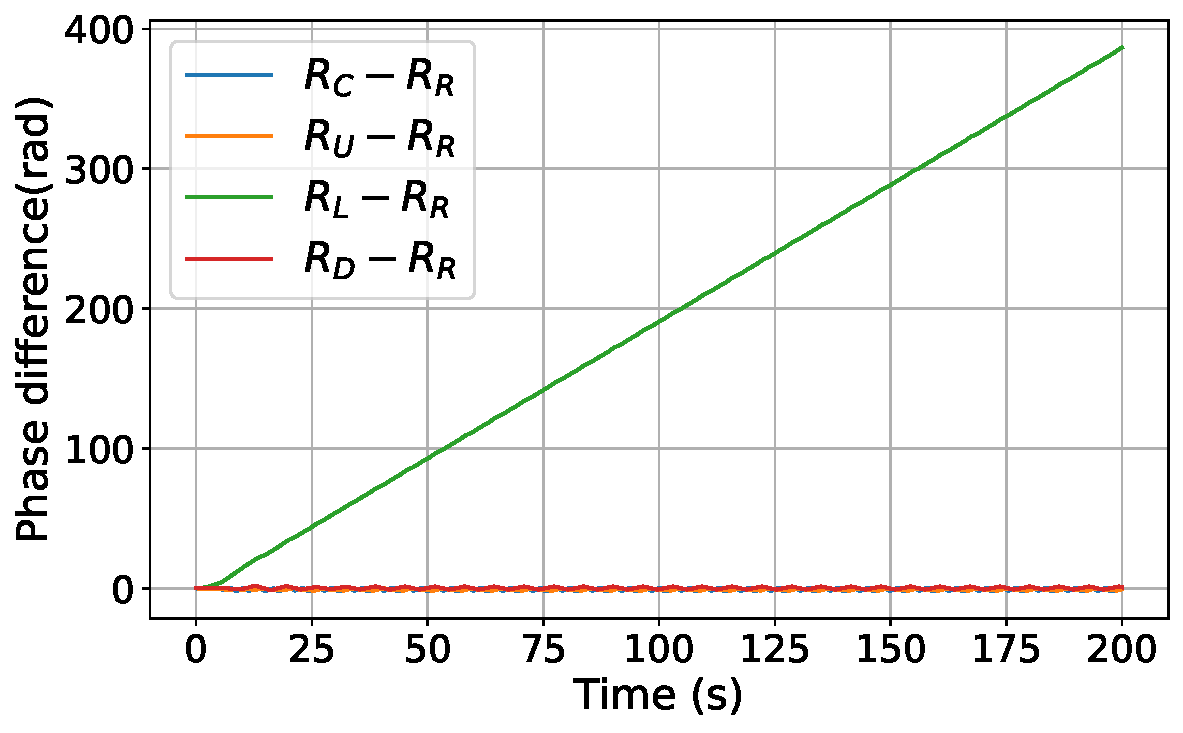
\includegraphics[width=\textwidth]{cross_original_sync_phase.pdf}
    \caption{}
    \label{fig:cross_original_sync}
  \end{subfigure}
  \hfill
  \begin{subfigure}[b]{0.48\textwidth}
    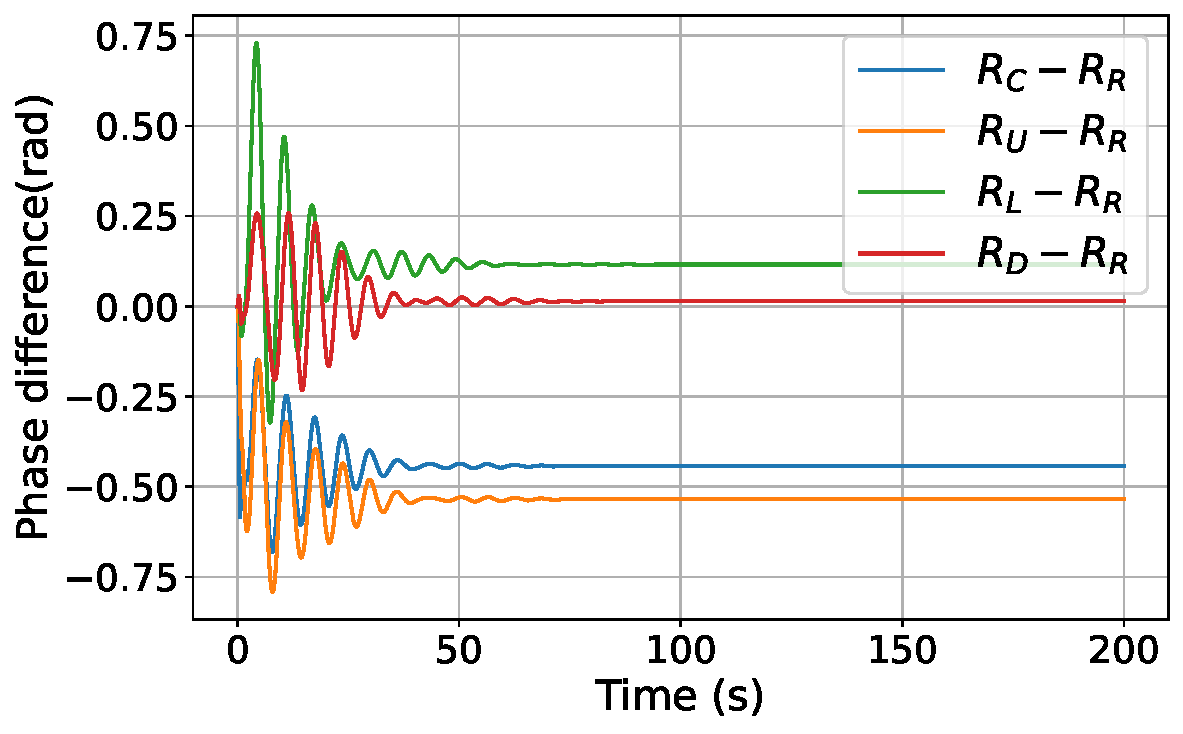
\includegraphics[width=\textwidth]{cross_sync_phase.pdf}
    \caption{}
    \label{fig:cross_sync}
  \end{subfigure}
  \vfill
    \begin{subfigure}[b]{0.48\textwidth}
    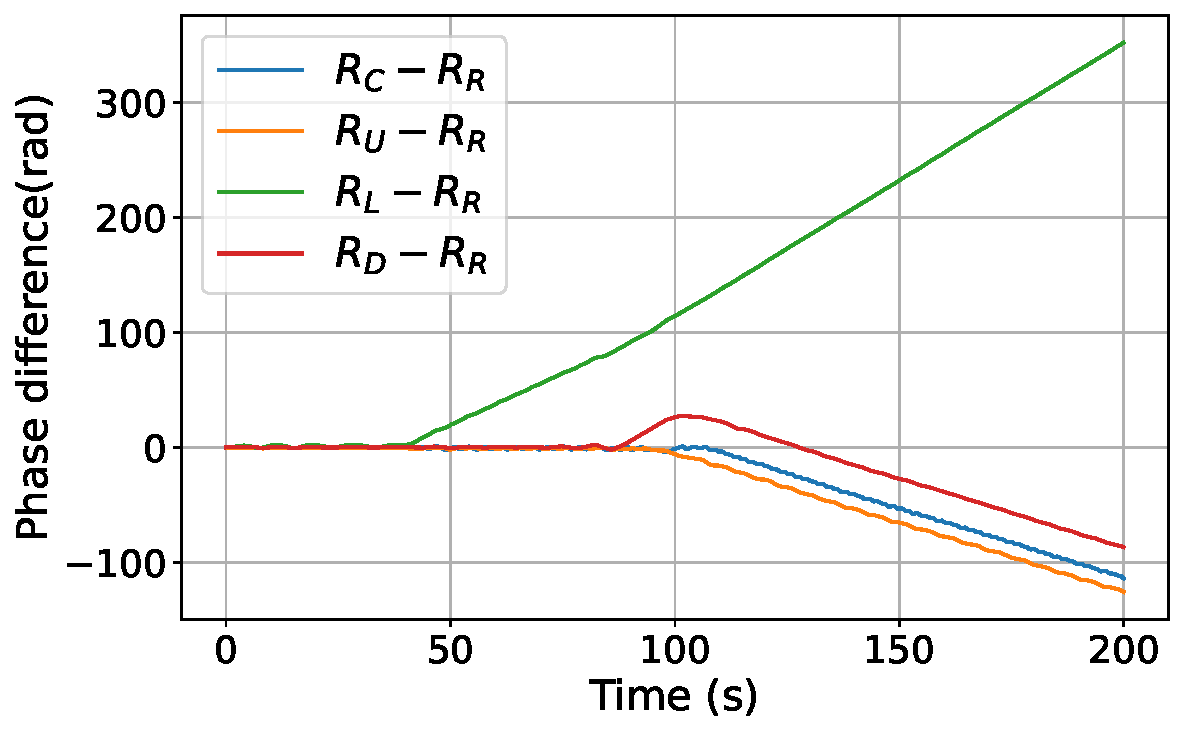
\includegraphics[width=\textwidth]{cross_nosync_phase.pdf}
    \caption{}
    \label{fig:cross_nosync}
  \end{subfigure}
  \hfill
  \begin{subfigure}[b]{0.48\textwidth}
    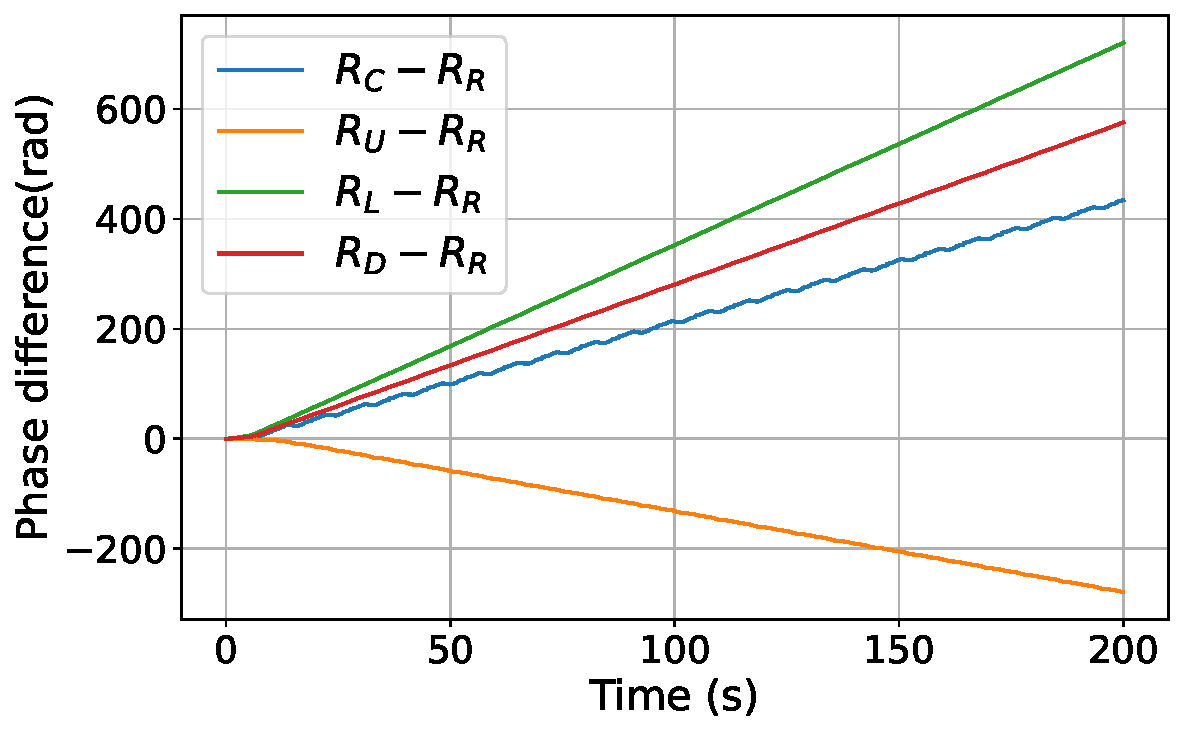
\includegraphics[width=\textwidth]{cross_nosync_atall_phase.pdf}
    \caption{}
    \label{fig:cross_nosync_atall}
  \end{subfigure}
  \caption{\textbf{Simulation data of the ferromagnet cross cell.} 
  Each of the panels has a different behaviour. The parameters of the simulation are damping $\gamma$, onsite stiffness $k_0$, 
  nonlinear cubic saturation $k_c$, activity $k_a$ and elastic coupling of the band $k_b$. The order in which the parameters 
  of each unit are displayed is [Center, Up, Left, Down, Right].
  \textbf{\ref{fig:cross_original_sync}} The left unit is drifting with respect to the rest, which are synchronized. 
    $\gamma = [1, 1.3, 1.17, 1.15, 1.13],\; k_0 = [1.0,  2.0,  1.5,  2.0,  3.0],\;  k_c = 10.0,\; 
    k_a    =  [0, 6, 10, 8, 7],\;  k_b = [6.0, 4.0, 5.0, 3.0]$.
  \textbf{\ref{fig:cross_sync}} All the units synchronize. The only change compared to the parameters of \ref{fig:cross_original_sync} 
  is the activity of the left unit $k_a =  [0, 6, 10, 8, 7]$.
  \textbf{\ref{fig:cross_nosync}} The up, down and center units remain synchronized. The left and right units have their own frequency. 
  The only parameter change with respec to \ref{fig:cross_original_sync} is the elastic neighbour band coupling 
  of the left unit $k_b = [6.0, 5.0, 5.0, 3.0]$. Modifying the parameters of the left unit stops the synchronization of the right unit. 
  \textbf{\ref{fig:cross_nosync_atall}} No synchronization between any of the units. They all oscillate with different frequency.
  In order to achieve it, the disorder is increased. 
    $\gamma = [1, 1.3, 1.7, 1.5, 1.3],\; k_0 = [1.0,  2.0,  1.5,  2.0,  3.0],\; k_c  = 10.0,\; 
    k_a    =  [0, 5, 15, 12, 7],\; k_b = [6.0, 6.0, 5.0, 3.0]$.  
  }
  \label{fig:cross_cell_ferro}
\end{figure}
%%%%%%%%%%%%%%%%%%%% wrong
% In those cases, we observed that the other unit was the one on the opposite side 
% to the perturbed one. This scenario corresponds to a whole row synchronized, 
% either vertical or horizontal, and the two perpendicular units desynchronized.
% Therefore, the passive site is only mediating the synchronization between 
% the two active units with the same chirality.
For all units to oscillate with different frequencies, 
one must make the different perturbations for every unit, which leads to huge differences 
in the parameters. The same example of perturbing the activity requires differences 
of more than 100\% between some of the units. This shows that synchronization is indeed robust. 
One can always recover synchronization by increasing the neighbour coupling of the specific units
that are greatly perturbed. This observation agrees with the conclusions derived from the 
Adler equation \eqref{eq:adler}. Notice however, that the Adler equation only takes into 
account mismatches in the natural frequency. The simulations show that an analogous phenomenom 
happens for mismatches in other parameters, like activity or damping. 

\begin{figure}[htbp]
  \centering
  \begin{subfigure}[b]{0.48\textwidth}
    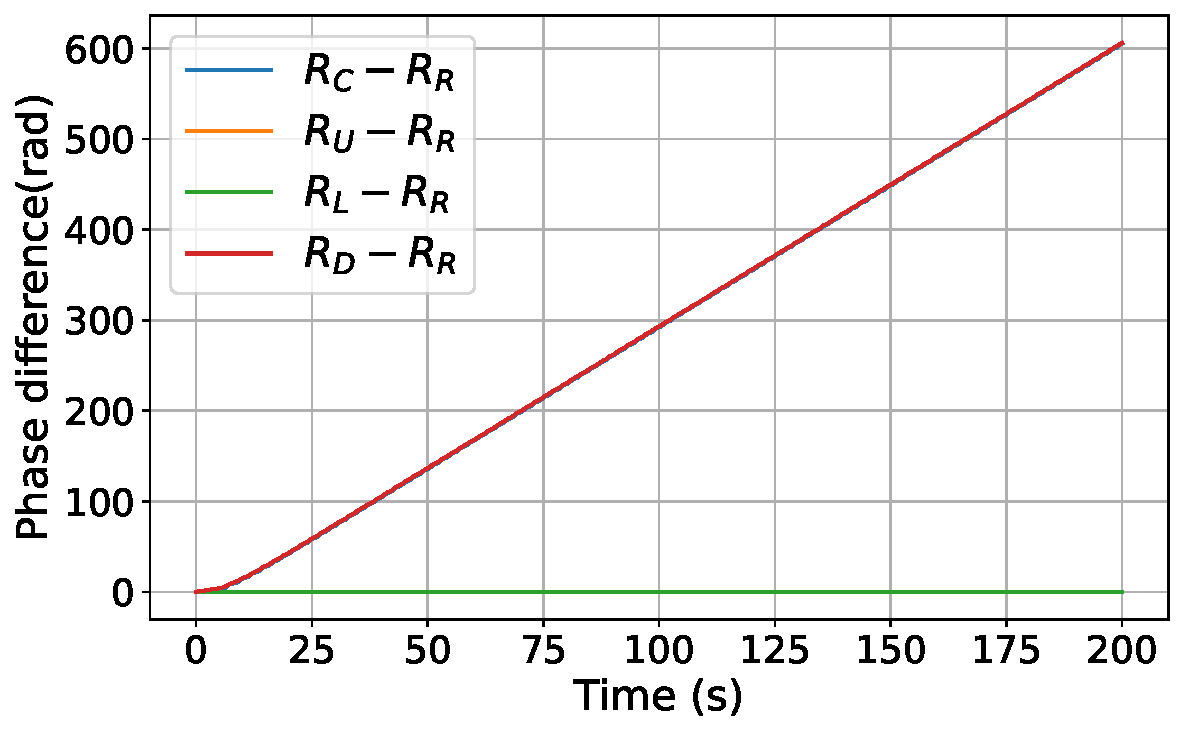
\includegraphics[width=\textwidth]{cross_UD_phase.pdf}
    \caption{}
    \label{fig:crossUD}
  \end{subfigure}
  \hfill
  \begin{subfigure}[b]{0.48\textwidth}
    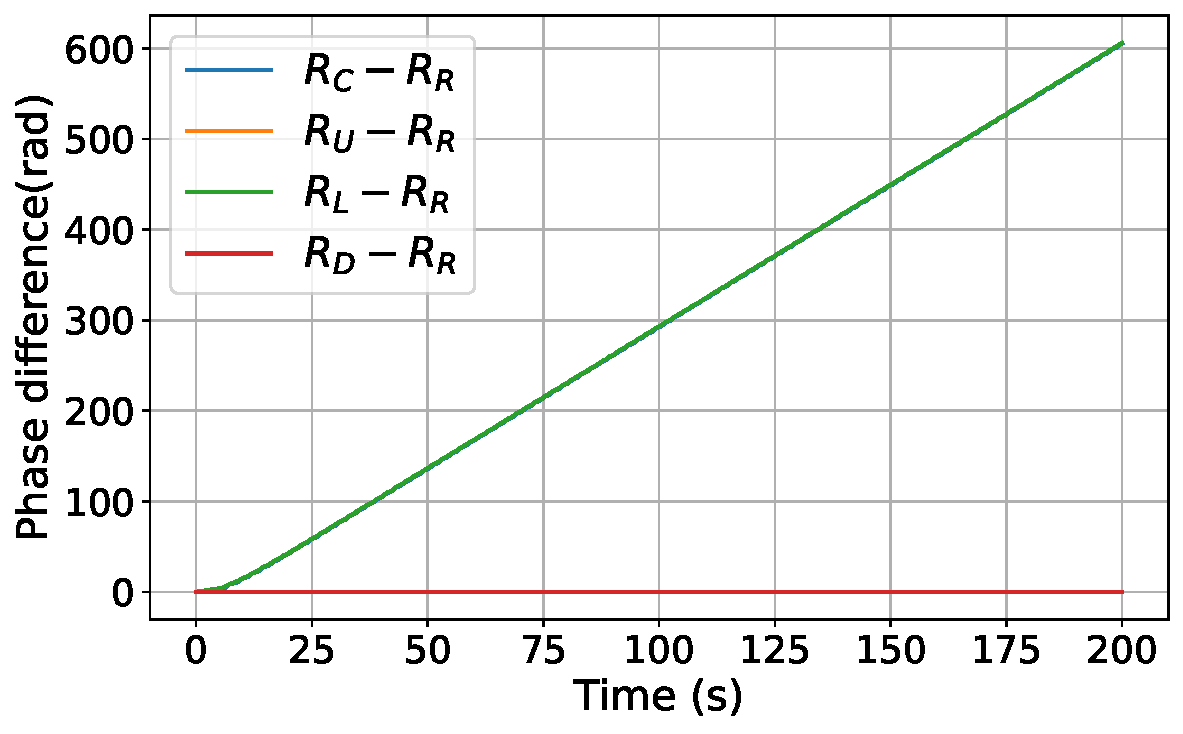
\includegraphics[width=\textwidth]{cross_UL_phase.pdf}
    \caption{}
    \label{fig:crossUL}
  \end{subfigure}
  \caption{\textbf{Symmetric configurations in pairwise synchronization of ferromagnet cross cell.}
  The plots show the equivalence of the two possible pairwise synchronization configurations. 
  \textbf{\ref{fig:crossUD}} Synchronization Up-Down and Left-Right.
  \textbf{\ref{fig:crossUL}} Synchronization Up-Left and Down-Right.
  }
  \label{fig:cross_cell_identical}
\end{figure}

\subsection{Altermagnet cross cell}

The altermagnet cross cell (figure \ref{diagram_cross_altermagnet}) 
is made out of one passive unit in the center, two active units above (up) and below (down) the passive one with the same chirality, 
and two active units on the left and right of the passive one with opposite chirality.

\begin{figure}[hbtp]
  \begin{center}
      % Make the graphic take up 90% of the wrapped box
  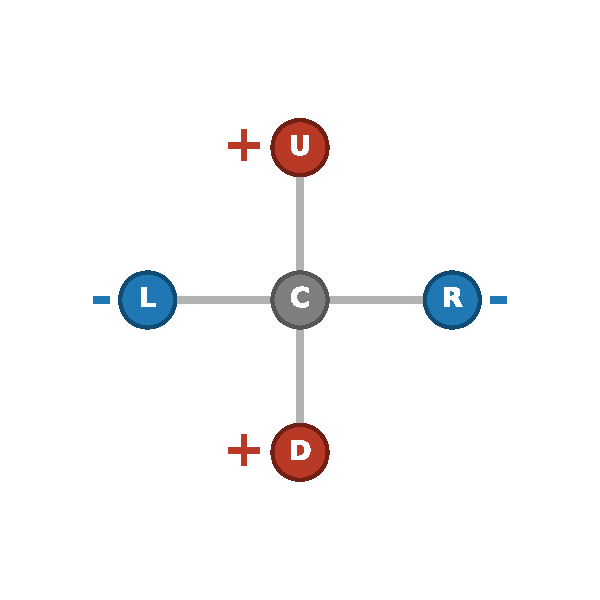
\includegraphics[width=0.4\linewidth]{diagram_am_cross_cell.pdf}
  \caption{\textbf{Diagram of the altermagnet cross cell.} 
  There are four active units connected to a passive central one through viscoelastic bands. 
  Up and down units have positive chirality, while left and right units have negative chirality. 
  The cell is a small fragment of the altermagnetic Lieb lattice. }
  \label{diagram_cross_altermagnet}
  \end{center}
\end{figure}

Figure \ref{am_cross_cell_phase} shows the phase of each of the units in time, for different experimental runs.
First, focus on the up and down units, which increase with a constant slope. Note that the down unit, depicted with orange line, 
is overlapped with the red line. This means that these two units are completely synchronized. This is the case in both 
experimental runs. Focusing on the first run, there are also two units, right and left, whose phase decreases in time.
These units don't have the same phase, as we see that the lines separate with time. Hence, they are not synchronized. 
In comparison, on the plot on the right, the lines coincide for most of the experiment. At the end, it seems like they separate. 
The reason they separate is a phase slip. Phase slips are brief moments where the oscillators go out of sync before 
going back again into in-phase synchronization. %[explain in intro?]. 
Note that after the phase slip, the slope of both lines remains the same, meaning that their frequency is the same. So they 
synchronize again. The difference in experimental parameters between the two plots in \ref{am_cross_cell_phase} 
is the activity of the left and right units. For the plot on the left, $k_a^L = -4 = k_a^R$, while for the plot 
on the right $k_a^L = -7 = k_a^R$. Therefore, increasing the activity leads to better chances of synchronization. 
We already stated the same conclusion in the previous section.

\begin{figure}[hbtp]
    \begin{center}
        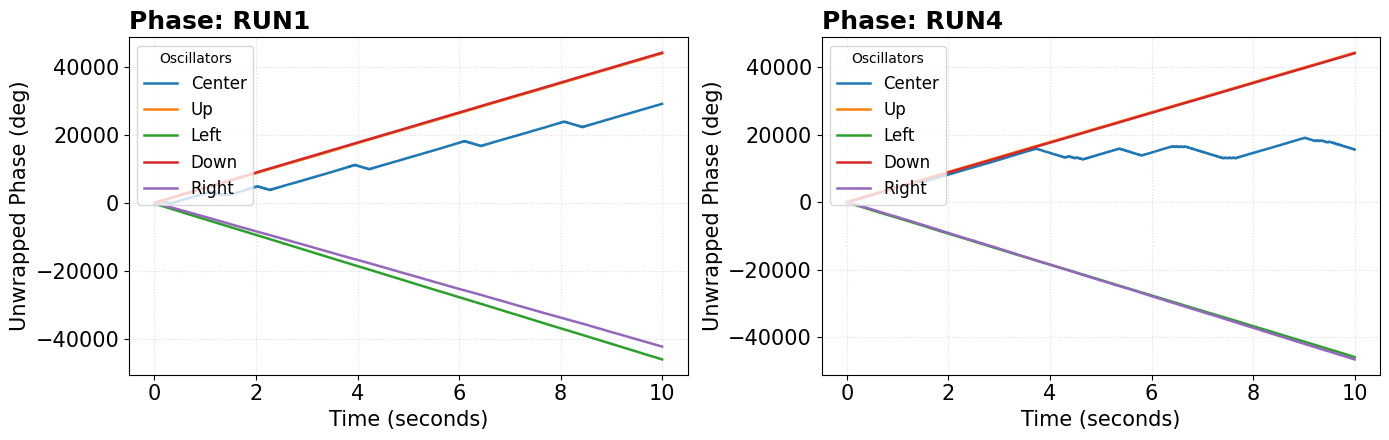
\includegraphics[width = 0.8\textwidth]{am_cross_cell_phase.png}
        %\captionsetup{justification=justified}
        \caption{\textbf{Experimental data of altermagnet cross cell.}
        The phase of each unit is shown as time evolves.
        \textbf{Run 1:} The active units have the same absolute value of activity: $k_a^U = 4 = k_a^D$,  $k_a^L = -4 = k_a^R$.
        Up and down units have their lines overlapped, which means they are synchronized. The left and right lines do not overlap, so 
        they are not synchronized. This is because the passive site has a tendency to synchronize with the up and down units, 
        since the slope is most of the time parallel to those units' lines. The passive site is responsible for the interactions leading 
        to the synchronization of the positive-chirality units, and also for the drifting of the negative-chirality units. 
        Such a tendency to synchronize with the up and down units is explained by the action of gravity in the vertical direction. 
        Gravity pulls on the viscoelastic band, increasing its tension. This results in a slightly stronger coupling in the vertical 
        direction compared to the horizontal direction. The band array is not fixed to the sides of the apparatus.
        \textbf{Run 4:} $k_a^U = 4 = k_a^D$,  $k_a^L = -7 = k_a^R$ The activity of the negative-chirality units is increased in comparison 
        with the previous experimental run. The notable effects are the synchronization of those units, the left and right ones. 
        Moreover, the passive site's motion is more evenly distributed between the two stable states. Increasing the 
        activity of the negative-chirality units seems to compensate for the asymmetry generated by gravity. }
        \label{am_cross_cell_phase}
    \end{center}
\end{figure}

There is a fifth unit, the passive one in the center, and it is actually the most interesting one in this system 
because it mediates the interactions between the active ones. %We are very interested in its mtoion. 
Its phase exhibits step-like motion: there are straight lines and vertices where the slope of the straight line changes abruptly. 
An important feature is that the slope of the phase is either the same as the up and down units, or the same as the left and right units. 
Therefore, the center passive unit is sometimes synchronizing with the positive chirality active units and other times with the 
negative chirality units. It seems to be alternating between both scenarios. The system is therefore bistable, and it jumps from 
one stable state to the other. However, the unit is frustrated because it cannot 
synchronize with both of the chiralities at the same time. One thing to keep in mind is that the passive unit 
is not tracing out a clear limit cycle like the active units. Its motion in phase space is more messy. Still, one can change from 
the displacement coordinates of both actuators to polar coordinates $(x_1,x_2)\longrightarrow (R,\phi)$ and study its phase. 

A priori, the center unit can choose any of the active units to synchronize itself with. Nevertheless, 
figure \ref{am_cross_cell_phase} and other experiments show a tendency to synchronize with the up and down units more 
often than with the left and right units. Here, we go back to the discussion we had in the previous section about 
horizontal and vertical couplings, and the slight difference in results between them. The general tendency of synchronizing 
with the up and down units is an indicator of the asymmetry between the vertical and horizontal coupling. From the results, 
one estimates that the vertical coupling, the one connecting the center node to up and down, is stronger than the horizontal coupling. 
The reason for the asymmetry is that gravity is acting on the vertical direction. Thus, the viscoelastic band is stretched and under more 
tension, making the effective elastic stiffness slightly stronger. Note that the viscoelastic band is fixed to the structure at the top, so 
that it doesn't fall, while it is not fixed to the sides. We think this is the reason for any asymmetry in the coupling directions 
and specifically, for the tendency of the center node to synchronize with its vertical neighbours. 

%[add simulation reults and discussion comparison]
%%%%%%%%%%%%%%%%%%%%%%%%%%%%%%%% simulations
We contrasted the experimental results with simulations of the altermagnet cross cell. For completely identical units, 
we obtained that the passive site alternates evenly between positive and negative chirality, as shown in figure \ref{fig:cross_am_sym}.
In this case, the same chirality units are synchronized. So Up and Down units are synchronized to a positive frequency, 
while the Left and Right units are synchronized to a negative frequency. However, by introducing a small disorder in the 
damping, the active units of same chirality do not synchronize. The results are depicted in figure \ref{fig:cross_am_damping}. 
Moreover, the motion of the passive unit becomes very 
erratic. There is no noise added to the system, so the simulation is deterministic. The changes in the frequency of the 
passive unit are due to chaotic behaviour. 
\begin{figure}[htbp]
  \centering
  \begin{subfigure}[b]{0.48\textwidth}
    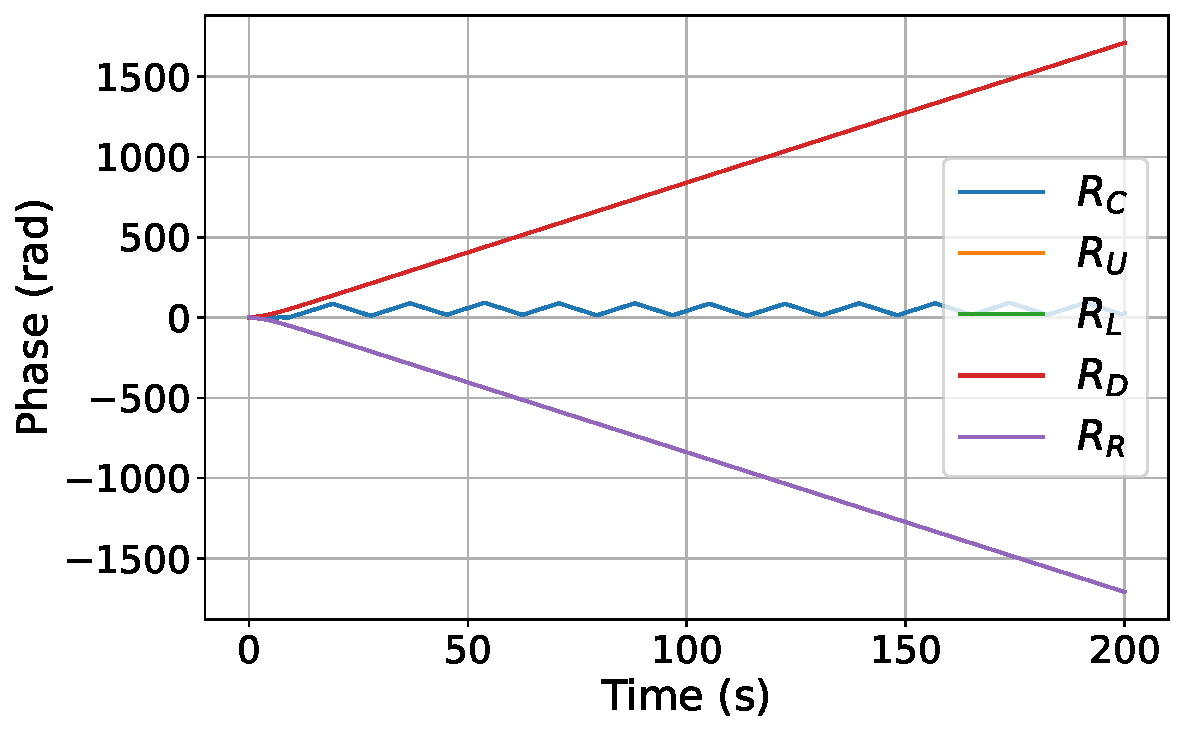
\includegraphics[width=\textwidth]{cross_altermagnet_symmetric_phase.pdf}
    \caption{}
    \label{fig:cross_am_sym}
  \end{subfigure}
  \hfill
  \begin{subfigure}[b]{0.48\textwidth}
    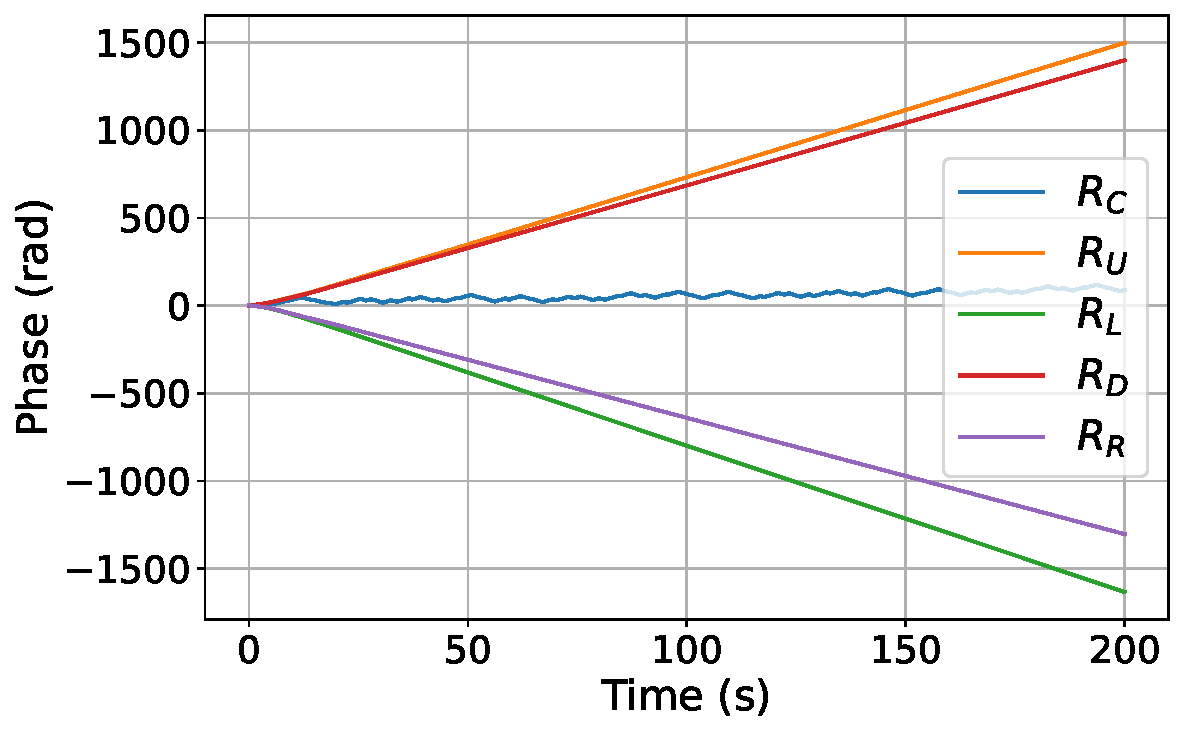
\includegraphics[width=\textwidth]{cross_altermagnet_damping_disorder_phase.pdf}
    \caption{}
    \label{fig:cross_am_damping}
  \end{subfigure}
  \caption{\textbf{Simulation data of altermagnetic cross cell, with and without disorder.}
  The phase of each unit is shown as time evolves. 
  The parameters of the simulation: $k_0 = 2 \quad k_c = 10 \quad k_a = 10 \quad k_b = 3$. 
  \textbf{\ref{fig:cross_am_sym}} Simulation with no disorder: $\gamma=1$ for all units. Units with same chirality synchronize. 
  The passive unit alternates evenly between synchronization with positive and negative chiralities, yielding a seesaw line. 
  \textbf{\ref{fig:cross_am_damping}} Simulation with quenched disorder in the damping: $\gamma = (1.1, 1.3, 1.2, 1.4, 1.5)$. 
  Units with the same chirality do not synchronize. The passive unit alternates between bistable states chaotically. 
  }
  \label{fig:cross_am_simulation}
\end{figure}

\section{Bilayer Lieb lattice}
\label{section:lieb}

In order to replace the spin degree of freedom at the sites of a Lieb lattice with mechanical oscillators, 
we need two Lieb-lattice layers of linear actuators. 
As before, pairs of actuators mirrored across the wall interact non-reciprocally. Within each Lieb-lattice layer,
neighbouring actuators are coupled by viscoelastic bands. 

\subsection{Simulations of the overdamped regime}

We wanted to observe if spin-momentum locking was present in the mechanical Lieb lattice. 
This meant observing positive chirality waves propagating in one direction, and negative chirality waves 
in another direction. In order to do so, we had to set the activity to be in the overdamped regime before the 
Hopf bifurcation. In this regime, friction dominates and waves are attenuated. This is a good thing to observe 
spin-momentum locking. The bad thing is that this regime is difficult to access experimentally. Since the waves are attenuated, 
the actuator displacements are very small and cannot be measured. For that reason we resorted to simulations. 

\begin{figure}[htbp]
  \centering
  \begin{subfigure}[b]{0.32\textwidth}
    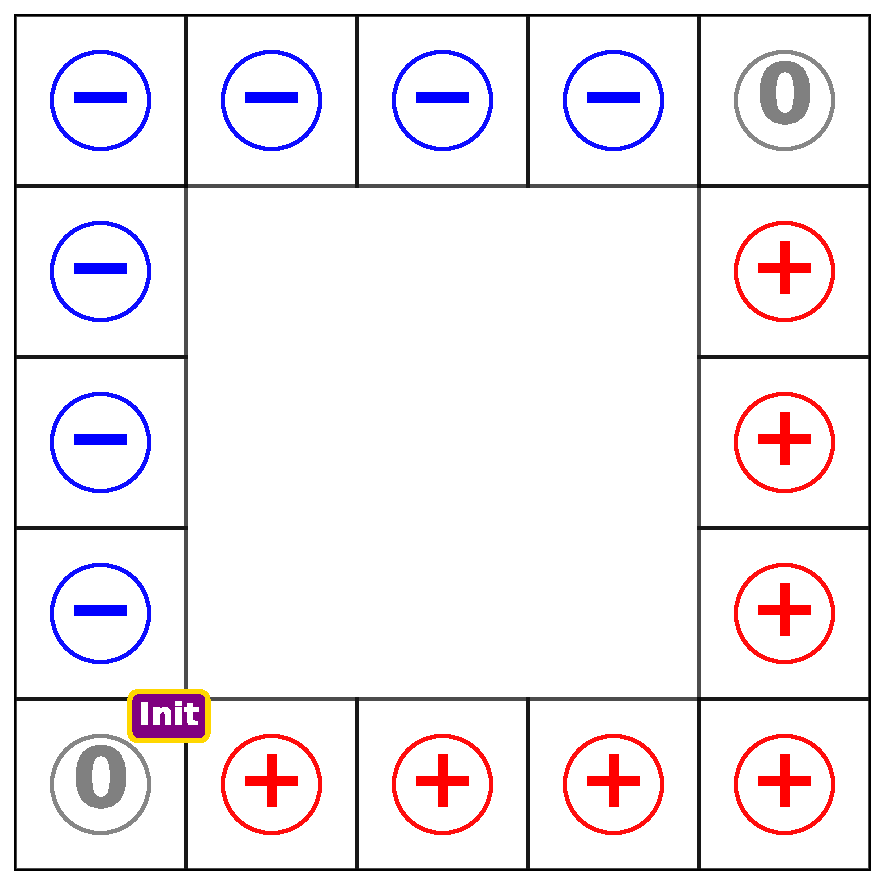
\includegraphics[width=\textwidth]{lieb_sml_gen_compacted.pdf}
    \caption{}
    \label{fig:lieb_sml_gen}
  \end{subfigure}
  \hfill
  \begin{subfigure}[b]{0.32\textwidth}
    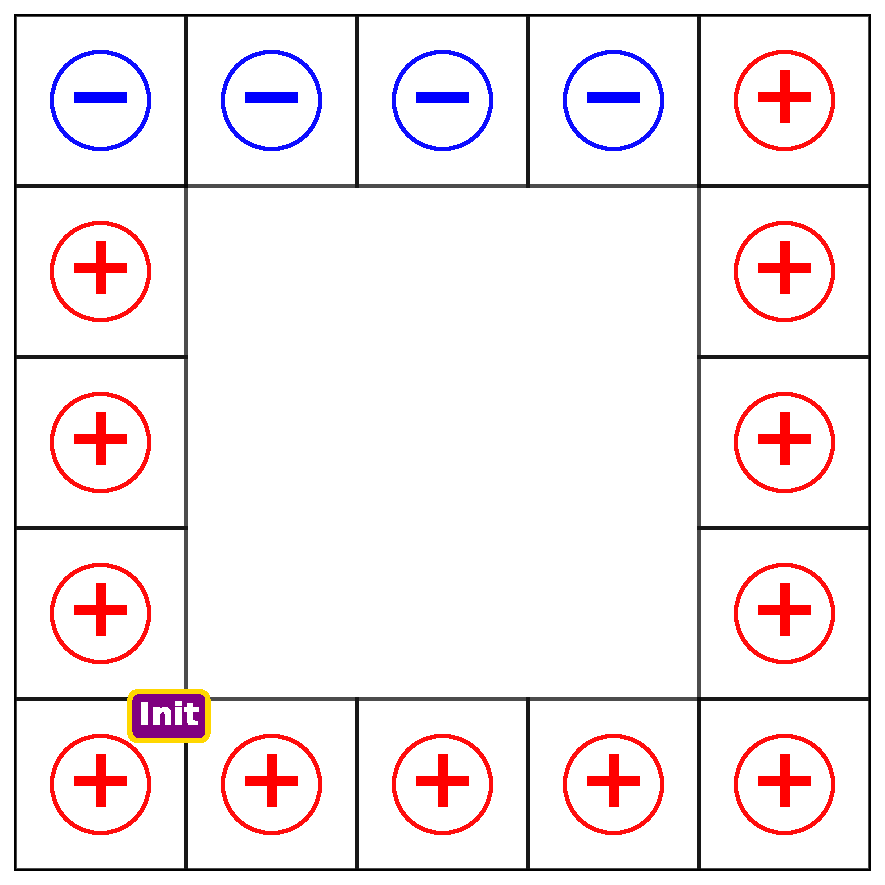
\includegraphics[width=\textwidth]{lieb_sml_pos_compacted.pdf}
    \caption{}
    \label{fig:lieb_sml_pos}
  \end{subfigure}
  \hfill
    \begin{subfigure}[b]{0.32\textwidth}
    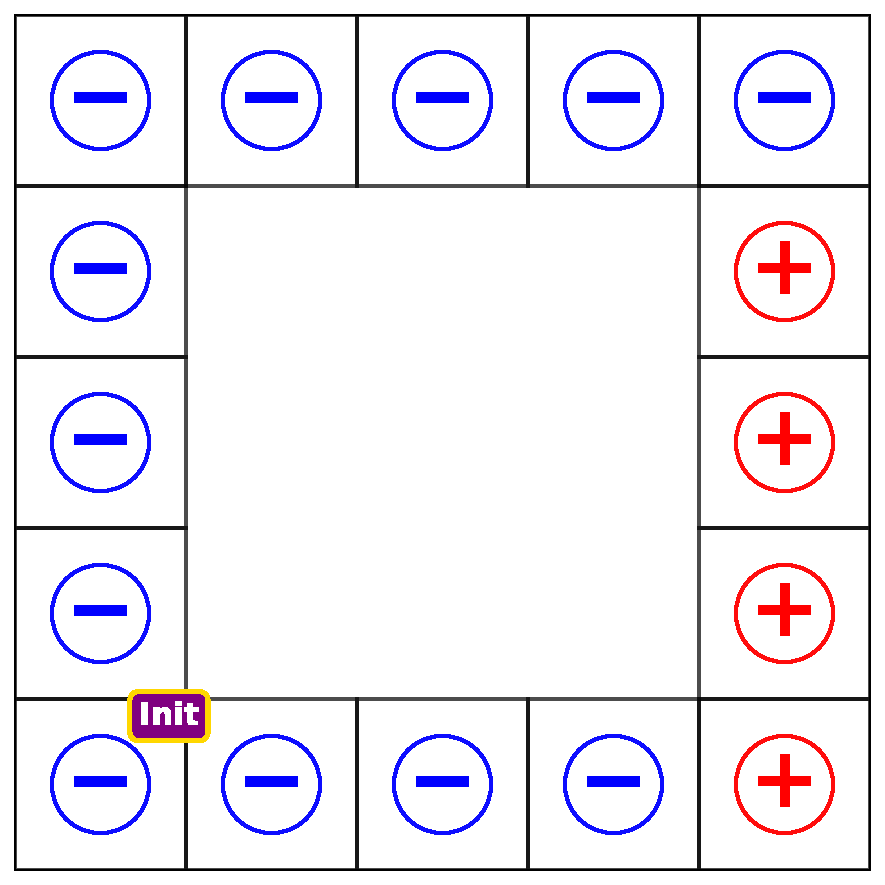
\includegraphics[width=\textwidth]{lieb_sml_neg_compacted.pdf}
    \caption{}
    \label{fig:lieb_sml_neg}
  \end{subfigure}
  \caption{\textbf{Chirality-momentum locking in mechanical Lieb lattice. }
  Diagram illustrating the chirality of the passive sites in the edges of the mechanical Lieb lattice. 
  It is a simulation of the overdamped regime.
  The chirality is measured as the average angular momentum of the unit: $J = x_1 \dot{x}_2 - x_2 \dot{x}_1$.
  The system is perturbed initially on the bottom left corner. We consider three different initial conditions, 
  depending on the chirality of the perturbation.  
  \textbf{\ref{fig:lieb_sml_gen}} The initial perturbation is a kick with no chirality. The positive-chirality component 
  is amplified in the horizontal direction. Thus, the bottom and right edges have positive chirality. The negative-chirality 
  component is amplified in the vertical direction. Hence, the left and top edges have negative chirality. 
  \textbf{\ref{fig:lieb_sml_pos}} Although the initial perturbation has positive chirality, the top edge remains with negative chirality. 
  \textbf{\ref{fig:lieb_sml_neg}} Although the initial perturbation has negative chirality, the right edge remains with negative chirality. 
  The property of chirality-momentum locking is independent of the initial perturbation.
  }
  \label{fig:lieb_sml}
\end{figure}

The simulation consists of a 9x9 Lieb lattice of non-reciprocal units. The initial condition is a perturbation in the 
lower left corner of the lattice. We observe the waves that propagate thorugh the system. Since friction dominates, 
they eventually die out. The motion of the active units is constrained by their built-in chirality. Nevertheless, 
we can analyse the chirality of the passive sites to know where each chirality propagated. We do so 
by measuring the angular momentum of the passive sites: $J = x_1 \dot{x}_2 - x_2 \dot{x}_1$. 
If $J>0$, it means that the passive site has positive chirality, and if $J<0$, negative chirality. 
For simplicity, we show in figure \ref{fig:lieb_sml} the angular momentum of the passive sites on the edges of the Lieb lattice.
We considered three initial conditions. The first one, figure \ref{fig:lieb_sml_gen}, has a kick as initial condition. 
The kick has no associated chirality, and so it is displayed in the figure as a 0. We observe that the chirality 
of the passive sites to the right is positive, while the chirality of the passive sites towards the top is negative.
As in the case of a magnetic Lieb lattice, the positive chirality component of the perturbation is amplified 
in the horizontal direction. That is why we see the bottom and the right edges with a plus sign. In contrast, the 
negative component is amplified vertically, and we observe the left and top edges with a minus sign. 
This is precisely the same phenomenom of spin-momentum locking oberved in altermagnets. 

In subfigure \ref{fig:lieb_sml_pos}, the initial condition is changed to a positive chirality perturbation. 
The difference is on the left edge, which is now positive due to the initial condition. Nevertheless, we still 
observe that the top edge has negative chirality, even though the perturbation is of positive chirality. 
A similar thing happens in the last panel \ref{fig:lieb_sml_neg}, where the initial conditon is a negative chirality perturbation.
Although the closest passive sites acquire negative chirality, the right edge still displays positive chirality. 

\section{Conclusion}

In conclusion, we implemented oscillator chirality in a metamaterial platform. The original idea behind the implementation was to 
replace the spin angular momentum of magnetic materials. Chirality was achieved by coupling two actuators
non-reciprocally. The actuators performed limit cycles in phase space that behaved like an oscillator. 
It allowed the study of systems of various dimensions and symmetries. Some of those were analogous to 
ferromagnets, antiferromagnets and altermagnets, but in a classical setting. Our main motivation was the study of recently discovered 
altermagnets, which have become a trending topic in condensed matter physics. The motivation made us switch disciplines quickly 
to the fields of nonlinear dynamics, metamaterials and soft matter. The experimental milestone was the construction 
of a Lieb lattice of mechanical actuators. We started by analysing its microscopic properties, which led us to the theory 
of nonlinear oscillators. After that, we analyse the macroscopic behaviour of the system, 
and also explored different geometries and symmetries. The analysis included experimental results, but also 
comparison with theoretical predictions and further investigations using simulations.

Despite the physical actuators being imperfect or defective, we still observed signs of the corresponding scalings 
predicted by the supercritical Hopf bifurcation. This result was a nice sanity check. There were two different regimes, either before 
or after the Hopf bifurcation. Before the bifurcation, friction dominated. The oscillations were attenuated and the system came to rest. 
By increasing the activity parameter, i.e. the energy input, the system underwent the Hopf bifurcation, resulting in the 
formation of limit cycles. The clockwise direction of the limit cycle was associated with negative chirality, and the 
counterclockwise direction with positive chirality. There was a third type of unit without activity, called passive.
We studied both regimes separated by the bifurcation. However, it was difficult to measure experimentally in the overdamped regime. 
In that case, we carried out simulations. 

The next step was the study of pairwise interactions between the oscillatory units. 
We realised that units with the same chirality have a parameter region where they synchronize, 
similarly to other oscillatory systems. However, if the units had opposite chirality, we didn't observe synchronization. 
If passive units were added, they would absorb some energy from the active ones and use it to follow the motion of their neighbours. 
The theoretical models predict that synchronization is caused by the viscous interaction rather than the elastic one. 
This was an interesting result, because the primitive models did not include the viscous term. 
 

Next we studied the one-dimensional chain of units. If the active units had the same chirality, they synchronized with a large amplitude 
in the regime after the Hopf bifurcation. In the regime below the bifurcation, perturbations propagated through the chain with 
small attenuation. If some active unit had opposite chirality, then the perturbations stopped propagating when reaching that 
particular unit. In the limit cycle regime, the oscillation amplitude was significantly reduced. These effects were an 
expression of selective propagation depending on the chirality of the units. 
We studied more complicated features like the transient dynamics and the effect of the system size using simulations. 
The transient dynamics, that takes the chain from the initial condition to the complete synchronization, is governed by 
wave coarsening. In experiments, synchronization happens very fast, indicating a very small synchronization timescale. 
The system size affects such timescale. For longer chains, one needs to wait more time to reach the synchronized steady state. 

The experimental results up to now suggested that a ferromagnetic lattice of oscillators after the Hopf bifurcation would have all 
the units synchronized to a single frequency. For the altermagnetic Lieb lattice, all the positive chirality units would synchronize 
together to some frequency, and all the negative chirality units would synchronize to another frequency. 
However, that is not what we observed when studying small fragments, the cross cells, of those systems. 
The synchronization phenomenom in the ferromagnet cross cell seems to be less robust than expected. The consequence 
is the experimental absence of synchronization. Simulations with small quenched disorder support the claim. 
The altermagnet cross cell is bistable, and its passive unit is frustrated 
between synchronizing with the positive and negative chirality units. The passive unit alternates chaotically between both 
states, even in simulations.  

We simulated the mechanical Lieb lattice in the overdamped regime. The system exhibited chirality-momentum locking, 
like the original magnetic Lieb lattice. This allows the transmission of different signals by means of mechanical waves, in 
perpendicular directions. The signals are filtered nicely so there is no mixing. Nevertheless, these waves are 
significantly attenuated. To overcome this obstacle one would need to decrease the friction of the passive units. 
The friction of the active units can be compensated with activity.  


\newpage

\section*{Acknowledgements}

Thanks to all the people involved in the project. Thanks to Corentin Coulais and Jasper van Wezel for guiding me throughout 
the year, both academically and morally. I am profoundly grateful to Yuan Zhou, Rupesh Mahore and Viktor Könye for their 
inexhaustible efforts in attending requests, answering questions and overcoming obstacles. 

I am immensely indebted to the 
University of Amsterdam's Technology Centre for turning the theoretical dreams into reality. In particular, 
I owe my deepest gratitude to Ronald Hassing for designing and building the experimental platform, as well as for his 
generous endeavour and support. Special thanks to Kasper van Nieuwland for the development of the electronic 
aspect of the system, and his willingness to meet for improvements. On the same note, thanks to Mels van Eck. 

My sincere thanks to everyone in Jasper's group: Esther, Lizzy, Javier, Fran, Shengze and Joseph. I have learned 
a lot from the group meetings and discussions. My special thanks to Jasper for taking the time to explain concepts in depth.
Moreover, thanks to the Machine Metamaterials group for their inspiring figures, ideas and discussions. 
Special thanks to Tianhao, Guus, Lode and Mingyang for the friendly and supportive atmosphere.

I am absolutely grateful to Fundación Mutua Madrileña for the funding of the project.  
Thanks to my friends and family for taking care of me. 

\newpage

\nocite{*}
\printbibliography

\newpage

\begin{appendices}

\section{Calibration of actuators}

We calibrated the properties of the linear actuators with two methods. The first involved poking them and measuring the 
damped oscillations. We fitted the position data to an exponentially attenuated wave: $f=Ae^{-\gamma t}\cos{(\omega t + \phi)}+c$.
The results of the fit are shown in table \ref{tab:node_fit_parameters}. 
The second method was measuring the force-displacement curve on an Instron machine. The curves were measured for a 
single actuator at different rates. The results are shown in figure \ref{fig:instron_actuator_calibration}.
% Further analysis of these curves allows the calculation of the damping coefficient. Its value was dependent on 
% the position and the rate 

\begin{table}[ht]
    \centering
    \begin{tabular}{|c| ccc| ccc|}
    \hline
    & \multicolumn{3}{c}{Fit 1} & \multicolumn{3}{c}{Fit 2} \\
    Node & Amplitude & Frequency & Damping & Amplitude & Frequency & Damping \\
    \hline
    1 & 1.0956e+00 & 2.0110e+02 & 3.9345e-03 & 4.0394e+00 & 2.0102e+02 & 3.6814e-03 \\
    2 & -5.8440e-01 & 2.0102e+02 & 1.5981e-03 & 4.0625e+00 & 2.0102e+02 & 2.7045e-03 \\
    3 & 6.2493e-01 & 2.0102e+02 & 2.7074e-03 & 4.6398e-01 & 2.0110e+02 & 5.3336e-04 \\
    \hline
    \end{tabular}
    \caption{\textbf{Fit parameters for calibration of three actuators.} 
    The three parameters are amplitude, frequency, and damping. Two fits were done for each actuator.}
    \label{tab:node_fit_parameters}
\end{table}

\begin{figure}[hbtp]
    \begin{center}
        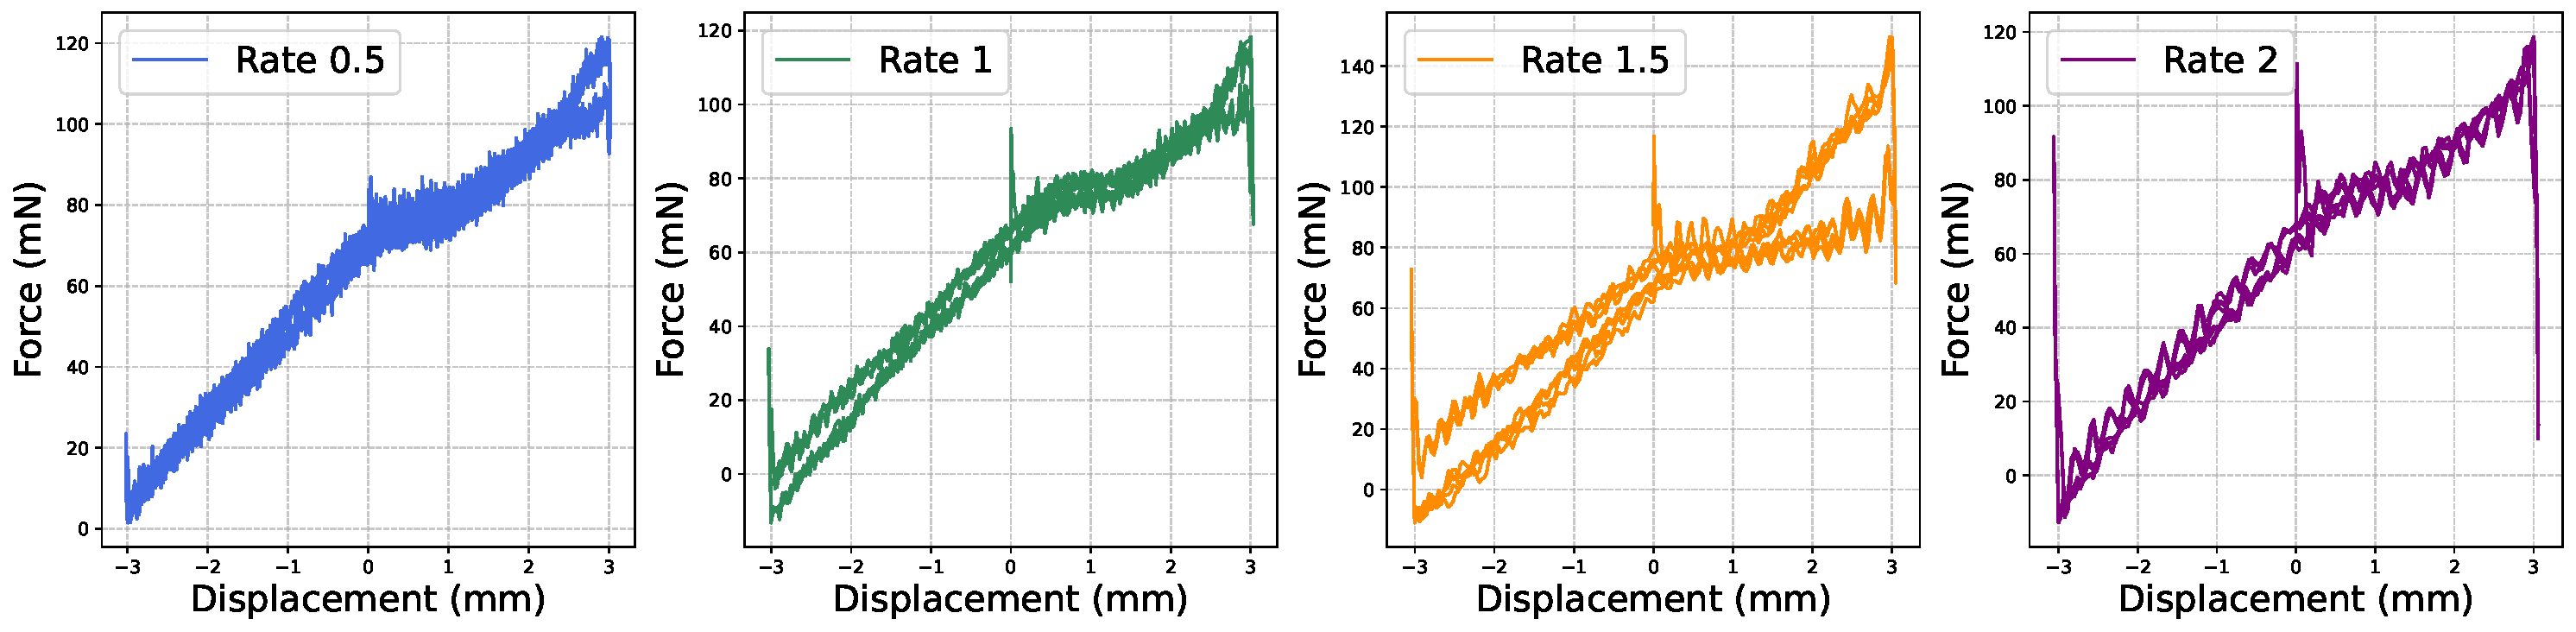
\includegraphics[width=\textwidth]{instron_actuator_calibration.pdf}
    \end{center}
    \caption{\textbf{Force-displacement curves of one actuator at different speeds. }}
    \label{fig:instron_actuator_calibration}
\end{figure}

\section{Multiple scale expansion derivation}
\label{subsec:2units_mse_derivation}


In this section we analyse the classical dynamical equations of two non-reciprocal oscillators (units) coupled together via a viscoelastic band. 
Each unit contains two actuators. The configuration is displayed in figure \ref{fig:diagram_2units}.
We use the method of multiple scales to find the complex amplitude equations describing the slow dynamics of the system. 
Next we switch to polar variables: real amplitude and phase. Finally, we interpret the results in terms of synchronization between the two oscillators.

Since there are 2 actuators per non-reciprocal unit, we have 4 actuators and 8 degrees of freedom in total. 
We denote the displacements of the actuators in unit 1 as $x_{1\alpha}$ and $x_{1\beta}$, and in unit 2 as $x_{2\alpha}$ and $x_{2\beta}$. 
The actuators follow classical mechanics laws, so we can use Newton's second law to write down the equations of motion:

\begin{equation}
\begin{aligned}
\ddot{x}_{1\alpha} + \omega^2 x_{1\alpha} &= 
\epsilon(\omega^2 - \omega_{1\alpha}^2) x_{1\alpha}
-\epsilon \gamma_{1\alpha} \dot{x}_{1\alpha}
- \epsilon k_{c,1\alpha} x_{1\alpha}^3
+ \epsilon k_a^{1} x_{1\beta} 
+ \epsilon k_v (\dot{x}_{2\alpha} - \dot{x}_{1\alpha})
+ \frac{\epsilon k_b}{2 l^2} (x_{2\alpha} - x_{1\alpha})^3, \\
\ddot{x}_{1\beta} + \omega^2 x_{1\beta} &= 
\epsilon(\omega^2 - \omega_{1\beta}^2) x_{1\beta}
-\epsilon \gamma_{1\beta} \dot{x}_{1\beta}
- \epsilon k_{c,1\beta} x_{1\beta}^3
- \epsilon k_a^{1} x_{1\alpha}
+ \epsilon k_v (\dot{x}_{2\beta} - \dot{x}_{1\beta})
+ \frac{\epsilon k_b}{2 l^2} (x_{2\beta} - x_{1\beta})^3, \\
\ddot{x}_{2\alpha} + \omega^2 x_{2\alpha} &= 
\epsilon(\omega^2 - \omega_{2\alpha}^2) x_{2\alpha}
-\epsilon \gamma_{2\alpha} \dot{x}_{2\alpha}
- \epsilon k_{c,2\alpha} x_{2\alpha}^3
+ \epsilon k_a^{2} x_{2\beta} 
+ \epsilon k_v (\dot{x}_{1\alpha} - \dot{x}_{2\alpha})
+ \frac{\epsilon k_b}{2 l^2} (x_{1\alpha} - x_{2\alpha})^3, \\
\ddot{x}_{2\beta} + \omega^2 x_{2\beta} &= 
\epsilon(\omega^2 - \omega_{2\beta}^2) x_{2\beta}
-\epsilon \gamma_{2\beta} \dot{x}_{2\beta}
- \epsilon k_{c,2\beta} x_{2\beta}^3
- \epsilon k_a^{2} x_{2\alpha}
+ \epsilon k_v (\dot{x}_{1\beta} - \dot{x}_{2\beta})
+ \frac{\epsilon k_b}{2 l^2} (x_{1\beta} - x_{2\beta})^3,
\end{aligned}
\end{equation}
where $\omega_{u\sigma}$ is the natural frequency of actuator $\sigma\in\{\alpha,\beta\}$ in unit $u\in\{1,2\}$, 
$\gamma_{u\sigma}$ is the damping coefficient, $k_{c,u\sigma}$ is the nonlinear saturation stiffness,
$k_a^{u}$ is the non-reciprocal coupling within unit $u$, $k_b$ and $k_v$ 
are the elastic and viscous coupling strengths of the viscoelastic band, and $l$ 
is the distance between the actuators at rest. The parameter $\epsilon$ indicates that all the perturbations, 
detuning, damping, nonlinear stiffness, non-reciprocal coupling and neighbour couplings, are weak compared to the harmonic oscillator terms.

The first step is to perform the multiple scale expansion. We skip some of the details as we already presented them before. 
The result is a set of 4 coupled complex amplitude equations describing the slow dynamics of the system. 
The solution at order $\epsilon^0$ is 
\begin{equation}
    x_{u\sigma}^0 = A_{u\sigma}(T)e^{i\omega t} + A_{u\sigma}^*(T)e^{-i\omega t},
\end{equation}
for all actuators ($u=1,2$, $\sigma\in\{\alpha,\beta\}$). When plugging the above formula in the cubic term of the 
$\mathcal{O}(\epsilon)$ equation, one gets
\begin{equation}
    (x_{u\sigma}^0)^3 = A_{u\sigma}^3 e^{3i\omega t} + 3\underbrace{A_{u\sigma}^2 A_{u\sigma}^*}_{|A_{u\sigma}|^2 A_{u\sigma}} e^{i\omega t} 
    + \underbrace{3|A_{u\sigma}|^2 A_{u\sigma}^* e^{-i\omega t} + (A_{u\sigma}^*)^3 e^{-3i\omega t}}_{+\text{ c.c.}}.
\end{equation}
For the neighbour coupling term between the $\alpha$-actuators in the two units, we do a similar procedure, but now we have two different oscillators. 
The full term is 
\begin{equation}
    (x_{2\alpha} - x_{1\alpha})^3 = x_{2\alpha}^3 - 3x_{2\alpha}^2 x_{1\alpha} + 3x_{2\alpha} x_{1\alpha}^2 - x_{1\alpha}^3.
\end{equation}
Before raising to the third power, we can substitute the $\mathcal{O}(\epsilon^0)$ solution for $x_{2\alpha}$ and $x_{1\alpha}$:
\begin{equation}
x_{2\alpha}^0 - x_{1\alpha}^0 = \underbrace{(A_{2\alpha} - A_{1\alpha})}_{B} e^{i \omega t} 
+ \underbrace{(A_{2\alpha}^* - A_{1\alpha}^*)}_{B^*} e^{-i \omega t} = \Delta.
\end{equation}
Raising to the cube, we find terms with frequencies $3\omega$, $-3\omega$, $\omega$ and $-\omega$. 
The terms with frequencies $3\omega$ and $-3\omega$ disappear when applying the solvability condition, since 
they are the only terms with those frequencies, and they must be set to zero.
We can ignore them. The only term that survives is the one with frequency $\omega$, which is given by
\begin{equation}
\Delta^3 = \underbrace{B^3 e^{3i \omega t}}_{\text{vanish}} + 3 |B|^2 B e^{i \omega t} + 3 |B|^2 B^* e^{-i \omega t} 
+ \underbrace{B^{*3} e^{-3i \omega t}}_{\text{vanish}}
 = 3 |A_{2\alpha} - A_{1\alpha}|^2 (A_{2\alpha} - A_{1\alpha}) e^{i \omega t} + \text{c.c.}
\end{equation}

Recall the identities from the multiple scale expansion:
\begin{equation}
x_{u\sigma} = x_{u\sigma}^0 + \epsilon x_{u\sigma}^1 \quad \text{and} \quad \frac{d}{dt} = \partial_t + \epsilon \partial_T.
\end{equation}
Substituting the above identities in the equations of motion, and looking at order $\mathcal{O}(\epsilon^1)$, 
we get the following equation for the first actuator in unit 1:
\begin{multline}
\epsilon^1:\quad 
\partial_{tt} x_{1\alpha}^1 - 2\partial_{tT} x_{1\alpha}^0 + \omega^2 x_{1\alpha}^1 = \\
(\omega^2 - \omega_{1\alpha}^2)x_{1\alpha}^0 - \gamma_{1\alpha} \dot{x}_{1\alpha}^0 
- k_{c,1\alpha}(x_{1\alpha}^0)^3 + k_a^{1} x_{1\beta}^0 + k_v (\dot{x}_{2\alpha}^0 - \dot{x}_{1\alpha}^0) 
+ \frac{k_b}{2l^2}(x_{2\alpha}^0 - x_{1\alpha}^0)^3.
\end{multline}
Let's look at mode $e^{i \omega t}$ and apply the solvability condition:
 \begin{multline}
(\omega^2 - \omega_{1\alpha}^2) A_{1\alpha} - i \omega \gamma_{1\alpha} A_{1\alpha} - 2i \omega A_{1\alpha}' 
- 3k_{c,1\alpha} |A_{1\alpha}|^2 A_{1\alpha} \\ 
+ k_a^{1} A_{1\beta} 
+ i\omega k_v (A_{2\alpha} - A_{1\alpha}) + \frac{k_b}{2l^2} 3 |A_{2\alpha} - A_{1\alpha}|^2 (A_{2\alpha} - A_{1\alpha}) = 0.
\end{multline}
Reorganizing the expression we get the Schrödinger-like equation:
\begin{equation}
\begin{split}
i A_{1\alpha}' = \frac{1}{2\omega} \left[ 
\underbrace{(\omega^2 - \omega_{1\alpha}^2)}_{(\omega - \omega_{1\alpha})(\omega + \omega_{1\alpha})\approx 2\omega(\omega - \omega_{1\alpha})} A_{1\alpha} 
- i \omega \gamma_{1\alpha} A_{1\alpha} - 3k_{c,1\alpha} |A_{1\alpha}|^2 A_{1\alpha} 
+ k_a^{1} A_{1\beta} \right. \\
\left. \vphantom{\underbrace{(\omega^2 - \omega_{1\alpha}^2)}_{(\omega - \omega_{1\alpha})(\omega + \omega_{1\alpha})\approx 2\omega(\omega - \omega_{1\alpha})}}
+ \frac{ik_v}{2} (A_{2\alpha} - A_{1\alpha}) + \frac{3k_b}{2l^2} |A_{2\alpha} - A_{1\alpha}|^2 (A_{2\alpha} - A_{1\alpha}) \right].
\end{split}
\end{equation}

After simplifying the expression, we get the complex amplitude equation for the first actuator in unit 1:
\begin{align}
A_{1\alpha}' =& -i(\omega - \omega_{1\alpha}) A_{1\alpha} - \frac{1}{2} \gamma_{1\alpha} A_{1\alpha} 
+ \frac{3i k_{c,1\alpha}}{2\omega} |A_{1\alpha}|^2 A_{1\alpha} \\
&+ \frac{3i k_a^{1}}{2\omega} A_{1\beta} 
+ \frac{k_v}{2} (A_{2\alpha} - A_{1\alpha}) - \frac{3i k_b}{4\omega l^2} |A_{2\alpha} - A_{1\alpha}|^2 (A_{2\alpha} - A_{1\alpha})
\label{eq_MSE_2nodes_complex_amplitude}
\end{align}

The next step is to rewrite everything in terms of the polar variables $A_{u\sigma} = R_{u\sigma}(T) e^{i\phi_{u\sigma}(T)}$ and simplify: 

\begin{equation}
|A_{1\alpha}|^2 = R_{1\alpha}^2 \qquad |A_{2\alpha} - A_{1\alpha}|^2 = \left| R_{2\alpha} e^{i\phi_{2\alpha}} - R_{1\alpha} e^{i\phi_{1\alpha}} \right|^2
\end{equation}

The second term can be worked out:
\begin{equation}
 \left(R_{2\alpha} e^{i\phi_{2\alpha}} - R_{1\alpha} e^{i\phi_{1\alpha}}\right) 
 \left(R_{2\alpha} e^{-i\phi_{2\alpha}} - R_{1\alpha} e^{-i\phi_{1\alpha}}\right) \\
= R_{2\alpha}^2 + R_{1\alpha}^2 - 2R_{2\alpha} R_{1\alpha} \cos(\phi_{2\alpha} - \phi_{1\alpha})
\end{equation}

Multiplying the previous expression by $(A_{2\alpha} - A_{1\alpha})$:

\begin{equation}
\begin{aligned}
&\cdot (A_{2\alpha} - A_{1\alpha}) \rightarrow 
\left( R_{2\alpha}^2 + R_{1\alpha}^2 - 2R_{2\alpha} R_{1\alpha} \cos(\phi_{2\alpha} - \phi_{1\alpha}) \right) 
\left(R_{2\alpha} e^{i\phi_{2\alpha}} - R_{1\alpha} e^{i\phi_{1\alpha}}\right) = \\
&= R_{2\alpha}^3 e^{i\phi_{2\alpha}} + R_{1\alpha}^2 R_{2\alpha} e^{i\phi_{2\alpha}} 
- 2R_{2\alpha}^2 R_{1\alpha} \cos(\phi_{2\alpha} - \phi_{1\alpha}) e^{i\phi_{2\alpha}} \\
&\quad - R_{2\alpha}^2 R_{1\alpha} e^{i\phi_{1\alpha}} - R_{1\alpha}^3 e^{i\phi_{1\alpha}} 
+ 2R_{2\alpha} R_{1\alpha}^2 \cos(\phi_{2\alpha} - \phi_{1\alpha}) e^{i\phi_{1\alpha}}
\label{eq_MSE_2nodes_cubic}
\end{aligned}
\end{equation}

We separate the real part, which will be the one associated to the radius/amplitude: 

\begin{equation}
\begin{aligned}
\text{Re}\left[ |A_{2\alpha} - A_{1\alpha}|^2 (A_{2\alpha} - A_{1\alpha}) \right] &= 
R_{2\alpha}^3 \cos\phi_{2\alpha} + R_{1\alpha}^2 R_{2\alpha} \cos\phi_{2\alpha} \\
&\quad - 2R_{2\alpha}^2 R_{1\alpha} \cos(\phi_{2\alpha} - \phi_{1\alpha}) \cos\phi_{2\alpha} \\
&\quad - R_{2\alpha}^2 R_{1\alpha} \cos\phi_{1\alpha} - R_{1\alpha}^3 \cos\phi_{1\alpha} \\
&\quad + 2R_{2\alpha} R_{1\alpha}^2 \cos(\phi_{2\alpha} - \phi_{1\alpha}) \cos\phi_{1\alpha}
\end{aligned}
\end{equation}

The imaginary part is very similar with $\sin\phi_{1\alpha}$ or $\sin\phi_{2\alpha}$ terms instead of cosines.

Putting everything back into equation \eqref{eq_MSE_2nodes_amplitude} after substituting the polar variables, we find:

\begin{equation}
\begin{aligned}
\dot{R}_{1\alpha} e^{i\phi_{1\alpha}} + i R_{1\alpha} \dot{\phi}_{1\alpha} e^{i\phi_{1\alpha}} &= 
-i(\omega - \omega_{1\alpha}) R_{1\alpha} e^{i\phi_{1\alpha}} - \frac{1}{2} \gamma_{1\alpha} R_{1\alpha} e^{i\phi_{1\alpha}} 
 + \frac{3ik_{c,1\alpha}}{2\omega} R_{1\alpha}^3 e^{i\phi_{1\alpha}} - \frac{3ik_a^{1}}{2\omega} R_{1\beta} e^{i\phi_{1\beta}} \\
&\quad + \frac{k_v}{2} (R_{2\alpha}e^{i\phi_{2\alpha}} - R_{1\alpha}e^{i\phi_{1\alpha}}) 
- \frac{3ik_b}{4\omega l^2} [\text{ equation \eqref{eq_MSE_2nodes_cubic}}]
\end{aligned}
\end{equation}
We can multiply both sides by $e^{-i\phi_{1\alpha}}$. 
\begin{equation}
\begin{aligned}
\dot{R}_{1\alpha} + i R_{1\alpha} \dot{\phi}_{1\alpha} &= 
-i(\omega - \omega_{1\alpha}) R_{1\alpha} - \frac{1}{2} \gamma_{1\alpha} R_{1\alpha} 
+ \frac{3ik_{c,1\alpha}}{2\omega} R_{1\alpha}^3 - \frac{3ik_a^{1}}{2\omega} R_{1\beta} e^{i(\phi_{1\beta} - \phi_{1\alpha})} \\
&\quad + \frac{k_v}{2} (R_{2\alpha}e^{i(\phi_{2\alpha}-\phi_{1\alpha})} - R_{1\alpha}) 
- \frac{3ik_b}{4\omega l^2} \left[ e^{i(\phi_{2\alpha} - \phi_{1\alpha})} 
\left( R_{2\alpha}^3 + R_{1\alpha}^2 R_{2\alpha} - 2R_{2\alpha}^2 R_{1\alpha} \cos(\phi_{2\alpha} - \phi_{1\alpha}) \right) \right. \\
&\quad \left. - R_{2\alpha}^2 R_{1\alpha} - R_{1\alpha}^3 + 2R_{2\alpha} R_{1\alpha}^2 \cos(\phi_{2\alpha} - \phi_{1\alpha}) \right]
\end{aligned}
\end{equation}
We observe that the real part is associated to 
the radius/amplitude dynamics, while the imaginary part is associated to the phase dynamics.
We take the real and imaginary parts of the previous expression. The real part is:

\begin{equation}
\begin{aligned}
\dot{R}_{1\alpha} &= -\frac{1}{2} \gamma_{1\alpha} R_{1\alpha} 
+ \frac{3k_a^{1}}{2\omega} R_{1\beta} \sin(\phi_{1\beta} - \phi_{1\alpha}) 
+ \frac{k_v}{2} (R_{2\alpha}\cos{(\phi_{2\alpha} - \phi_{1\alpha})} - R_{1\alpha}) \\
&\quad + \frac{3k_b}{4\omega l^2} \sin(\phi_{2\alpha} - \phi_{1\alpha}) 
\left( R_{2\alpha}^3 + R_{1\alpha}^2 R_{2\alpha} - 2R_{2\alpha}^2 R_{1\alpha} \cos(\phi_{2\alpha} - \phi_{1\alpha}) \right)
\end{aligned}
\end{equation}

The imaginary part of the equation is:

\begin{equation}
\begin{aligned}
R_{1\alpha} \dot{\phi}_{1\alpha} &= 
-(\omega - \omega_{1\alpha}) R_{1\alpha} + \frac{3k_{c,1\alpha}}{2\omega} R_{1\alpha}^3 
- \frac{3k_a^{1}}{2\omega} R_{1\beta} \cos(\phi_{1\beta} - \phi_{1\alpha}) 
+ \frac{k_v}{2} (R_{2\alpha}\sin{(\phi_{2\alpha} - \phi_{1\alpha})} - R_{1\alpha}) \\
&\quad - \frac{3k_b}{4\omega l^2} \left[ \cos(\phi_{2\alpha} - \phi_{1\alpha}) 
\left( R_{2\alpha}^3 + R_{1\alpha}^2 R_{2\alpha} - 2R_{2\alpha}^2 R_{1\alpha} \cos(\phi_{2\alpha} - \phi_{1\alpha}) \right) \right. \\
&\quad \left. - R_{2\alpha}^2 R_{1\alpha} - R_{1\alpha}^3 
+ 2R_{2\alpha} R_{1\alpha}^2 \cos(\phi_{2\alpha} - \phi_{1\alpha}) \right]
\end{aligned}
\end{equation}

Dividing the imaginary part by $R_{1\alpha}$ yields the phase dynamics for $\dot{\phi}_{1\alpha}$:

\begin{equation}
\begin{aligned}
\dot{\phi}_{1\alpha} &= 
-(\omega - \omega_{1\alpha}) + \frac{3k_{c,1\alpha}}{2\omega} R_{1\alpha}^2 
- \frac{3k_a^{1}}{2\omega} \frac{R_{1\beta}}{R_{1\alpha}} \cos(\phi_{1\beta} - \phi_{1\alpha}) 
+ \frac{k_v}{2} \left(\frac{R_{2\alpha}}{R_{1\alpha}}\sin{(\phi_{2\alpha} - \phi_{1\alpha})} - 1\right) \\
&\quad - \frac{3k_b}{4\omega l^2} \left[ \cos(\phi_{2\alpha} - \phi_{1\alpha}) 
\left( \frac{R_{2\alpha}^3}{R_{1\alpha}} + R_{1\alpha} R_{2\alpha} - 2R_{2\alpha}^2 \cos(\phi_{2\alpha} - \phi_{1\alpha}) \right) \right. \\
&\quad \left. - R_{2\alpha}^2 - R_{1\alpha}^2 + 2R_{2\alpha} R_{1\alpha} \cos(\phi_{2\alpha} - \phi_{1\alpha}) \right]
\end{aligned}
\end{equation}

The equations for the other actuators ($1\beta$, $2\alpha$, $2\beta$) are obtained in the same way and they will just differ in some of the indices. 
We have arrived at the envelope/Stuart-Landau equations of two non-reciprocal units coupled via a viscoelastic band. We can 
compare the coefficients of \eqref{eq_MSE_2nodes_phase} with experimental data. Note that equation \eqref{eq_MSE_2nodes_phase} 
resembles a Kuramoto-type of model. The first term is the natural frequency of the spring. 
The second term is a non-isochronous term. It means that how large the radius is affects the frequency of oscillation. 
The third term is a usual Kuramoto coupling between two oscillators. The important feature here is that 
the coupling is proportional to the ratio of radii $\frac{R_{2\alpha}}{R_{1\alpha}}$. The last term is a more complicated Kuramoto-type 
of coupling, which is a consequence of the cubic neighbour coupling.

We can also consider some simplified limits of equations \eqref{eq_MSE_2nodes_amplitude} and \eqref{eq_MSE_2nodes_phase}. 
Actuators $\alpha$ and $\beta$ in each unit are coupled non-reciprocally, so their phase difference is 
$|\phi_{1\beta} - \phi_{1\alpha}| = \pi/2$ and $|\phi_{2\beta} - \phi_{2\alpha}| = \pi/2$. 
This means that the non-reciprocal coupling term is maximal in the radius equation, and it is zero in the phase equation.
We can also consider the synchronization regime, when the limit cycles of units 1 and 2 oscillate with same frequency. 
In the case of complete synchronization between the $\alpha$-actuators, both have the same phase: $\phi_{2\alpha} = \phi_{1\alpha}$. 
In this limit, the neighbour coupling term in the amplitude equation vanishes, and the neighbour coupling term simplifies. 

\begin{align}
\dot{R}_{1\alpha} &= -\frac{1}{2} \gamma_{1\alpha} R_{1\alpha} + \frac{3k_a^{1}}{2\omega} R_{1\beta} 
+ \frac{k_v}{2} (R_{2\alpha} - R_{1\alpha}) \\ %\label{eq_sync_amplitude_simplified}\\
\dot{\phi}_{1\alpha} &= -(\omega - \omega_{1\alpha}) + \frac{3k_{c,1\alpha}}{2\omega} R_{1\alpha}^2  
- \frac{k_v}{2} + \frac{3k_b}{4\omega l^2} \frac{(R_{2\alpha}-R_{1\alpha})^2}{R_{1\alpha}}
\end{align}

We can take the phase dynamics approximation, and to be valid it requires the RHS of equation \eqref{eq_sync_amplitude_simplified} to be zero.
That gives a constraint on the radii of the actuators and the damping coefficient: 
$R_{1\beta} = \frac{\omega \gamma_{1\alpha}}{3k_a^{1}} R_{1\alpha}$.
By considering also the $\dot{R}_{1\beta}$ equation and the same simplifying assumptions, we obtain a
relation between the radii of the actuators inside the unit and the damping coefficient:

\begin{equation}
    \frac{\gamma_{1\alpha}}{\gamma_{1\beta}} = \left(\frac{R_{1\beta}}{R_{1\alpha}}\right)^2
\end{equation}

The equation seems reasonable. The higher the damping for one of the springs inside a non-reciprocal unit, 
the smaller its amplitude of oscillation. 

If the neighbour coupling was linear instead of cubic, we would have obtained 
\begin{equation}
    k_b (A_{2\alpha} - A_{1\alpha}) = k_b (R_{2\alpha} e^{i\phi_{2\alpha}} - R_{1\alpha} e^{i\phi_{1\alpha}}) 
    \longrightarrow k_b \left( 1- \frac{R_{2\alpha}}{R_{1\alpha}} \cos(\phi_{2\alpha} - \phi_{1\alpha}) \right).
\end{equation}
If we view this term as a Kuramoto-type of coupling, we see that the coupling constant is given by $k_b R_{2\alpha}/R_{1\alpha}$. 
When doing experiments at first, the individual amplitude of oscillations of 2 \textit{uncoupled} non-reciprocal 
units was different. And when they were coupled with the viscoelastic band, the amplitudes changed in a nontrivial way. 
I suspected that the amplitude had an effect on the Kuramoto coupling. My guess was that if we have the Kuramoto system 
\begin{equation}
    \dot{\Theta}_1 = \omega_1 + K_1 \sin(\Theta_2 - \Theta_1) \\
    \dot{\Theta}_2 = \omega_2 + K_2 \sin(\Theta_1 - \Theta_2), 
\end{equation}
then the coupling constants were proportional to the other oscillator's amplitude: $K_1 \propto R_{2\alpha}$ and $K_2 \propto R_{1\alpha}$.
This ansatz explained the qualitative behaviour of the synchronization frequency and amplitude of the coupled system. 
However, it didn't explain the quantitative results. One reason that could explain this disagreement is 
the fact that the coupling is not linear, but cubic. 
The neighbour coupling term is given by $|A_{2\alpha} - A_{1\alpha}|^2 (A_{2\alpha} - A_{1\alpha})$, which is a more complicated function 
of the amplitudes and phases of the oscillators.

%%%%%%%%%%%%%%%%%%%%%%%%%%%%%%%%%%%%%%%%%%%%%%%% phase difference between 2 units (phi_{2\alpha} and phi_{1\alpha})
Assuming that both units are tracing out stable limit cycles, so the phase differences are 
$\phi_{1\beta} - \phi_{1\alpha} = \pi/2 = \phi_{2\beta} - \phi_{2\alpha}$
and the radii are fixed $\dot{R}_{u\sigma}=0$, the whole dynamical system reduces to 
\begin{align}
    \dot{\phi}_{1\alpha} &=  \omega_{1\alpha} + \frac{3k_{c,1\alpha}}{2\omega} R_{1\alpha}^2 
    + \frac{k_v}{2} \left(\frac{R_{2\alpha}}{R_{1\alpha}}\sin{(\phi_{2\alpha} - \phi_{1\alpha})} - 1\right) 
    + [k_b \;\text{terms}]\\
 \dot{\phi}_{2\alpha} &=  \omega_{2\alpha} + \frac{3k_{c,2\alpha}}{2\omega} R_{2\alpha}^2 
 + \frac{k_v}{2} \left(\frac{R_{1\alpha}}{R_{2\alpha}}\sin{(\phi_{1\alpha} - \phi_{2\alpha})} - 1\right) 
     + [k_b \;\text{terms}].
\end{align}
We are interested in the phase difference between the two units $\Delta\phi = \phi_{2\alpha} - \phi_{1\alpha}$. 

The dynamics of the phase difference is:
\begin{equation}
    \dot{\Delta\phi} = \omega_{2\alpha} - \omega_{1\alpha} 
    + \frac{3}{2\omega}\left(k_{c,2\alpha}R_{2\alpha}^2 - k_{c,1\alpha}R_{1\alpha}^2\right) 
    - \frac{k_v}{2}\sin{\Delta\phi} \left(\frac{R_{2\alpha}}{R_{1\alpha}} + \frac{R_{1\alpha}}{R_{2\alpha}}\right) 
    + [k_b \;\text{terms}]
\end{equation}
To simplify further, we consider identical oscillators $R_{1\alpha}=R_{2\alpha},\quad k_{c,1\alpha}=k_{c,2\alpha}$. 
Note that the $k_b$ terms are even due to the cosine function. Since we subtract two identical even functions 
(with opposite argument $-\Delta\phi$), they cancel out. 
The expression nicely simplifies to 
\begin{equation}
    \dot{\Delta\phi} = \underbrace{\omega_{2\alpha} - \omega_{1\alpha}}_{\text{detuning}} - k_v\sin{\Delta\phi},
\end{equation}
which is precisely the Adler equation. The assumptions made were: identical units, quadrature phase within each unit, 
and stable limit cycles of individual units.

\section{Two units}
\label{subsec:annex_2units_same_chirality}
In figure \ref{2_nodes_same_chir_repeated_phase}, we show the experimental data of the phase difference between two units with the same 
chirality. We can clearly see constant lines that correspond to phase locking. There are also
occasional phase slips. The figure justifies studying the frequency changes from uncoupled to coupled units.
\begin{figure}[hbtp]
    \begin{center}
        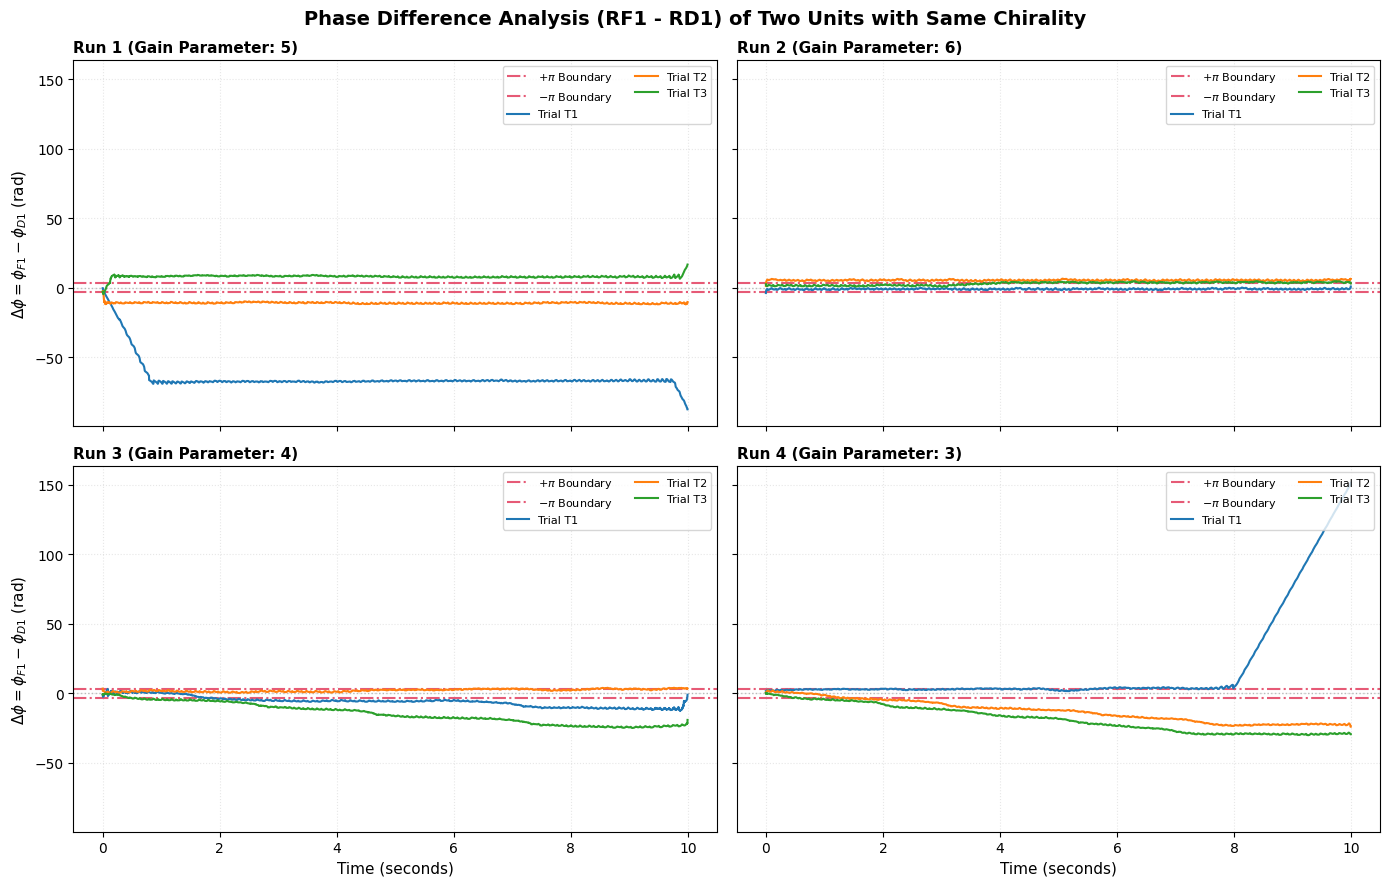
\includegraphics[width = 0.8\textwidth]{2_nodes_same_chir_repeated_phase.png}
        \caption{Phase Difference Analysis of Two Units with Same Chirality}
        \label{2_nodes_same_chir_repeated_phase}
    \end{center}
\end{figure}

\section{1D chain}

\begin{figure}[htbp]
  \centering
  \begin{subfigure}[b]{\textwidth}
    \centering
    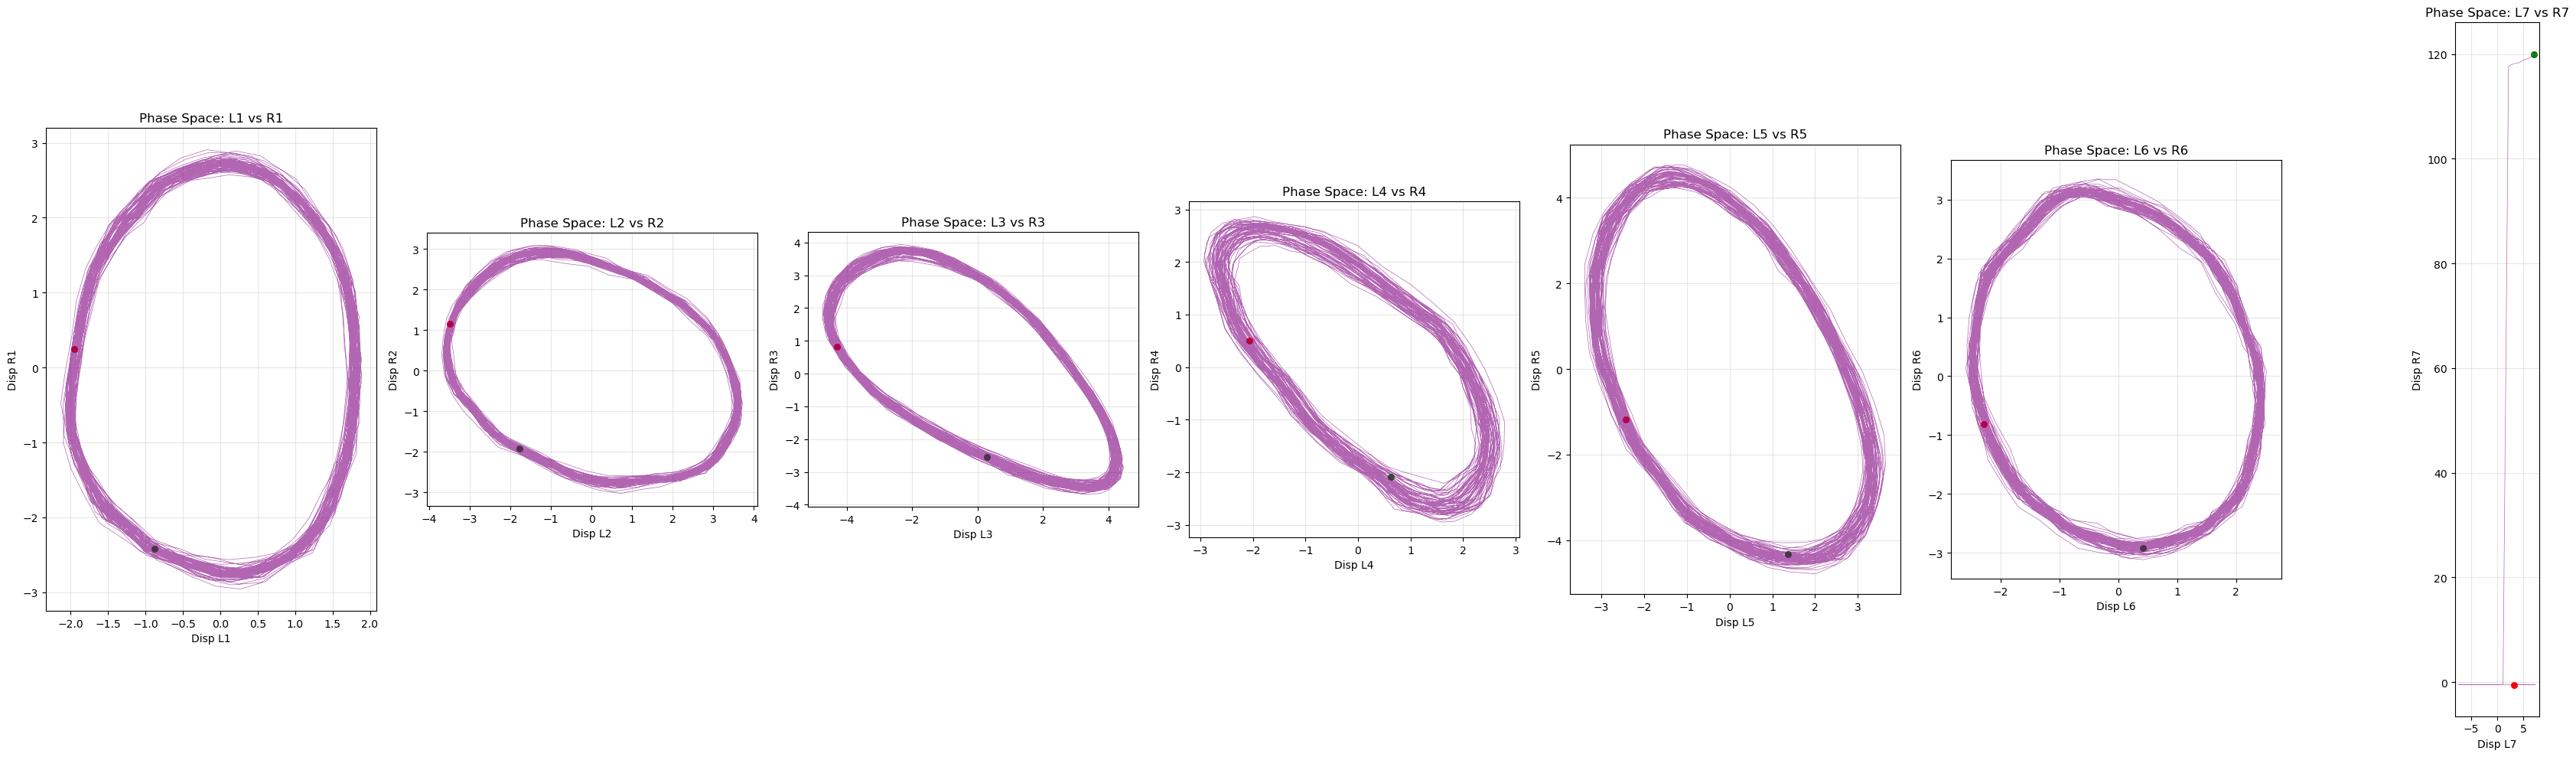
\includegraphics[width=\textwidth]{limit_cycles_same_chir.png}
    \caption{Limit cycles of nodes with same chirality in 1d strip. 
    Results are from measurements done 17-3-2026 Try 1.}
    \label{fig:top-plot}
  \end{subfigure}

  \vspace{1em}

  \begin{subfigure}[b]{\textwidth}
    \centering
    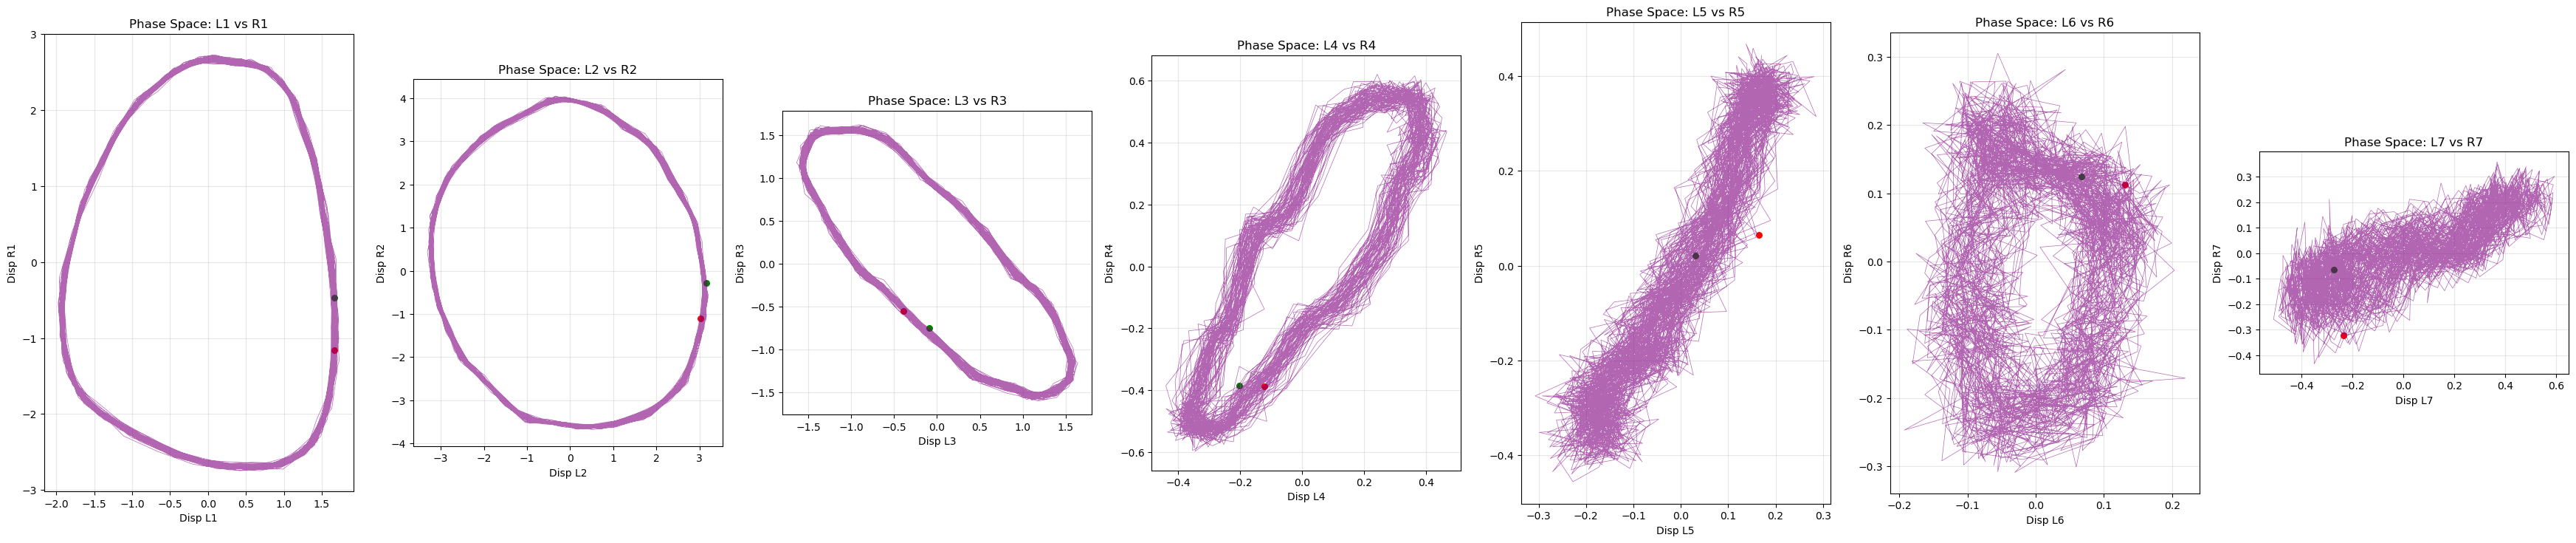
\includegraphics[width=\textwidth]{limit_cycles_opp_chir.png}
    \caption{Limit cycles of nodes with opposite chirality in 1d strip.
    Results are from measurements done 13-3-2026 Try 1.}
    \label{fig:bottom-plot}
  \end{subfigure}

  \caption{Comparison of limit cycles for same and opposite chirality scenarios in the 1D strip.}
  \label{fig:stacked-plots}
\end{figure}

\begin{figure}[htbp]
  \centering
  \begin{subfigure}[b]{0.48\textwidth}
    \centering
    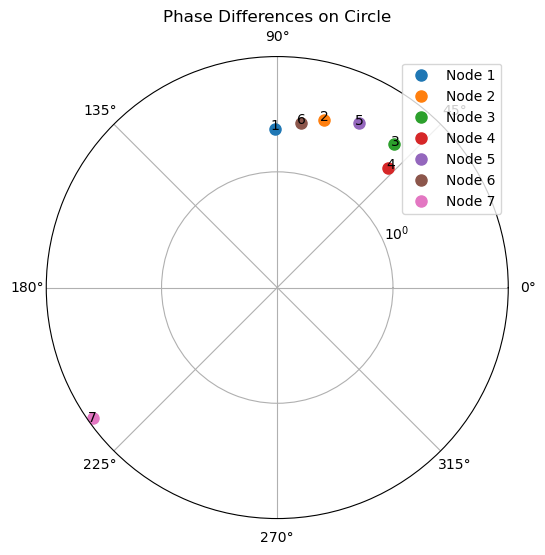
\includegraphics[width=\linewidth]{phase_diff_same_chir.png}
    \caption{Polar plot of phase difference for actuators within the same unit in scenario 
    with same chirality. The results are from 17-3-2026 Try 1.}
    \label{fig:left-plot}
  \end{subfigure}
  \hfill
  \begin{subfigure}[b]{0.48\textwidth}
    \centering
    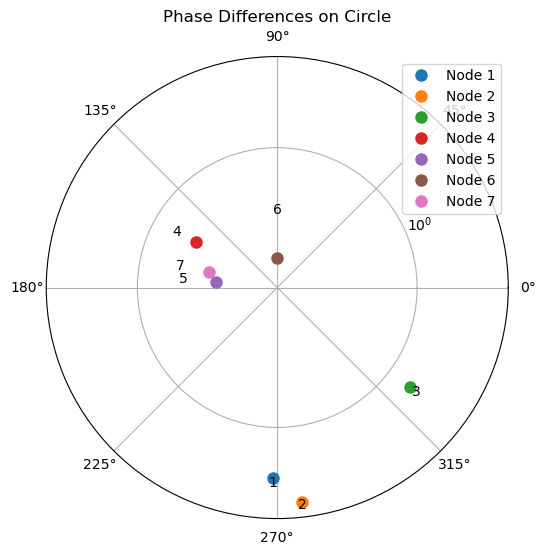
\includegraphics[width=\linewidth]{phase_diff_opp_chir.png}
    \caption{Polar plot of phase difference for actuators within the same unit in scenario 
    with opposite chirality. The results are from 13-3-2026 Try 1.}
    \label{fig:right-plot}
  \end{subfigure}
  \caption{Comparison phase difference of limit cycles for same and 
  opposite chirality scenarios in the 1D strip. The angle in the polar plot 
  corresponds to the phase difference between the two actuators in aunit, 
  and the radius corresponds to the amplitude of the oscillations. More 
  precisely, the radius is the average of the amplitudes of the two actuators in a unit.
  The radius axis is in logarithmic scale to better visualize small amplitudes.}
  \label{fig:side-by-side-plots}
\end{figure}

We can also compare how the limit cycles look in both scenarios: with same and 
with opposite chirality (see figure \ref{fig:stacked-plots}). The results from the same 
chirality (figure \ref{fig:top-plot}) show circular thin limit cycles. The fact that they are circular means 
that the phase difference between the two actuators is 90º. The fact that they are thin 
is a consequence of the oscillations being very stable. In comparison, the limit cycles 
from the opposite chirality scenario (figure \ref{fig:bottom-plot}) are  
not as circular and they are noisier. The fact that they are not circular 
means that the phase difference between the two actuators is not 90º. And they are noisier 
because their oscillation is weaker, and therefore more affected by neighbours. 
And the amplitudes are smaller because the nodes don't synchronize.  

%[I can show plots of FT: what is the punch line?]
As the actuators within a unit can deviate from the non-reciprocal behaviour of 90º, 
we can measure what the phase difference is precisely for each unit. 
Figures \ref{fig:side-by-side-plots} are polar plots of the phase difference. 
For active units with clockwise/negative chirality the phase difference is -90º.
For active units with counterclockwise/positive chirality the phase difference is +90º.
In the scenario where all active units have the same chirality, 
we expect to find those nodes, nodes 2, 4 and 6, in the 90º axis. And that is what 
we observe in figure \ref{fig:left-plot} for nodes 2 and 6. The fact that node 4 
is not close to the 90º axis we think is a consequence of the actuators being crooked. 
In the scenario of opposite chirality, figure \ref{fig:right-plot}, node 2 
has clockwise chirality and nodes 4 and 6 remain with counterclockwise chirality. 
Thus, we expect to find node 2 in the -90º axis and nodes 4 and 6 in the +90º axis. 
Note that in this experiment, node 2 had a higher gain than nodes 4 and 6, and we saw 
that the oscillations of 4 and 6 were suppressed in figure \ref{fig:bottom-plot}. 
That is why these nodes are closer to the origin in the polar plot of figure \ref{fig:right-plot}.
Nevertheless, we still see that node 6 has a strcit phase difference of 90º. 
The phase difference of active units is as one would expect, except for node 4, and 
doesn't add new information. But what happens to the passive units and their phase difference? 


For very disordered activity and a high value of neighbour coupling, one observes a kink in the transient 
process before synchronization. It is shown in figure \ref{fig:kink}. 
The kink corresponds to a unit whose amplitude is very small. It 
propagates back and forth through the chain, changing direction when reaching the ends of the chain. 

\begin{figure}
    \begin{center}
        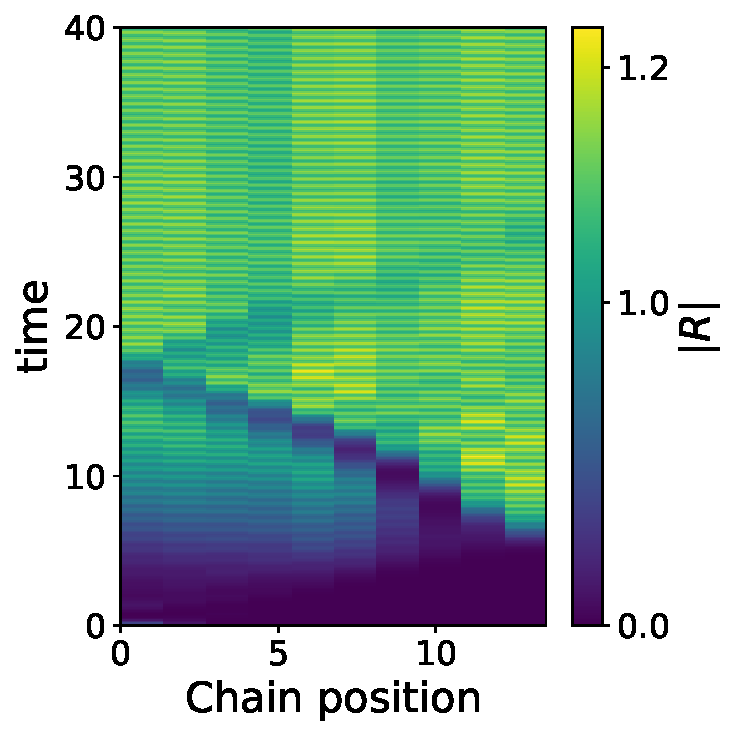
\includegraphics[width=0.5\textwidth]{kink_chain.pdf}
    \end{center}
    \caption{\textbf{Kink in amplitude of 1D chain.}}
    \label{fig:kink}
\end{figure}

\section{Dynamical matrix Lieb lattice}

\begin{figure}[hbtp]
    \centering
        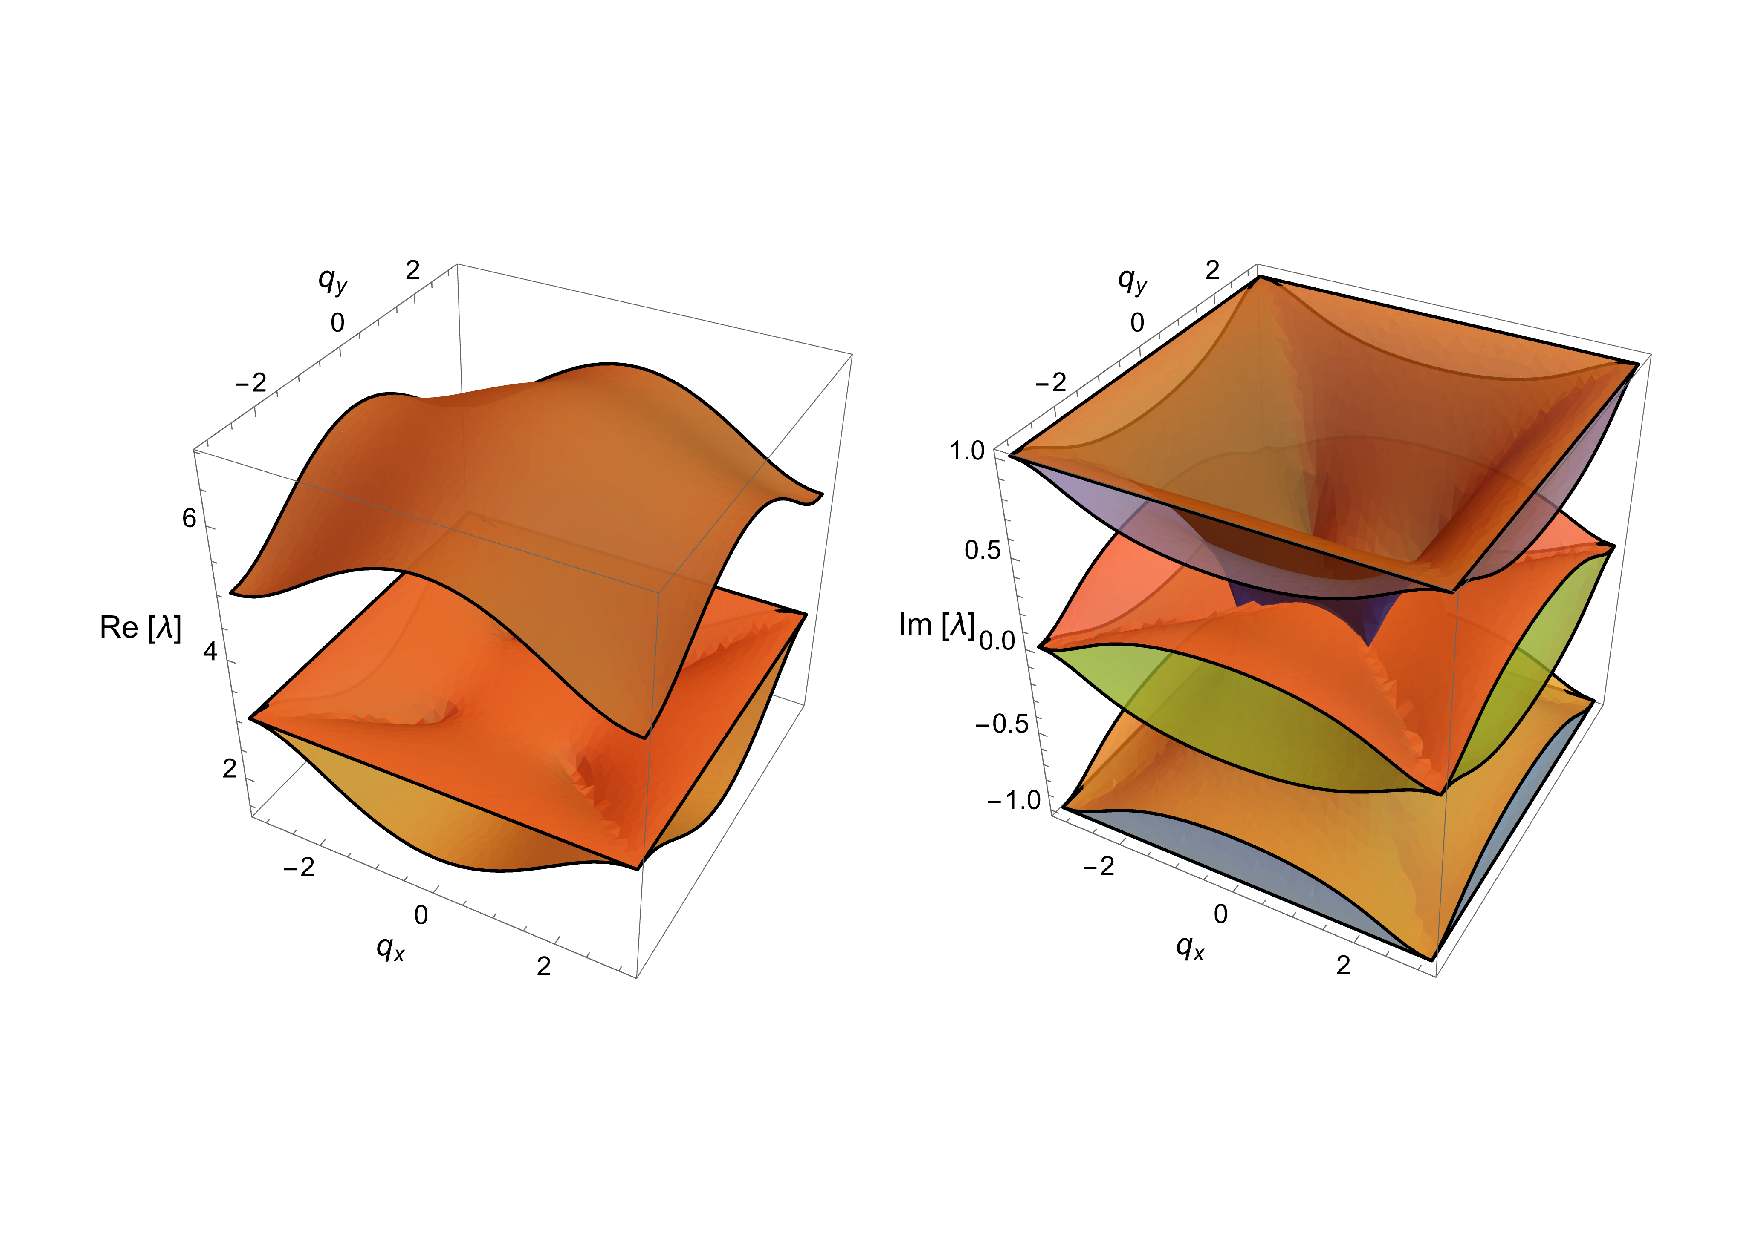
\includegraphics[width=0.85\textwidth, height=0.45\textheight, keepaspectratio]{dispersion_altermagnetic.pdf}
    \caption{Band structure of bilayer Lieb lattice with non-reciprocal couplings. 
    The eigenvalues are computed from the dynamical matrix in equation \eqref{eq:dynamical_matrix}. }
    \label{fig:bands:Lieb_lattice}
\end{figure}

We present the dynamical matrix of a classical Lieb lattice of oscillators with non-reciprocal couplings. 
The matrix is obtained from Newton's equations of motion, and it describes the linearized dynamics of the system. 
We are still considering the bilayer Lieb lattice, so there are 6 sites per unit cell and thus the dynamical matrix 
is a $6\times 6$ matrix. It takes the form in momentum space
\begin{equation}
    \mathbf{D} = \scalebox{0.6}{$
    \begin{pmatrix}
        4k_b + k_0 & k_a \sigma_A & -k_b(1 + e^{-i q_x a}) & 0 & -k_b(1 + e^{-i q_y a}) & 0 \\
        -k_a \sigma_A & 4k_b + k_0 & 0 & -k_b(1 + e^{-i q_x a}) & 0 & -k_b(1 + e^{-i q_y a}) \\
        -k_b(1 + e^{i q_x a}) & 0 & 2k_b + k_0 & k_a \sigma_B & 0 & 0 \\
        0 & -k_b(1 + e^{i q_x a}) & -k_a \sigma_B & 2k_b + k_0 & 0 & 0 \\
        -k_b(1 + e^{i q_y a}) & 0 & 0 & 0 & 2k_b + k_0 & k_a \sigma_C \\
        0 & -k_b(1 + e^{i q_y a}) & 0 & 0 & -k_a \sigma_C & 2k_b + k_0
    \end{pmatrix}.$}
    \label{eq:dynamical_matrix}
\end{equation}
$k_0$ denotes the linear bound strength, $k_b$ the coupling strength between nearest neighbours, 
$k_a$ the non-reciprocal coupling strength, $q_x$ and $q_y$ the momenta in the $x$ and $y$ directions, 
and $\sigma_A$, $\sigma_B$, $\sigma_C$ are the chiralities of the sites A, B and C respectively.
We will choose the chiralities as $\sigma_A = 0$, $\sigma_B = -1$ and $\sigma_C = 1$, 
to reproduce the Lieb lattice. The band structure of the matrix is displayed in
figure \ref{fig:bands:Lieb_lattice}.


\end{appendices}
\end{document}